\documentclass{book}

\usepackage[utf8]{inputenc}
\usepackage[T1]{fontenc}
\usepackage{textcomp}

\usepackage{url}

% \usepackage{hyperref}
% \hypersetup{
%     colorlinks,
%     linkcolor={black},
%     citecolor={black},
%     urlcolor={blue!80!black}
% }

\usepackage{graphicx}
\usepackage{float}
\usepackage[usenames,dvipsnames]{xcolor}

% \usepackage{cmbright}

\usepackage{amsmath, amsfonts, mathtools, amsthm, amssymb}
\usepackage{mathrsfs}
\usepackage{cancel}

% horizontal rule
\newcommand\hr{
    \noindent\rule[0.5ex]{\linewidth}{0.5pt}
}

\usepackage{tikz}
\usepackage{tikz-cd}

% theorems
\usepackage{thmtools}
\usepackage[framemethod=TikZ]{mdframed}
\mdfsetup{skipabove=1em,skipbelow=0em, innertopmargin=5pt, innerbottommargin=6pt}

\theoremstyle{definition}

\makeatletter

\declaretheoremstyle[headfont=\bfseries\sffamily, bodyfont=\normalfont, mdframed={ nobreak } ]{thmgreenbox}
\declaretheoremstyle[headfont=\bfseries\sffamily, bodyfont=\normalfont, mdframed={ nobreak } ]{thmredbox}
\declaretheoremstyle[headfont=\bfseries\sffamily, bodyfont=\normalfont]{thmbluebox}
\declaretheoremstyle[headfont=\bfseries\sffamily, bodyfont=\normalfont]{thmblueline}
\declaretheoremstyle[headfont=\bfseries\sffamily, bodyfont=\normalfont, numbered=no, mdframed={ rightline=false, topline=false, bottomline=false, }, qed=\qedsymbol ]{thmproofbox}
\declaretheoremstyle[headfont=\bfseries\sffamily, bodyfont=\normalfont, numbered=no, mdframed={ nobreak, rightline=false, topline=false, bottomline=false } ]{thmexplanationbox}


\declaretheorem[numberwithin=chapter, style=thmgreenbox, name=Definition]{definition}
\declaretheorem[sibling=definition, style=thmredbox, name=Corollary]{corollary}
\declaretheorem[sibling=definition, style=thmredbox, name=Proposition]{prop}
\declaretheorem[sibling=definition, style=thmredbox, name=Theorem]{theorem}
\declaretheorem[sibling=definition, style=thmredbox, name=Lemma]{lemma}



\declaretheorem[numbered=no, style=thmexplanationbox, name=Proof]{explanation}
\declaretheorem[numbered=no, style=thmproofbox, name=Proof]{replacementproof}
\declaretheorem[style=thmbluebox,  numbered=no, name=Exercise]{ex}
\declaretheorem[style=thmbluebox,  numbered=no, name=Example]{eg}
\declaretheorem[style=thmblueline, numbered=no, name=Remark]{remark}
\declaretheorem[style=thmblueline, numbered=no, name=Note]{note}

\renewenvironment{proof}[1][\proofname]{\begin{replacementproof}}{\end{replacementproof}}

\AtEndEnvironment{eg}{\null\hfill$\diamond$}%

\newtheorem*{uovt}{UOVT}
\newtheorem*{notation}{Notation}
\newtheorem*{previouslyseen}{As previously seen}
\newtheorem*{problem}{Problem}
\newtheorem*{observe}{Observe}
\newtheorem*{property}{Property}
\newtheorem*{intuition}{Intuition}


\usepackage{etoolbox}
\AtEndEnvironment{vb}{\null\hfill$\diamond$}%
\AtEndEnvironment{intermezzo}{\null\hfill$\diamond$}%




% http://tex.stackexchange.com/questions/22119/how-can-i-change-the-spacing-before-theorems-with-amsthm
% \def\thm@space@setup{%
%   \thm@preskip=\parskip \thm@postskip=0pt
% }

\usepackage{xifthen}

\def\testdateparts#1{\dateparts#1\relax}
\def\dateparts#1 #2 #3 #4 #5\relax{
    \marginpar{\small\textsf{\mbox{#1 #2 #3 #5}}}
}

\def\@lesson{}%
\newcommand{\lesson}[3]{
    \ifthenelse{\isempty{#3}}{%
        \def\@lesson{Lecture #1}%
    }{%
        \def\@lesson{Lecture #1: #3}%
    }%
    \subsection*{\@lesson}
    \testdateparts{#2}
}

% fancy headers
\usepackage{fancyhdr}
\pagestyle{fancy}

% \fancyhead[LE,RO]{Gilles Castel}
\fancyhead[RO,LE]{\@lesson}
\fancyhead[RE,LO]{}
\fancyfoot[LE,RO]{\thepage}
\fancyfoot[C]{\leftmark}
\renewcommand{\headrulewidth}{0pt}

\makeatother

% figure support (https://castel.dev/post/lecture-notes-2)
\usepackage{import}
\usepackage{xifthen}
\pdfminorversion=7
\usepackage{pdfpages}
\usepackage{transparent}
\newcommand{\incfig}[1]{%
    \def\svgwidth{\columnwidth}
    \import{./figures/}{#1.pdf_tex}
}

% %http://tex.stackexchange.com/questions/76273/multiple-pdfs-with-page-group-included-in-a-single-page-warning
\pdfsuppresswarningpagegroup=1

\author{Gilles Castel}

\makeindex
\begin{document}

\makeatletter\@openrightfalse
\vspace*{\fill}
\begin{center}
{\huge{\textsc{Algebra}}}\\
\vspace{2cm}

\thispagestyle{empty}
\setlength{\parindent}{0pt}
\setlength{\parskip}{\baselineskip}

\textsc{}

\begin{minipage}{\textwidth}
\begin{center}
    Hamburg\\
    Vorlesung im Wintersemester 24/25\\
    Tobias Dyckerhoff\\[2em]
    Letztes Update: \today, \currenttime Uhr
\end{center} 
\end{minipage}

\end{center}
\vfill

\newpage 

\setcounter{tocdepth}{1}

\tableofcontents


\@openrighttrue\makeatother


%\printclassoptions
\makeatletter\@openrightfalse


% enumitem options

%\setlist[1]{leftmargin=\parindent, labelindent=\parindent}


\chapter{Gruppen und Symmetrie}

\section{Die Definition einer Gruppe}

\begin{defi}\label{defi:category}\index{Gruppe!Definition} Eine {\em Gruppe} ist ein Paar $(G,\circ)$ bestehend aus einer Menge $G$ und einer Abbildung
    \[
        \circ: G \times G \to G, (g,h) \mapsto g \circ h, 
    \]
    mit den folgenden Eigenschaften: 
    \begin{enumerate}[label=(G\arabic*)]
        \item\label{it:g1} Für alle $g_1,g_2,g_3 \in G$ gilt: $(g_1 \circ g_2) \circ g_3 = g_1 \circ (g_2 \circ g_3)$
        \item\label{it:g2} Es gibt ein Element $e \in G$, so dass gelten:
    \begin{enumerate}[label=(G2.\arabic*)]
        \item\label{it:g21} Für jedes $g \in G$ gilt $e \circ g = g$.
        \item\label{it:g22} Für jedes $g \in G$ existiert $g' \in G$, so dass $g' \circ g = e$. 
    \end{enumerate}
    \end{enumerate}     
    Dabei verwenden wir folgende Terminologie: Die Abbildung $\circ$ heißt
    {\em Verknüpfung}, ein Element $e$ mit den aufgeführten Eigenschaften
    heißt {\em neutrales Element}, und ein Element $g'$ zu gegebenem $g \in G$
    heißt {\em Inverses von $g$}.
\end{defi}

\begin{prob}\label{prob:gruppe} Sei $(G,\circ)$ eine Gruppe. Beweise die folgenden Aussagen:
    \begin{enumerate}
        \item Das neutrale Element $e$ ist eindeutig bestimmt und hat zudem die Eigenschaft: Für jedes $g \in G$ gilt $e \circ g = g$.
        \item Zu gegebenem $g \in G$ ist das Inverse $g' \in G$ eindeutig bestimmt und erfüllt zudem $g \circ g' = e$. 
        \item Für $n \ge 3$, hängt das Produkt von Gruppenelementen $g_1, g_2, ..., g_n \in G$ nicht von der gewählten Klammerung ab.
    \end{enumerate}
\end{prob}

\begin{exas} 
    \begin{enumerate}
        \item Die Gruppe $(\ZZ,+)$ der ganzen Zahlen mit Addition bildet eine Gruppe.
        \item Für jeden Körper $K$ existiert die additive Gruppe $(K,+)$ und die multiplikative Gruppe $(K^*, \cdot)$, wobei $K^* := K \setminus \{0\}$. 
        \item Für jede Menge $M$ definiert man die symmetrische Gruppe $(S_M, \circ)$\index{Symmetrische Gruppe!Definition}, wobei $S_M$ die
            Menge der bijektiven Selbstabbildungen ist und $\circ$ die
            Kompositionsabbildung. Zudem legen wir auch die Notation
            \[
                S_n := S_{\{1,2,...,n\}}
            \]
            fest. 
        \item Für $n \ge 1$ und jeden Körper $K$ definieren wir die allgemeine lineare Gruppe $(\GL(n,K), \circ)$\index{Allgemeine Lineare Gruppe!Definition}, wobei
            \[
                \GL(n,K) := \{ A \in K^{n \times n} \; | \; \det(A) \neq 0 \}
            \]
            die Menge der invertierbaren $n \times n$ Matrizen mit Einträgen in
            $K$ und $\circ$ die Matrixmultiplikation bezeichnet. 
    \end{enumerate}
\end{exas}

Um uns die alltägliche Arbeit mit Gruppen zu erleichtern, verwenden wir üblicherweise folgende Konventionen:
\begin{enumerate}
    \item Wir bezeichnen eine Gruppe $(G, \circ)$ oft einfach mit $G$ und lassen die Verknüpfung implizit. 
    \item Für $g,h \in G$ schreiben wir $gh$ statt $g \circ h$, schreiben $1$
        für das neutrale Element $e$, und schliesslich $g^{-1}$ für das
        Inverse. 
    \item Falls für alle $g,h \in G$ gilt: $gh = hg$, dann heißt die Gruppe
        {\em abelsch}. Um diese Eigenschaft implizit hervorzuheben, verwenden
        wir für abelsche Gruppen oft das Additionssymbol $+$ für die
        Verknüpfung, $0$ für das neutrale Element, sowie $-g$ für das Inverse
        eines Elements $g \in G$. 
    \item Nach Aufgabe \ref{prob:gruppe} hängt das Produkt von Elementen $g_1,
        g_2, ..., g_n \in G$ nicht von der Klammerung ab, daher lassen wir die
        Klammern oft weg.
    \item Für eine Gruppe $G$, bezeichnen wir die Kardinalität 
        \[
            |G| \in \NN \cup \{\infty\}
        \]
        als die {\em Ordnung von $G$}\index{Gruppe!Ordnung}.
\end{enumerate}

\section{Untergruppen}%
\label{sec:untergruppen}

\begin{defi}\index{Untergruppe!Definition}
    Sei $(G,\circ)$ eine Gruppe. Eine Teilmenge $H \subset G$ heißt {\em Untergruppe von $(G,\circ)$}, falls gelten 
    \begin{enumerate}[leftmargin=1.2cm,label=(U\arabic*)]
        \item\label{it:u1} $H \neq \emptyset$,
        \item\label{it:u2} für alle $a,b \in H$ gilt: $a b^{-1} \in H$. 
    \end{enumerate}
    Wir verwenden die Notation $H \leq G$, um Untergruppen zu kennzeichnen.
\end{defi}

\begin{prop}
    \label{prop:untergruppe}
    Sei $(G,\circ)$ eine Gruppe. Eine Teilmenge $H \subset G$ ist genau dann
    eine Untergruppe von $(G,\circ)$, wenn die folgenden Bedingungen
    gelten:
    \begin{enumerate}[leftmargin=1.2cm,label=(U\arabic*')]
        \item\label{it:u1p} $1 \in H$, 
        \item\label{it:u2p} für alle $a,b \in H$ gilt $ab \in H$, 
        \item\label{it:u3p} für alle $a \in H$ gilt $a^{-1} \in H$. 
    \end{enumerate}
\end{prop}
\begin{proof}
    Falls \ref{it:u1p},\ref{it:u2p}, und \ref{it:u3p} erfüllt sind, dann ist klar, dass
    \ref{it:u1} und \ref{it:u2} gelten, so dass $H \leq G$ eine Untergruppe
    ist. Nehmen wir umgekehrt an, dass \ref{it:u1} und \ref{it:u2} gelten.
    Dann existiert wegen \ref{it:u1} ein Element $a \in H$. Wegen \ref{it:u2} ist damit
    \[
        1 = a a^{-1} \in H
    \]
    also gilt \ref{it:u1p}. Für gegebenes $a \in H$ gilt, wiederum wegen
    \ref{it:u2}, für das Inverse
    \[
        a^{-1} = 1 a^{-1} \in H,
    \]
    so dass also \ref{it:u2p} gilt. Schliesslich gilt damit auch \ref{it:u3p},
    denn für $a,b \in H$ gilt zunächst $b^{-1} \in H$ und dann auch
    \[
        a b = a (b^{-1})^{-1} \in H.
    \]
\end{proof}

\begin{cor}
    Sei $(G,\circ)$ eine Gruppe und $H \leq G$ eine Untergruppe von $(G,\circ)$. Dann definiert die eingeschränkte Verknüpfung
    \[
        \circ_{|H \times H} : H \times H \to H
    \]
    eine Gruppe $(H, \circ_{|H \times H})$
\end{cor}
\begin{proof}
    Dies ist eine direkte Konsequenz der Charakerisierung der
    Untergruppeneigenschaft durch die Bedingungen \ref{it:u1p},\ref{it:u2p},
    und \ref{it:u3p} in Proposition \ref{prop:untergruppe}.
\end{proof}
    
\begin{exas}
\label{exas:untergruppen}
    \begin{enumerate}
        \item Die Teilmenge $\ZZ \subset \RR$ ist eine Untergruppe von $(\RR,+)$. 
        \item Für $n \ge 1$ und einen Körper $K$ definieren die folgenden Teilmengen Untergruppen von $(\GL(n,K), \circ)$:
            \begin{enumerate}
                \item $\SL(n,K) := \{A \in \GL(n,K)\;  | \; \det(A) = 1 \} \leq \GL(n,K)$, genannt {\em spezielle lineare Gruppe}\index{Spezielle Lineare Gruppe!Definition},
                \item $\O(n,K) := \{A \in \GL(n,K)\; | \; A^TA = I_n \} \leq \GL(n,K)$, genannt {\em orthogonale Gruppe}\index{Orthogonale Gruppe!Definition}.
            \end{enumerate}
        \item Sei $G$ eine Gruppe und $\{H_i\}_{i \in I}$ eine Familie von Untergruppen $H_i
            \leq G$, indiziert durch die (möglicherweise unendliche) Indexmenge $I$. Dann ist
            \[
                \bigcap_{i \in I} H_i \leq G
            \]
            eine Untergruppe. 
        \item Für $n \ge 1$ und $K$ Körper, ist 
            \[
                \SO(n,K) = \SL(n,K) \cap \O(n,K) \leq \GL(n,K)
            \]
            eine Untergruppe, genannt die {\em spezielle orthogonale Gruppe}\index{Spezielle Orthogonale Gruppe!Definition}.
    \end{enumerate}
\end{exas}


\begin{defi}\index{Untergruppe!Erzeugnis}
\label{defi:erzeugte} 
Sei $G$ eine Gruppe und $M \subset G$ eine Teilmenge. Dann heißt die
Untergruppe
\[
    \langle M \rangle := \bigcap_{M \subset H \leq G} H
\]
die {\em von $M$ erzeugte Untergruppe von $G$}. Der Schnitt wird hier gebildet
über alle Untergruppen von $G$, die $M$ enthalten. Für $M = \{g\}$ schreiben
wir auch $\langle g \rangle$ für die von $\{g\}$ erzeugte Gruppe. 
\end{defi}

\begin{defi}\index{Untergruppe!Ordnung}
\label{defi:ordnung}
    Sei $G$ eine Gruppe und $g \in G$. Die Kardinalität
    \[
        \ord(g) := | \langle g \rangle |
    \]
    der von $\{g\}$ erzeugten Untergruppe von $G$ heißt die {\em Ordnung von $g$}. 
\end{defi}


\begin{prop}\index{Satz über zyklische Gruppen}
    \label{prop:ordnung} Sei $G$ eine Gruppe und $g \in G$. 
    \begin{enumerate}
        \item\label{ordnung:a} Falls $\ord(g) < \infty$, dann gilt 
            \[
                \ord(g) = \min \{ k \geq 1 \; | \; g^k = 1 \}
            \]
            und 
            \[
                \langle g \rangle = \{ 1, g, g^2, ..., g^{n-1} \}
            \]
            mit $n = \ord(g)$. 
        \item\label{ordnung:b} Falls $\ord(g) = \infty$, dann gilt 
            \[
                \langle g \rangle = \{ ... , g^{-2}, g^{-1}, 1, g, g^2, ... \}
            \]
            wobei die Potenzen $g^i$, $i \in \ZZ$, paarweise verschieden sind. 
    \end{enumerate}
\end{prop}
\begin{proof}
    Zunächst einmal ist klar, dass für beliebiges $g \in G$ gilt
    \[
        \langle g \rangle = \{ ... , g^{-2}, g^{-1}, 1, g, g^2, ... \}
    \]
    wobei die Potenzen nicht notwendigerweise paarweise verschieden sein
    müssen. 

    Um \ref{ordnung:a} zu zeigen, sei nun $\ord(g) < \infty$. Dann gibt es
    insbesondere $i \neq j$, so dass $g^i = g^j$. Sei ohne Einschränkung $i >
    j$, dann ist also $k = i-j \geq 1$ eine natürliche Zahl mit $g^k = 1$. Nach
    dem Wohlordnungssatz existiert eine kleinste natürliche Zahl $n$, für die
    $n \geq 1 $ und $g^n = 1$ gilt. Sei nun $m \in \ZZ$. Dann gibt es eindeutig bestimmte
    Zahlen $a \in \ZZ$ und $0 \leq r < n$ so dass gilt
    \[
        m = a n + r.
    \]
    Dann folgt
    \[
        g^m = g^r
    \]
    also gilt
    \[
          \langle g \rangle = \{ 1, g, g^2, ..., g^{n-1} \}
    \]
    Wir müssen noch zeigen, dass die Elemente $1, g, g^2, ..., g^{n-1}$
    paarweise verschieden sind, aber dies folgt sofort aus der Minimalität von
    $n$. 

    Dieses Argument zeigt durch Kontraposition nun auch sofort \ref{ordnung:b}, denn wenn
    die Potenzen $g^i$, $i \in \ZZ$ {\em nicht} paarweise verschieden sind, dann folgt
    aus dem obigen Argument, dass die Ordnung von $g$ endlich sein muss. 
\end{proof}


\section{Homomorphismen}%
\label{sec:homomorphismen}

\begin{defi}
    \label{defi:ghom}\index{Homomorphismus!von Gruppen}
    Seien $G,G'$ Gruppen. Eine Abbildung  
    \[
        \phi: G \to G'
    \]
    heißt {\em Homomorphismus}, falls:
    \begin{enumerate}[leftmargin=1.2cm, label=(H\arabic*), series=hom]
        \item\label{it:H1} Für alle $g,h \in G$ gilt: $\phi(gh) = \phi(g)\phi(h)$.
    \end{enumerate}
    Wir schreiben $\Hom(G,G')$ für die Menge aller Gruppenhomomorphismen von
    $G$ nach $G'$. 
\end{defi}

\begin{prob}
    \label{prob:hom}
    Für jeden Homomorphismus $\phi: G \to G'$ von Gruppen gelten zusätzlich:
    \begin{enumerate}[leftmargin=1.2cm,label=(H\arabic*), resume=hom]
        \item\label{it:H2} Es gilt $\phi(1_G) = 1_{G'}$, wobei $1_G$ und $1_{G'}$ die
            neutralen Elemente von $G$ respektive $G'$ bezeichnen.
        \item\label{it:H3} Für alle $g \in G$ gilt $\phi(g^{-1})= \phi(g)^{-1}$. 
    \end{enumerate}
\end{prob}

\begin{exas}
    \label{exas:homs}
    \begin{enumerate}
        \item Sei $G$ eine Gruppe. Die Einbettung $H \hra G$ einer Untergruppe
            $H \le G$ ist ein Homomorphismus.
        \item Für $n \ge 1$ und $K$ Körper, definiert die Determinante \index{Determinantenabbildung}
            \[
                \det: \GL(n,K) \to K^*,\; A \mapsto \det(A)
            \]
            einen Homomorphismus bezüglich der multiplikativen Gruppenstruktur auf $K^* = K \setminus \{0\}$. 
        \item\label{exas:hom:P} Sei 
            \[
                P: S_n \to \GL(n,K), \sigma \mapsto P_{\sigma}
            \]
            wobei $P_\sigma$ die zu $\sigma$ gehörige {\em Permutationsmatrix} mit Einträgen
            \[
                (P_{\sigma})_{ij} := 
                \begin{cases} 
                    1 & \text{falls $i = \sigma(j)$,}\\
                    0 & \text{sonst}
                \end{cases}
            \]
            ist. Dann ist $P$ ein injektiver Homomorphismus. 
        \item Sei $G$ Gruppe und $g \in G$. Dann definiert die Abbildung
            \[
                \gamma_g: G \to G,\; h \mapsto ghg^{-1}
            \]
            einen Homomorphismus, genannt {\em Konjugation mit $g$} \index{Konjugation!Definition}.
        \item Sei $G$ eine Gruppe und $g \in G$. Dann ist die Abbildung
            \[
                \ZZ \to G, \; i \mapsto g^i
            \]
            ein Homomorphismus bezüglich der Addition auf $\ZZ$. Das Bild
            dieses Homomorphismus ist die von $\{g\}$ erzeugte Untergruppe von
            $G$. 
    \end{enumerate}
\end{exas}

\begin{term}\index{Isomorphismus!von Gruppen}
    \label{term:iso}
    Einen bijektiven Homomorphismus von Gruppen nennen wir {\em Isomorphismus}.
    Wir sagen, Gruppen $G$ und $G'$ sind {\em isomorph}, falls es einen
    Isomorphismus $\phi: G \to G'$ gibt, und schreiben $G \cong G'$. 
\end{term}

\begin{prob}
    \label{prob:iso}
    Sei $\phi: G \to G'$ ein Isomorphismus von Gruppen und sei $\psi: G' \to G$
    die inverse Abbildung zu $\phi$. Dann ist $\psi$ ein Isomorphismus.
\end{prob}

\begin{exas}
    \label{exas:isos}
    \begin{enumerate}
        \item Die Abbildung $P$ aus Beispiel \ref{exas:homs}\ref{exas:hom:P} induziert einen Isomorphismus
            \[
                P: S_n \to P(n,K) 
            \]
            wobei $P(n,K) \le \GL(n,K)$ die Untergruppe der
            Permutationsmatrizen ist, nämlich die Teilmenge der Matrizen, für
            die in jeder Zeile und Spalte genau ein Eintrag $1$ ist und alle
            anderen Einträge $0$. 
        \item Die Exponentialfunktion \index{Exponentialabbildung}
            \[
                \exp: \RR \to \RR_{>0}, x \mapsto \exp(x)
            \]
            definiert einen Isomorphismus der additiven Gruppe $(\RR,+)$ mit
            der Gruppe $(\RR_{>0},\cdot)$ der positiven reellen Zahlen mit
            Multiplikation. Das Inverse von $\exp$ ist der natürliche Logarithmus\index{Logarithmusabbildung}
            \[
                \ln: \RR_{>0} \to \RR, x \mapsto \ln(x),
            \]
            der nach Aufgabe \ref{prob:iso} auch ein Isomorphismus ist. 
    \end{enumerate}
\end{exas}

\begin{prop}\index{Homomorphismus!von Gruppen!Bild und Kern}
    \label{prop:kernbild}
    Sei $\phi: G \to G'$ ein Homomorphismus. 
    \begin{enumerate}
        \item Die Teilmenge 
            \[
                \Bild(\phi) := \{ g' \in G'\; |\; \exists g \in G\;:\; \phi(g) = g' \} \subset G'
            \]
            ist eine Untergruppe von $G'$.
        \item Die Teilmenge 
            \[
                \Kern(\phi) := \{ g \in G\; |\; \phi(g) = 1 \} \subset G
            \]
            ist eine Untergruppe von $G$.
    \end{enumerate}
\end{prop}
\begin{proof}
    Dies folgt recht direkt aus den Homomorphismus Axiomen \ref{it:H1},\ref{it:H2} und \ref{it:H3}.
\end{proof}

\begin{prop}
    \label{prop:kerninj}
    Sei $\phi: G \to G'$ ein Homomorphismus von Gruppen. Dann sind äquivalent:
    \begin{enumerate}[label=(\roman*)]
        \item\label{kerninj:it:1} $\phi$ ist injektiv. 
        \item\label{kerninj:it:2} $\Kern(\phi) = \{1 \}$. 
    \end{enumerate}
\end{prop}
\begin{proof}
    Die Implikation \ref{kerninj:it:1} $\Rightarrow$ \ref{kerninj:it:2} ist klar. Sei also $\Kern(\phi) = \{1\}$ und $g,h \in G$ mit $\phi(g) = \phi(h)$. Damit folgt
    \[
        \phi(gh^{-1}) = \phi(g) \phi(h^{-1}) = \phi(g) \phi(h)^{-1} = 1, 
    \]
    also $gh^{-1} \in \Kern(\phi) = \{1 \}$. Daher gilt $gh^{-1} = 1$, also $g = h$, so dass wir die Injektivität von $\phi$ gezeigt haben.
\end{proof}

\begin{defi}\index{Nebenklassen!Definition}
    \label{defi:neben}
    Sei $G$ eine Gruppe und $H \le G$ eine Untergruppe. Für $g \in G$
    definieren wir die \emph{Linksnebenklasse} von $H$ bezüglich $g$
    \[
        g H := \{g h \;|\; h \in H \} \subset G
    \]
    sowie die \emph{Rechtsnebenklasse} von $H$ bezüglich $g$
    \[
        H g := \{h g \;|\; h \in H \} \subset G.
    \]
\end{defi}

\begin{prob}
    \label{prob:neben} Sei $G$ eine Gruppe und $H \le G$ eine Untergruppe. 
    \begin{enumerate}
        \item Die Linksnebenklassen sind die Äquivalenzklassen bezüglich der folgenden Äquivalenzrelation auf $G$:
            \[
                a \sim b :\equ b^{-1}a \in H
            \]
        \item Die Rechtsnebenklassen sind die Äquivalenzklassen bezüglich der folgenden Äquivalenzrelation auf $G$:
            \[
                a \sim b :\equ ab^{-1} \in H
            \]
    \end{enumerate}
\end{prob}

\begin{term}\index{Nebenklassen!Index}
    \label{term:index} 
    Sei $G$ eine Gruppe und $H \le G$ eine Untergruppe. 
    Wir bezeichnen die Menge der Linksnebenklassen von $H$ mit $G/H$ und die
    Menge der Rechtsnebenklassen von $H$ mit $H \backslash G$. 
    Die Kardinalität
    \[
        (G:H) := |G/H| \in \NN \cup {\infty}
    \]
    heißt der \emph{Index von $H$ in $G$}. Beachte, dass gilt: $|G/H| = |H \backslash
    G|$, denn die Abbildung $G \to G, g \mapsto g^{-1}$ identifiziert
    Linksnebenklassen mit Rechtsnebenklassen.
\end{term}


\begin{cor}[Satz von Lagrange]\index{Satz von Lagrange}
    \label{cor:lagrange} Sei $G$ eine Gruppe und $H \le G$ eine Untergruppe. Dann gilt
    \[
        |G| = |H| (G:H).
    \]
    Insbesondere gilt für jedes Element $g \in G$ einer endlichen Gruppe: 
    \[
        \ord(g) | |G|.
    \]
\end{cor}
\begin{proof}
    Dies folgt aus Aufgabe \ref{prob:neben}: Als Äquivalenzklassen einer
    Äquivalenzrelation bilden die Linksnebenklassen eine Partition von $G$.
    Zudem sind alle Nebenklassen gleichmächtig mit Kardinalität $|H|$, denn für
    gegebenes $g \in G$, schränkt sich die Abbildung
    \[
        G \to G, x \mapsto gx
    \]
    auf eine Bijektion $H \cong gH$ ein. 
\end{proof}

\begin{defi}\index{Nebenklassen!Normalteiler}
    \label{defi:normal}
    Eine Untergruppe $N \le G$ heißt \emph{normal} oder auch \emph{Normalteiler}, falls für alle $g \in G$ gilt:
    \[
        gN = Ng.
    \]
    Falls $N \subset G$ eine normale Untergruppe ist, dann schreiben wir auch $N \trianglelefteq G$. 
\end{defi}

\begin{rem}
    \label{rem:normal}
    Eine Untergruppe $N \le G$ ist genau dann normal, wenn
    \begin{enumerate}[label=(N\arabic*),leftmargin=1.2cm]
        \item\label{it:normal} für alle $g \in G$ und $h \in N$ gilt: $ghg^{-1} \in N$, 
    \end{enumerate}
    wenn also $N$ \emph{abgeschlossen unter Konjugation} mit Elementen aus $G$ ist.  
\end{rem}

\begin{prop}
    \label{prop:kernnormal}
    Sei $\phi: G \to G'$ ein Homomorphismus von Gruppen. Dann ist 
    \[
        \Kern(\phi) \no G
    \]
    eine normale Untergruppe. 
\end{prop}
\begin{proof}
    Wir verifizieren \ref{it:normal}. Sei also $h \in \Kern(\phi)$ und $g \in G$. Wir rechnen
    \begin{align*}
        \phi(g h g^{-1}) & = \phi(g) \phi(h) \phi(g^{-1})\\
                         & = \phi(g) 1 \phi(g)^{-1} = 1,
    \end{align*}
    also $g h g^{-1} \in \Kern(\phi)$. 
\end{proof}

\begin{exas}
    \label{exas:kern}
    \begin{enumerate}
        \item \index{Determinante!Kern}Sei $n \ge 1$ und $K$ ein Körper. Für den Homomorphismus
            \[
                \det: \GL(n,K) \lra K^*
            \]
            gilt
            \[
                \Kern(\det) = \SL(n,K) \no \GL(n,K).
            \]
        \item Betrachte für $n \ge 1$ die Komposition der Homomorphismen
            \[
            \begin{tikzcd}
                S_n \ar{r}{P} & \GL(n,\QQ) \ar{r}{\det} & \QQ^*
            \end{tikzcd}
            \]
            Da die Determinante einer Permutationsmatrix entweder $+1$ oder
            $-1$ ist, nimmt diese Komposition Werte in der multiplikativen
            Untergruppe $\{1,-1\} \le \QQ^*$ an. Wir erhalten also
            einen Homomorphismus
            \[
                \sign: S_n \to \{\pm 1\}, \sigma \mapsto \det(P_{\sigma}),
            \]
            genannt \emph{Signum}\index{Symmetrische Gruppe!Signum}. Wir bezeichnen seinen Kern mit
            \[
                A_n := \Kern(\sign) \no S_n,
            \]
            genannt die \emph{alternierende Gruppe}\index{Symmetrische Gruppe!Alternierende Gruppe}.
    \end{enumerate}
\end{exas}

\begin{prop}\index{Quotientengruppe}
    \label{prop:quotientengruppe}
    Sei $G$ eine Gruppe und $N \no G$ eine normale Untergruppe. 
    \begin{enumerate}
        \item\label{it:quot1} Auf der Menge $G/N$ von Nebenklassen von $N$ existiert eine Gruppenstruktur mit Verknüpfung
            \begin{equation}\label{eq:verknuepfung}
                G/N \times G/N \to G/N, \; (aN,bN) \mapsto (ab)N.
            \end{equation}
        \item\label{it:quot2} Die Quotientenabbildung
            \[
                \pi: G \to G/N,\; a \mapsto aN
            \]
            ist ein Gruppenhomomorphismus mit $\Kern(\pi) = N$. 
    \end{enumerate}
\end{prop}
\begin{proof}
    Um \ref{it:quot1} zu zeigen, müssen wir zunächst nachweisen, dass die
    Verknüpfungsabbildung wohldefiniert ist. Seien also $\tilde{a} \in aN$ and
    $\tilde{b} \in bN$ beliebige Vertreter der Nebenklasse $aN$ respektive
    $bN$. Dann gibt es also $m,n \in N$ mit $\tilde{a} = am$ und $\tilde{b} = bn$. Wir rechnen:
    \begin{align*}
        \tilde{a} \tilde{b} & = am bn\\
                            & = ab (b^{-1} m b) n,
    \end{align*}
    also ein Element von $ab N$, denn da $N$ normal ist, gilt $b^{-1} m b \in
    N$. 
    \\ \red{Im vorigen Satz scheint etwas zu fehlen. Ist $\tilde{a}\tilde{b}\in abN$ gemeint?}\index{ToDo!Korrektur1}\\
    Damit ist also $\tilde{a} \tilde{b}$ ein Vertreter der Nebenklasse $ab
    N$, so dass also 
    \[
        \tilde{a} \tilde{b} N = ab N,
    \]
    womit gezeigt ist, dass die Abbildungsvorschrift \eqref{eq:verknuepfung}
    also unabhängig von der Vertreterwahl ist. Alle Gruppenaxiome für $G/N$
    vererben sich nun von den entsprechenden Gruppenaxiomen für $G$, mit neutralem Element
    \[
        1_{G/N} = N,
    \]
    denn die Verknüpfung ist auf Vertretern definiert. 

    Wir zeigen noch \ref{it:quot2}. Per Definition gilt
    \[
        \pi(ab) = ab N = (aN)(bN) = \pi(a) \pi(b),
    \]
    so dass $\pi$ also ein Homomorphismus ist. Desweiteren gilt für $a \in G$
    \[
        \pi(a) = N \equ a N = N \equ a \in N,
    \]
    also $\Kern(\pi) = N$. 
\end{proof}

\begin{thm}[Homomorphiesatz]\index{Isomorphiesätze!von Gruppen}
    \label{thm:homsatz} 
    Sei $\phi: G \to G'$ ein Homomorphismus von Gruppen. Dann induziert $\phi$ einen Isomorphismus 
    \[
        \overline{\phi}: G / \Kern(\phi) \to \Bild(\phi),\; a \Kern(\phi) \mapsto \phi(a).
    \]
\end{thm}
\begin{proof}
    Zunächst ist $\overline{\phi}$ wohldefiniert, denn für $n \in \Kern(\phi)$
    und $a \in G$ gilt $\phi(an) = \phi(a) \phi(n) = \phi(a)$. Per Konstruktion
    ist $\overline{\phi}$ surjektiv und injektiv, da $\Kern(\overline{\phi}) =
    \{\Kern(\phi)\} = 1_{G/\Kern(\phi)}$. 
\end{proof}

\begin{cor}
    \label{cor:homsatz} Sei $\phi: G \to G'$ ein Homomorphismus von Gruppen. Dann lässt sich $\phi$ schreiben als Komposition
    \[
        \phi = \iota \circ \overline{\phi} \circ \pi
    \]
    wobei 
    \begin{enumerate}[label=\arabic*.]
        \item $\pi: G \twoheadrightarrow G/ \Kern(\phi)$ der (surjektive) Quotientenhomomorphismus ist,
        \item $\overline{\phi}: G/ \Kern(\phi) \to \Bild(\phi)$ der Isomorphismus aus Satz \ref{thm:homsatz} ist, 
        \item und $\iota: \Bild(\phi) \hra G'$ die (injektive) Einbettung des Bildes von $\phi$ ist.
    \end{enumerate}
    In anderen Worten kommutiert das Quadrat
    \[
    \begin{tikzcd}
        G \ar{r}{\phi}\ar[->>,swap]{d}{\pi} & G'\\
        G/\Kern(\phi) \ar{r}{\overline{\phi}} & \Bild(\phi) \ar[hook,swap]{u}{\iota}.
    \end{tikzcd}
    \]
\end{cor}

\begin{exas}
    \label{exas:homsatz}
    \begin{enumerate}
        \item Für $n \ge 1$ und einen Körper $K$ induziert der Homomorphismus 
            \[
                \det: \GL(n,K) \to K^*
            \]
            einen Isomorphismus
            \[
                \GL(n,K)/\SL(n,K) \overset{\cong}{\to} K^*.
            \]
        \item Für $n \ge 2$, induziert der Homomorphismus
            \[
                \sign: S_n \to \{\pm 1\}
            \]
            einen Isomorphismus
            \[
                S_n/A_n \overset{\cong}{\to} \{ \pm 1\}.
            \]
        \item Sei $G$ eine Gruppe und $g \in G$. Betrachte den Homomorphismus
            \[
                \phi: \ZZ \to G,\; i \mapsto g^i
            \]
            aus Beispiel \ref{exas:homs}.
            \begin{enumerate}
                \item Falls $\ord(g) = \infty$, dann gilt $\Kern(\phi) = \{0\}$ und $\phi$ induziert einen Isomorphismus
                    \[
                        \ZZ \overset{\cong}{\to} \langle g \rangle ,
                    \]
                    denn in diesem Fall ist der Quotientenhomomorphismus $\pi: \ZZ \to \ZZ/ \{0\}$ ein Isomorphismus.
                \item Falls $\ord(g) = N < \infty$, dann gilt $\Kern(\phi) = N \ZZ$ und $\phi$ induziert einen Isomorphismus
                    \[
                        \ZZ/N\ZZ \overset{\cong}{\to} \langle g \rangle .
                    \]
            \end{enumerate}
    \end{enumerate}
\end{exas}

\section{Operationen}%
\label{sec:operationen}

\begin{defi}\index{Wirkung}
    \label{defi:operation}
    Eine \emph{Operation} (oder \emph{Wirkung}) einer Gruppe $G$ auf einer Menge $M$ ist eine Abbildung 
    \[
        G \times M \to M,\; (g,x) \mapsto g.x 
    \]
    so dass gelten:
    \begin{enumerate}
        \item für alle $g, h \in G$ und $x \in M$ gilt: $(gh).x = g.(h.x)$.
        \item für alle $x \in M$ gilt: $1.x = x$. 
    \end{enumerate}
    Wir sagen, $G$ operiert auf $M$ und schreiben $G \actson M$. 
\end{defi}

\begin{exas}
    \label{exas:groupops}
    \begin{enumerate}
        \item Jede Gruppe $G$ operiert auf sich selbst via
            \[
                G \times G \to G, \; (g,h) \mapsto gh.
            \]
        \item \index{Konjugation!Wirkung}Jede Gruppe $G$ operiert auf sich selbst via Konjugation:
            \[
                G \times G \to G, \; (g,h) \mapsto ghg^{-1}.
            \]
        \item \index{Nebenklassen!Wirkung}Sei $G$ eine Gruppe und $H \le G$ eine Untergruppe. Dann operiert
            $G$ auf der Menge $G/H$ von Linksnebenklassen via
            \[
                G \times G/H \to G/H, \; (g', gH) \mapsto g'gH.
            \]
        \item \index{Symmetrische Gruppe!Wirkung}Für jede Menge $M$ operiert die symmetrische Gruppe $S_M$ auf $M$ via
            \[
                S_M \times M \to M,\; (\sigma,x) \mapsto \sigma(x).
            \]
        \item Für $n \ge 1$ und einen Körper $K$ operiert die Gruppe $\GL(n,K)$ auf $K^n$ via
            \[
                \GL(n,K) \times K^n \to K^n,\; (A,v) \mapsto Av.
            \]
    \end{enumerate}
\end{exas}

\begin{defi}\index{Wirkung!Äquivariante Abbildungen}
    \label{defi:gehom}
    Für Operationen $G \actson M$ und $G \actson N$ heißt eine Abbildung
    \[
        \phi: M \to N
    \]
    von Mengen \emph{$G$-äquivariant}, falls für alle $g \in G$ und $x
    \in M$ gilt: $\phi(g.x) = g. \phi(x)$. 
\end{defi}

\begin{term}
    \label{term:ops}
    Gegeben sei eine Operation $G \actson M$ einer Gruppe $G$ auf einer Menge $M$. 
    \begin{enumerate}
        \item \index{Wirkung!Bahn}Die Relation 
            \[
                x \underset{G}{\sim} y\; : \equ \; \exists g \in G : x = g.y
            \]
            definiert eine Äquivalenzrelation auf $M$. Die Äquivalenzklassen sind die Mengen der Form
            \[
                G.x = \{ g.x\; |\; g \in G \} \subset M,
            \]
            genannt \emph{Bahn von $x$ unter $G$}. Die Quotientenmenge 
            \[
                \mfaktor{G}{M} := M / \underset{G}{\sim} 
            \]
            heißt der \emph{Bahnenraum von $G \actson M$.}
        \item \index{Wirkung!Stabilisator}Für $x \in M$ heißt die Untergruppe (!)
            \[
                G_x := \{g \in G \; |\; g.x = x\} \le G
            \]
            der \emph{Stabilisator von $x$}. 
        \item \index{Wirkung!Fixpunkt}Ein Punk $x \in M$ heißt \emph{Fixpunkt}, falls $G_x = G$, und wir bezeichnen die Menge aller Fixpunkte mit
            \[
                M^G \subset M.
            \]
        \item \index{Wirkung!Transitivität}Die Operation $G \actson M$ heißt \emph{transitiv}, falls für jedes $x \in M$ gilt: $G.x = M$. 
    \end{enumerate}
\end{term}

\begin{prop}\index{Bahn-Stabilisator-Theorem}
    \label{prop:bahnformel}
    Sei $G \actson M$ und $x \in M$. Dann definiert
    \[
        G / G_x \to G.x,\; g G_x \mapsto g.x
    \]
    eine bijektive $G$-äquivariante Abbildung. Die Gruppenwirkungen sind
    hierbei die $G$-Wirkung auf $G/G_x$ von Beispiel \ref{exas:groupops} (3)
    sowie die Einschränkung der Wirkung $G \actson M$ auf die Bahn $G.x$. 

    Insbesondere gilt die \emph{Bahnformel}
    \[
        |G.x| = (G : G_x).
    \]
\end{prop}
\begin{proof}
    Wir zeigen zunächst, dass die Abbildungsvorschrift wohldefiniert ist: Für
    $g \in G$ und $h \in G_x$ gilt $(gh).x = g.(h.x) = g.x$. Die Abbildung ist
    desweiteren injektiv, denn falls $g_1.x = g_2.x$, dann gilt $g_1^{-1}g_2
    \in G_x$, also auch $g_1 G_x = g_2 G_x$. Die Surjektivität ist klar, per
    Definition von $G.x$.
\end{proof}

\begin{cor}
    \label{cor:class}
    Sei $G \actson M$ mit $|M| < \infty$. Dann gilt 
    \begin{equation}
        \label{eq:class1}
        |M| = \sum_{G.x\; \in\; \mfaktor{G}{M}}  (G:G_x),
    \end{equation}
    wobei die Summe durch ein Repräsentantensystem von $\mfaktor{G}{M}$ indiziert ist. 
\end{cor}
\begin{proof}
    Es gilt
    \[
        M = \bigcup_{G.x \; \in \; \mfaktor{G}{M}} G.x.
    \]
\end{proof}

\begin{rem}
    \label{rem:classref} 
    Die Formel \eqref{eq:class1} lässt sich weiter umschreiben als
    \begin{equation}
        \label{eq:bahn2}
        |M| = |X^G| + \sum_{\substack{G.x\; \in\; \mfaktor{G}{M} \\ G_x \ne G} }  (G:G_x)
    \end{equation}
\end{rem}

\begin{term}
    \label{term:konjugation}
    Sei $G \actson G$ die Wirkung
    \[
        G \times G \to G,\; (g,x) \mapsto gxg^{-1}
    \]
    durch Konjugation. Da das Beispiel dieser Gruppenwirkung
    besonders wichtig ist, führen wir spezielle Terminologie ein:
    \begin{enumerate}
        \item \index{Konjugation!Konjugationsklasse}Für $x \in G$ heißt die Bahn
            \[
                G.x = \{ gxg^{-1} | g \in G\} \subset G
            \]
            die {\em Konjugationsklasse von $x$}.
        \item \index{Konjugation!Zentrum}Die Menge der Fixpunkte 
            \[
                \Z(G) := G^G = \{x \in G | \forall g \in G: gx = xg\} \le G
            \]
            bildet eine Untergruppe von $G$, genannt das {\em Zentrum von $G$}.
        \item \index{Konjugation!Zentralisator}Für $x \in G$ heißt der Stabilisator
            \[
                \C_G(x) := G_x = \{g \in G | gx = xg\} \le G
            \]
            der {\em Zentralisator von $x$}. 
        \item \index{Konjugation!Klassengleichung}Die Gleichung \eqref{eq:class1} lautet 
            \begin{equation}
                \label{eq:klassengleichung}
                |G| = |\Z(G)| + \sum_{\substack{G.x\; \in\; \mfaktor{G}{M} \\ G_x \ne G} } (G: \C_G(x)).
            \end{equation}
            und heißt die {\em Klassengleichung von $G$}. 
        \item {\em Beobachtung:} Da $\Z(G)$ eine Untergruppe von $G$ bildet,
            teilen alle Summanden der Klassengleichung
            \eqref{eq:klassengleichung} die Ordnung von $G$. 
    \end{enumerate}
\end{term}

\begin{exa}\index{Symmetrische Gruppe!Alternierende Gruppe!Klassengleichung}
    \label{exa:a4}
    Wir bestimmen die Klassengleichung der alternierenden Gruppe $A_4 \no S_4$. Es gilt $(S_4:A_4) = 2$, also 
    \[
        |A_4| = \frac{|S_4|}{(S_4:A_4)} = 12.
    \]
    Wir listen und benennen alle Elemente. Neben dem neutralen Element $(1)$ gibt es die Elemente
    \[
        (12)(34),\; (13)(24),\; (14)(23)
    \]
    der Ordnung $2$ und schließlich die Elemente
    \[
        \begin{tabular}{llll}
            (123) & (124) & (134) & (234)\\
            (132) & (142) & (143) & (243)
        \end{tabular}
    \]
    der Ordnung $3$. Wir beschreiben nun alle Untergruppen von $A_4$. Nach dem Satz von Lagrange müssen deren Ordnungen Teiler von $12$ sein, also $1,2,3,4,6,12$. 
    Wir erhalten zunächst die zyklischen Untergruppen 
    \[
        \langle(12)(34)\rangle,\;\langle(13)(24)\rangle,\;\langle(14)(23)\rangle
    \]
    der Ordnung $2$ sowie
    \[
        \langle(123)\rangle,\;\langle(124)\rangle,\;\langle(134)\rangle,\;\langle(234)\rangle
    \]
    der Ordnung $3$. Die Untergruppe 
    \[
        \langle\{(12)(34),(13)(24)\}\rangle
    \]
    hat Ordnung $4$, wobei gilt $(12)(34)\circ(13)(24) = (14)(23)$, so dass
    diese Gruppe also alle Elemente der Ordnung $2$ enthält. Daher muss dies
    die einzige Untergruppe der Ordnung $4$ sein. Wir werden später mittels der
    Klassengleichung zeigen, dass es keine Untergruppen der Ordnung $6$ gibt,
    so dass dies also alle Untergruppen sind (vgl. Abbildung \ref{fig:latticea4}).
    \begin{figure}[htpb]
        \centering
        \small
        \begin{tikzcd}
        &&& A_4 &&&\\
        & & \ar[ur,dash] \langle\{(12)(34),(13)(24)\}\rangle &&&&\\
        & & & \ar[uu,dash]\ar[dd,dash]\langle(123)\rangle & \ar[uul,dash]\ar[ddl,dash]\langle(124)\rangle & \ar[uull,dash]\ar[ddll,dash]\langle(134)\rangle & \ar[uulll,dash]\ar[ddlll,dash]\langle(234)\rangle\\
        \langle(12)(34)\rangle \ar[uurr,dash]\ar[drrr,dash] & \ar[uur,dash]\ar[drr,dash]\langle(13)(24)\rangle &\ar[uu,dash]\ar[dr,dash] \langle(14)(23)\rangle &&&& \\
                               &&& \{(1)\} &&&
    \end{tikzcd}
        \caption{Untergruppenverband von $A_4$}%
        \label{fig:latticea4}
    \end{figure}

    Ganz allgemein gilt für eine Permutation $\sigma \in S_n$ und einen Zykel $(a_1 a_2 \cdots a_k) \in S_n$ die Formel
    \[
        \sigma \circ (a_1 a_2 ... a_k) \circ \sigma^{-1} = (\sigma(a_1) \sigma(a_2) ... \sigma(a_k)).
    \]
    Dies hilft bei der Berechnung der Konjugationsklassen, welche neben dem Zentrum $\Z(G) = \{1\}$ gegeben sind durch
    \[
        \{(12)(34),(13)(24),(14)(23)\}
    \]
    sowie 
    \[
        \{(123),(243),(142),(134)\}
    \]
    und
    \[
        \{(132),(234),(124),(143)\}.
    \]
    Daher lautet die Klassengleichung von $A_4$ also
    \[
        12 = 1 + 3 + 4 + 4.
    \]
    Wir können nun folgern, dass es keine Untergruppen der Ordnung $6$ in $A_4$
    geben kann: Als Untergruppen der Ordnung $2$ wären diese nämlich normal,
    also Vereinigungen von Konjugationsklassen. Doch dann müsste sich $6$ als
    eine Summe von Summanden der Klassengleichung schreiben lassen, was nicht
    der Fall ist. 
\end{exa}

\section{Euklidische Bewegungen}%
\label{sec:euklidische_bewegungen}

Sei $n \ge 1$. Für Vektoren
\[
    v = \mat{ v_1\\ v_2 \\ \vdots \\ v_n},
    w = \mat{ w_1\\ w_2 \\ \vdots \\ w_n} \in \RR^n
\]
definieren wir das \emph{Skalarprodukt}
\[
    \sk{ v,w } := \sum_{i=1}^n v_i w_i \in \RR,
\]
die \emph{Euklidische Norm} 
\[
    ||v|| := \sqrt{\sk{v,v}}
\]
sowie den \emph{Euklidischen Abstand}
\[
    d(v,w) := || v-w ||.
\]

\begin{defi}\index{Isometrie!Definition}
    \label{defi:bewegung}
    Eine Abbildung $T: \RR^n \to \RR^n$ heißt \emph{(Euklidische) Bewegung} (oder \emph{Isometrie}) falls für alle $v,w \in \RR^n$ gilt:
    \[
        d(T(v),T(w)) = d(v,w),
    \]
    falls $T$ also den Euklidischen Abstand erhält. Wir schreiben $E(n)$ für die Menge der Euklidischen Bewegungen. 
\end{defi}

\begin{exas}
    \label{exas:bewegungen}
    \begin{enumerate}
        \item \index{Translation!Definition}Für jedes $b \in \RR^n$ definiert die Translation
            \[
                \tau_b: \RR^n \to \RR^n, \; v \mapsto v + b
            \]
            eine Isometrie. 
        \item \index{Orthogonale Gruppe!Isometrie}Für jede orthonormale Matrix $A \in \O(n,\RR)$, ist die Abbildung
            \[
                \mu_A: \RR^n \to \RR^n, \; v \mapsto Av
            \]
            eine Isometrie. Denn mit
            \[
                \sk{v,w} = v^T w
            \]
            rechnen wir
            \begin{align*}
                \sk{Av,Aw} &= (Av)^TAw \\
                           &= v^T A^T A w\\
                           &= v^T w = \sk{v,w},
            \end{align*}
            so dass $\mu_A$ also das Skalarprodukt erhält. Damit gilt dann auch weiterhin
            \begin{align*}
                d(Av,Aw) &= || Av - Aw || \\
                         &= || A(v-w) ||\\
                         &= \sqrt{\sk{A(v-w),A(v-w)}}\\
                         &= \sqrt{\sk{v-w,v-w}} = d(v,w).
            \end{align*}
    \end{enumerate}
\end{exas}

\begin{thm}\index{Isometrie!Klassifikation}
    \label{thm:klassifikation}
    Sei $T \in E(n)$ mit $T(0) = 0$. Dann existiert $A \in \O(n,\RR)$, so dass
    \[
        T = \mu_A.
    \]
\end{thm}
\begin{proof}
    \noindent
    \emph{Schritt 1.} $T$ erhält das Skalarprodukt.\\

    Da $T \in E(n)$ gilt für $v,w \in \RR^n$, 
    \begin{equation}
        \label{eq:Tpresskal}
        \sk{T(v) - T(w), T(v) - T(w)} = \sk{v-w,v-w}
    \end{equation}
    Wir setzen  $w = 0$ in \eqref{eq:Tpresskal} und erhalten (wegen $T(0) = 0$)
    \begin{equation}
        \label{eq:Tpresnorm}
        \sk{T(v),T(v)} = \sk{v,v}
    \end{equation}
    Unter Verwendung der Bilinearität und Symmetrie des Skalarprodukts erhalten wir aus \eqref{eq:Tpresskal} die Gleichung
    \[
        \sk{T(v),T(v)}
        -2\sk{T(v),T(w)}
        +\sk{T(w),T(w)}
        =
        \sk{v,v}
        -2\sk{v,w}
        \sk{w,w},
    \]
    woraus mit \eqref{eq:Tpresnorm} folgt:
    \begin{equation}
        \label{eq:Tpressk}
        \sk{T(v), T(w)} = \sk{v,w}.
    \end{equation}

    \noindent
    \emph{Schritt 2.} Falls zusätzlich gilt: $\forall 1 \le i \le n$: $T(e_i) = e_i$, dann folgt $T = \id$.\\

    Für $v \in \RR^n$ gilt dann nämlich für $1 \le i \le n$: 
    \[
        (T(v))_i = \sk{T(v), e_i} = \sk{T(v),T(e_i)} = \sk{v,e_i} = v_i,
    \]
    also $T(v) = v$. 

    \noindent
    \emph{Schritt 3.} Sei nun wieder $T$ allgemein mit $T(0) = 0$. Wir setzen 
    \[
        A := \left(T(e_1), T(e_2), \dots, T(e_n)\right) \in \RR^{n \times n},
    \]
    $T$ ist also die Matrix mit den Spalten $T(e_i)$, $1 \le i \le n$. Wegen
    \[
        \sk{T(e_i),T(e_j)} = \sk{e_i,e_j}
    \]
    gilt $A \in \O(n,\RR)$. Zudem ist 
    \[
        \widetilde{T} := \mu_{A^T} \circ T \in E(n)
    \]
    eine Isometrie mit $\widetilde{T}(0) = 0$ und, für alle $1 \le i \le n$,
    $\widetilde{T}(e_i) = e_i$, so dass also nach Schritt 2 gilt: $\widetilde{T} =
    \id$ und daher auch
    \[
        T = \mu_A.
    \]
\end{proof}

\begin{cor}
  \label{cor:klassifikation}
  Jede Euklidische Bewegung $T \in E(n)$ ist von der Form
  \[
      T: \RR^n \to \RR^n,\; v \mapsto Av+b
  \]
  für eindeutig bestimmte $A \in \O(n,\RR)$ und $b \in \RR$. 
\end{cor}
\begin{proof}
    Setze $b = T(0)$. Dann gilt $\tau_{-b} \circ T (0) = 0$, also nach Satz \ref{thm:klassifikation}
    \[
        \tau_{-b} \circ T = \mu_A
    \]
    für $A \in \O(n,\RR)$, also 
    \[
        T = \tau_b \circ \mu_A.
    \]
\end{proof}

\begin{cor}
  \label{cor:gruppe}
  Die Menge $E(n)$ der Euklidischen Bewegungen mit der Komposition bildet eine Gruppe. 
\end{cor}
\begin{proof}
    Die einzige Aussage, die nicht a priori klar ist, ist, dass eine Bewegung
    $T \in E(n)$ ein Inverses hat. Die Injektivität von $T$ folgt sofort aus der
    Definition. Die Surjektivität folgt aus unserem Klassifikationsresultat
    Korollar \ref{cor:klassifikation}: Das Inverse von $\tau_b \circ
    \mu_A$ ist $\mu_{A^T} \circ \tau_{-b}$. 
\end{proof}

\begin{rem}\index{Gruppe!Direktes Produkt}
    \label{rem:semi}
    Im allgemeinen lässt sich aus gegebenen Gruppen $G$ und $G'$ eine neue
    Gruppe, das \emph{direkte Produkt} von $G$ und $G'$ wie folgt definieren:
    Auf der Menge $G \times G'$ definieren wir die ``komponentenweise'' Verknüpfung: 
    \[
        (g_1,g'_1) \circ (g_2,g'_2) = (g_1 \circ g_2,g'_1 \circ g'_2).
    \]
    Wegen Korollar \ref{cor:klassifikation} erhalten wir eine Bijektion von \emph{Mengen}
    \[
        E(n) \cong \O(n,\RR) \times \RR^n.
    \]
    Allerdings ist die Komposition von Bewegungen durch die Formel 
    \[
        (A,b) \circ (A',b') = (AA', Ab' + b)
    \]
    beschrieben, also \emph{nicht} die komponentenweise Verknüpfung. Wir
    definieren nun diese Art von Gruppenstruktur in einem etwas allgemeineren
    Rahmen.
\end{rem}

\begin{prop}
    \label{prop:semidirekt}
    Seien $H,N$ Gruppen und $H$ operiere auf $N$ via Gruppenhomomorphismen. Für jedes $h \in H$ ist also die Abbildung
    \[
        N \to N, \; x \mapsto h.x
    \]
    ein Gruppenhomomorphismus. Dann definiert die Verknüpfung
    \[
        (H \times N) \times (H \times N) \to (H \times N), ((h,x),(h',x')) \mapsto (hh',x(h.x'))
    \]
    eine Gruppenstruktur auf der Menge $H \times N$. 
\end{prop}
\begin{proof}
    Direktes Nachrechnen.
\end{proof}

\begin{defi}\index{Gruppe!Semidirektes Produkt}
    \label{defi:semidirekt}
    Die Gruppe $(H \times N, \circ)$ aus Proposition \ref{prop:semidirekt}
    heißt das \emph{semidirekte Produkt} von $(H,N, H \actson N)$, geschrieben
    $H \ltimes N$. 
\end{defi}

\begin{exas}
    \label{exas:semidirekt}
    \begin{enumerate}
        \item Falls $H$ trivial auf $N$ operiert, dann definiert die Identitätsabbildung
            \[
                H \ltimes N \cong H \times N
            \]
            einen Isomorphismus mit dem \emph{direkten} Produkt von $H$ und $N$.
        \item Sei $\O(n,\RR) \actson \RR^n$ die Operation durch
            Matrix-Vektor-Multiplikation. Dann besagt die Formel aus Bemerkung
            \ref{rem:semi}, dass die Abbildung
            \[
                \O(n,\RR) \ltimes \RR^n \to E(n),\; (A,b) \mapsto \tau_{b} \circ \mu_A
            \]
            ein Isomorphismus von Gruppen ist.
        \item Sei $\GL(n,\RR) \actson \RR^n$ die Operation durch
            Matrix-Vektor-Multiplikation. Dann erhalten wir die {\em allgemeine affine Gruppe}\index{Allgemeine Affine Gruppe!Definition}
            \[
                \on{GA}(n,\RR) := \GL(n,\RR) \ltimes \RR^n. 
            \]
            Diese ist isomorph zur Gruppe der {\em Affinitäten} (= bijektive
            affine Selbstabbildungen) von $\RR^n$
    \end{enumerate}
\end{exas}

\begin{exa}\index{Klassifikation aller ebenen Isometrien}
    \label{exa:e2}
    Aus elementargeometrischen Überlegungen erhalten wir, dass sich jede Matrix $A \in \O(2)$ schreiben lässt als
    \[
        \mat{ \epsilon & 0 \\ 0 & 1} \mat{ \cos \theta & - \sin \theta\\ \sin \theta & \cos \theta },
    \]
    wobei $\epsilon = \det(A) \in \{\pm 1\}$ und $\theta \in \RR/2\pi \ZZ$.
    Daraus resultiert, dass sich jede Bewegung $T \in E(2)$ als Komposition von
    Translationen, Spiegelungen und Drehungen schreiben lässt. Eine etwas
    präzisere Klassifikation wird auf Übungsblatt 4 bewiesen: Jede euklidische
    Bewegung von $\RR^2$ ist eine der folgenden Abbildungen
	\begin{enumerate}
		\item Translation $\tau_b$ mit $b \in \RR^2$, 
		\item Drehung $\delta_{x,\theta}$ um einen Punkt $x \in \RR^2$ mit Winkel
			$\theta$,
		\item Spiegelung $\sigma_l$ an einer Geraden $l$,
		\item Gleitspiegelung $\tau_b\sigma_l$ wobei $0 \ne b \in \RR^2$ parallel zur Geraden $l$
			ist.
	\end{enumerate}
\end{exa}

\begin{thm}\index{Spezielle Orthogonale Gruppe!Repräsentation}
    \label{thm:so3} Sei $A \in \SO(3,\RR)$. Dann existiert eine
    Orthonormalbasis $B = (v, p, q)$ von $\RR^3$, so dass die Darstellungsmatrix von $\mu_A$ bezüglich der Basis $B$ die Gestalt
    \[
        \mat{ 1 & 0 & 0\\ 0 & \cos(\theta) & -\sin(\theta)\\ 0 & \sin(\theta) & \cos(\theta) }
    \]
    für $\theta \in \RR/ 2 \pi \ZZ$ hat. In anderen Worten: $\mu_A$ ist eine
    Drehung um die von $v$ aufgespannte Achse mit Winkel $\theta$. 
\end{thm}
\begin{proof}
    Wir rechnen
    \begin{align}
        \det( A - I) & = \det( A (I - A^T) ) \\
                     & = \det(A) \det((I-A)^T)\\
                     & = \det(I-A)\\
                     & = \det(-(A-I))\\
                     & = - \det(A-I).
    \end{align}
    Daher folgt $\det(A-I) = 0$. Also ist $1$ eine Nullstelle des
    charakteristischen Polynoms von $A$, so dass es also einen Eigenvektor $v
    \ne 0$ zum Eigenwert $1$ gibt, also 
    \[
        A v = v.
    \]
    Wir ergänzen $v$ zu einer Orthonormalbasis $B = (v, p, q)$. Dann ist die Darstellungsmatrix 
    \[
        D_{B}(\mu_A) = \mat{ 1 & 0\\
        0 & A' }
    \]
    von $\mu_A$ bezüglich $B$ eine Blockdiagonalmatrix mit $A' \in
    \SO(2,\RR)$. Dies folgt direkt aus $\mu_A(v) = v$ zusammen mit der
    Tatsache, dass das Bild von $B$ unter $\mu_A$ wieder eine Orthonormalbasis
    ist. Nach Beispiel \ref{exa:e2} hat damit $D_B(\mu_A)$ also die behauptete Gestalt.
\end{proof}

\begin{rem}
    \label{rem:drehungen}
    Nach Satz \ref{thm:so3} korrespondieren die Matrizen $A \in
    \SO(3,\RR)$ genau zu den Drehungen von $\RR^3$ um beliebige Achsen durch
    den Ursprung. Insbesondere bilden also letztere eine Untergruppe der Gruppe
    $E(3)$ der Euklidischen Bewegungen. 
\end{rem}

\section{Symmetrie im Raum}%
\label{sec:symmetrie_im_raum}

Sei $n \ge 1$ und $F \subset \RR^n$ eine Teilmenge. Wir definieren die {\em orthogonale Symmetriegruppe}\index{Symmetriegruppe!orthogonale} von $F$ als
\[
    \O(F) :=  \{ A \in \O(n,\RR)\; | \; \mu_A(F) = F \} \le \O(n,\RR)
\]
sowie die {\em spezielle orthogonale Symmetriegruppe}\index{Symmetriegruppe!spezielle orthogonale} (oder {\em Drehsymmetriegruppe}) von $F$ als 
\[
    \SO(F) :=  \{ A \in \SO(n,\RR)\; | \; \mu_A(F) = F \} \le \SO(n,\RR).
\]
In diesem Abschnitt untersuchen wir Drehsymmetrien in $\RR^3$ und führen dazu
zunächst einige fundamentale Figuren ein. 

\begin{exas} \index{Konvexität!Definition}
    \label{exas:figuren}
    Eine Teilmenge $K$ von $\RR^n$ heißt {\em konvex}, falls folgende Bedingung
    erfüllt ist: Für $x,y \in K$ und $t \in [0,1]$ gilt $t x + (1-t) y \in K$. 
    Also: $K$ enthält mit jedem Paar von Punkten $x,y \in K$ auch das
    Geradensegment zwischen $x$ und $y$. Es folgt sofort aus der Definition,
    dass beliebige Schnitte von konvexen Teilmengen von $\RR^n$ konvex sind.
    Wir definieren für eine beliebige Teilmenge $M \subset \RR^n$ die {\em
        konvexe Hülle}\index{Konvexität!Konvexe Hülle}
    \[
        \Konv(M) := \bigcap_{\substack{M \subset K\\ \text{$K$ konvex}}} K.
    \]
    von $M$.
    \begin{enumerate}\index{Reguläre Polyeder}
        \item Für $n \ge 2$, definieren wir das {\em reguläre $n$-gon}
            \[
                R_n = \Konv(\{(\cos(\frac{2 \pi k}{n}), \sin(\frac{2 \pi k}{n}))\; |\; 0 \le k < n \}) \subset \RR^2,
            \]
            die {\em reguläre Pyramide}
            \[
                P_n := \Konv(\{\mat{ p \\ 0 }\; |\;p \in R_n \} \cup \{(0,0,1)\}),
            \]
            sowie den {\em Zylinder über $R_n$}
            \[
                Z_n = \{\{\mat{ p \\ t } \; |\; p \in R_n ,\; -1 \le t \le 1 \}.
            \]
            \red{Auf die Gefahr hin, die Diskussion aus der Vorlesung hervorzubringen: Ist das in der allgemeinen Vorstellung nicht eher ein reguläres Prisma?}\index{ToDo!Anmerkung1}
        \item Desweiteren definieren wir den {\em Tetraeder}
            \[
                T = \Konv(\{(1,1,1),(1,-1,-1),(-1,1,-1),(-1,-1,1)\}),
            \]
            den {\em Würfel}
            \[
                W = \Konv(\{ ( \pm 1, \pm 1, \pm 1) \}),
            \]
            den {\em Oktaeder}
            \[
                O = \Konv(\{( \pm 1,0,0), ( 0,\pm 1,0), ( 0,0,\pm 1) \}),
            \]
            den {\em Ikosaeder} 
            \[
                I = \Konv(\{(0, \pm 1, \pm \Phi),
                (\pm \Phi, 0, \pm 1),
                (\pm 1, \pm \Phi, 0) \})
            \]
            und den {\em Dodekaeder}
            \[
                D = \Konv(\{ (\pm 1, \pm 1, \pm 1),
                    (0, \pm \Phi^{-1}, \pm \Phi),
                    (\pm \Phi^{-1}, 0, \pm \Phi),
                    (\pm \Phi^{-1}, \pm \Phi, 0)
                \}),
            \]
            wobei $\Phi = \frac{\sqrt{5} + 1}{2}$ der goldene Schnitt ist. 
    \end{enumerate}
\end{exas}

\begin{prob}
    \label{prob:}
    Die Figuren aus Beispiel \ref{exas:figuren} (2) sind tatsächlich Modelle der fünf platonischen Körper. 
\end{prob}

\begin{prop}\index{Klassifikation der platonischen Symmetriegruppen}
    \label{prop:sym}
    Für die Figuren $F$ aus Beispiel \ref{exas:figuren} gibt es die folgenden Isomorphismen von Gruppen.
    \begin{enumerate}
        \item\label{it:sym1} ${\SO}(P_n) \cong C_n$ die zyklische Gruppe der Ordnung $n$.
        \item\label{it:sym2} ${\SO}(Z_n) \cong D_n$ die Diedergruppe der Ordnung $2n$.\index{Symmetriegruppe!Diedergruppe}
        \item\label{it:sym3} ${\SO}(T) \cong A_4$ die alternierende Gruppe der Ordnung $12$.
        \item\label{it:sym4} ${\SO}(W) \cong {\SO}(O) \cong S_4$ die symmetrische Gruppe der Ordnung $24$. 
        \item\label{it:sym5} ${\SO}(I) \cong {\SO}(D) \cong A_5$ die alternierende Gruppe der Ordnung $60$. 
    \end{enumerate}
\end{prop}
\begin{proof}
    Wir berechnen für jede der Figuren $F$ zunächst die Kardinalität von
    ${\SO}(F)$, indem wir die transitive Operation auf der Menge der
    Randflächen (für $P_n$ ohne die Grundfläche) betrachten. Da der
    Stabilisator einer Fläche $f$ jeweils die zyklische Gruppe von
    Drehsymmetrien einer fest gewählten Randfläche ist, ergeben sich mit der
    Bahnformel
    \[
        |G| = |G.f| |G_f|
    \] jeweils: 
    \begin{enumerate}
        \item $|{\SO}(P_n)| = n * 1 = n$.
        \item $|{\SO}(Z_n)| = 2n * 1 = 2n$. \red{Das macht zwar am Ende keinen Unterschied mehr, aber hier müsste, der obigen Erklärung folgend, $n*2$ stehen, oder? Wir haben $n$ rechteckige Randflächen, die eine $180^\circ$-Drehsymmetrie besitzen, also sind zwei Elemente im Stabilisator.}\index{ToDo!Korrektur2}
        \item $|{\SO}(T)| = 4 * 3 = 12$.
        \item $|{\SO}(W)| = 6 * 4 = 24 = 8 * 3 = |{\SO}(O)|$.
        \item $|{\SO}(I)| = 20 * 3 = 60 = 12 * 5 = |{\SO}(D)|$.
    \end{enumerate}

    Die Kenntnis dieser Kardinalitäten vereinfacht nun auch die Konstruktion
    der behaupteten Isomorphismen: 

    Die Drehgruppe von $P_n$ enthält die Matrizen
    \[
        \left\{ \mat{ \cos(\frac{2 \pi k}{n} ) & -\sin(\frac{2 \pi k}{n}) & 0\\
         \sin(\frac{2 \pi k}{n}) & \cos(\frac{2 \pi k}{n}) & 0\\
            0 & 0 & 1 } \; | \; 0 \le k < n \right\}
    \]
    welche diese also aus Kardinalitätsgründen schon ausschöpfen müssen. Die
    Projektion auf den Drehblock dieser Matrix induziert den gewünschten
    Isomorphismus mit $C_n$, realisiert als $2$-dimensionale Drehsymmetriegruppe
    des regulären $n$-gons $R_n \subset \RR^2$ aus Beispiel \ref{exas:figuren}.

    Die Drehgruppe von $Z_n$ enthält die Matrizen
    \[
        \left\{ \mat{ \cos(\frac{2 \pi k}{n} ) & -\sin(\frac{2 \pi k}{n}) & 0\\
         \epsilon \sin(\frac{2 \pi k}{n}) & \epsilon \cos(\frac{2 \pi k}{n}) & 0\\
            0 & 0 & \epsilon } \; | \; 0 \le k < n, \epsilon \in \{\pm 1\} \right\},
    \]
    welche, wieder aus Kardinalitätsgründen, schon die volle Gruppe ausschöpfen. Die 
    Projektion auf den oberen Block dieser Matrix induziert den gewünschten
    Isomorphismus mit $D_n$, realisiert als $2$-dimensionale {\em orthogonale}
    (!) Symmetriegruppe des regulären $n$-gons $R_n \subset \RR^2$.

    Zur Untersuchung der verbleibenden Symmetriegruppen verwenden wir das
    folgende allgemeine Prinzip: Aus der Wirkung einer Gruppe $G$ auf einer
    Menge $M$ erhalten wir einen Gruppenhomomorphismus
    \[
        \phi: G \to S_M.
    \]
    Die Abbildung $\phi$ ist desweiteren genau dann injektiv (also insbesondere ein
    Isomorphismus auf ihr Bild), wenn die Wirkung der Gruppe {\em
    treu} ist, wenn also für alle $g \in G$ die Implikation
    \[
        \forall x \in M : g.x = x \quad \Rightarrow g = 1
    \]
    gilt.

    Die angegebenen Isomorphismen ergeben sich nun (!) aus 
    \begin{itemize}
        \item der Wirkung von $\SO(T)$ auf den Eckpunkten des Tetraeders $T$,
        \item der Wirkung von $\SO(W)$ auf der Menge der $4$ Raumdiagonalen durch diagonal gegenüberliegende Eckpunkte,
        \item der Wirkung von $\SO(D)$ auf der Menge der $5$ im Dodekaeder $D$
            ``eingeschriebenen'' Würfel. In unserer Koordinatisierung des
            Dodekaeders lässt sich einer dieser Würfel sofort erkennen: da nämlich 
            \[
                \{(\pm 1, \pm 1, \pm 1) \} \subset D
            \]
            in $D$ konvex ist, ist auch $W \subset D$. Die weiteren Würfel in $D$ ergeben
            sich als Elemente der Bahn von $W$ unter der Wirkung von
            $\SO(D)$ auf der Menge der Teilmengen von $D$. $12$ der $24$
            Drehsymmetrien dieses Würfels sind auch Symmetrien des umgebenden
            Dodekaeders und bilden genau den Stabilisator von $W$. Daher gibt
            es nach der Bahnformel also $5$ eingeschriebene Würfel in der Bahn von
            $W$.
    \end{itemize}

    Desweiteren gilt $\SO(W) \cong \SO(O)$ und $\SO(D) \cong \SO(I)$, denn
    diese Polytope sind {\em dual} zueinander: Der Oktaeder lässt sich als
    konvexe Hüller der Menge der Schwerpunkte der Randflächen des Würfels
    beschreiben und umgekehrt bildet die konvexe Hülle der Schwerpunkte der
    Randflächen eines Oktaeders einen Würfel. Da jede Drehsymmetrie des Würfels
    die Randflächen permutiert (und Abstände erhält), werden auch die
    Schwerpunkte ineinander überführt. Damit erhält die Drehsymmetrie also
    auch die konvexe Hülle der Schwerpunkte, so dass wir einen injektiven Homomorphismus
    \[
        \SO(W) \to \SO(O)
    \]
    erhalten, der aus Kardinalitätsgründen ein Isomorphismus sein muss.
    Alternativ kann man auch argumentieren, dass umgekehrt die konvexe Hülle
    der Flächenschwerpunkte des Oktaeders $O$ einen Würfel $W'$ bildet, welcher
    eine Skalarstreckung von $W$ ist, und damit die selbe Symmetriegruppe hat. 

    Ein analoges Argument zeigt $\SO(D) \cong \SO(I)$, da Oktaeder und
    Ikosaeder dual zueinander sind.
\end{proof}

\begin{thm}\index{Klassifikation von $\SO(3, \RR)$}
    \label{thm:klass3d} Sei $G \le \SO(3,\RR)$ eine endliche Untergruppe. Dann ist $G$ konjugiert zu einer der folgenden Gruppen
    \begin{enumerate}[label=(\alph*)]
        \item\label{klass:1} der trivialen Gruppe $\{I\}$, 
        \item\label{klass:2} der Drehgruppe der Pyramide $P_n$,
        \item\label{klass:3} der Drehgruppe des Zylinders $Z_n$,
        \item\label{klass:4} der Drehgruppe des Tetraeders $T$,
        \item\label{klass:5} der Drehgruppe des Würfels $W$ (oder äquivalent des Oktaeders $O$),
        \item\label{klass:6} der Drehgruppe des Ikosaeders $I$ (oder äquivalent des Dodekaeders $D$).
    \end{enumerate}
\end{thm}

Bevor wir den Satz beweisen, halten wir ein Lemma für den Beweis fest. 

\begin{lem}
    \label{lem:rotcyc}
    Sei $0 \neq v \in \RR^3$ und sei $\{I\} \neq H \le \SO(3,\RR)$ eine endliche
    Untergruppe von Drehungen um die von $v$ aufgespannte Achse. Dann ist $H$
    zyklisch, erzeugt von der Drehung um den Winkel $2 \pi / k$ mit $k = |H|$. 
\end{lem}
\begin{proof}
    Für $0 < \theta < 2 \pi$ bezeichnen wir mit $\delta_{\theta}$ die Drehung
    gegen den Uhrzeigersinn um die Achse $v$ mit Winkel $\theta$. 
    Sei $\delta_{\theta}$ die Drehung um den kleinsten Winkel $0 < \theta < 2 \pi$ gegen den 
    Uhrzeigersinn um $v$, welche in $H$ enthalten ist. Wir zeigen zunächst $H =
    \langle \delta_{\theta} \rangle$. Denn wenn dies nicht so wäre, dann gäbe es $n \in
    \NN$ und $0 < \alpha < 2 \pi$, so dass $n \theta < \alpha < (n+1) \theta$
    und $\delta_{\alpha} \in H$. Doch dann folgt
    \[
        0 < \alpha - n \theta < \theta
    \]
    und 
    \[
        \delta_{\alpha - n \theta} = \delta_{\alpha} \circ (\delta_{\theta}^n)^{-1} \in H
    \]
    doch dies steht im Widerspruch zur Minimalität von $\theta$. Nun folgt auch
    direkt $\theta = \frac{2 \pi}{r}$ mit $r = |H|$, aus der Tatsache, dass $\theta$ minimal
    mit $\delta_{\theta}^r = 1$, $r > 0$ ist.  
\end{proof}

\begin{rem}\index{Klassifikation von $\SO(2, \RR)$}
    \label{rem:klass2d}
    Indem wir die Gruppe der Drehmatrizen um die Achse
    \[
        \mat{ 0 \\ 0 \\ 1 }
    \]
    mit der Gruppe $\SO(2, \RR)$ identifizieren, beinhaltet Lemma \ref{lem:rotcyc}
    insbesondere eine Klassifikation der endlichen Untergruppen von
    $\SO(2,\RR)$ in Analogie zur Aussage von Satz \ref{thm:klass3d} für
    $\SO(3,\RR)$.
\end{rem}

\begin{proof}[Beweis von Satz \ref{thm:klass3d}]
    Falls $G = \{I\}$, dann terminiert die Klassifikation mit Fall
    \ref{klass:1}, so dass wir also von nun an annehmen, dass $N := |G| > 1$.

    Wir führen zunachst etwas Terminologie für den Beweis ein: Nach Satz
    \ref{thm:so3} korrespondiert jede Matrix $I \neq A \in \SO(3,\RR)$ zu einer
    Drehung um eine Achse, die wir als $1$-dimensionalen Unterraum $L \subset
    \RR^3$ beschreiben können. Die Elemente der $2$-elementigen Menge 
    \[
        L \cap \{ x \in \RR^3 \; | \; ||x|| = 1\}
    \]
    nennen wir die {\em Pole von $A$}. Wir bezeichnen weiterhin die Menge aller
    Pole aller Matrizen $I \neq A \in G$ mit $P$.\\

    \noindent
    \emph{Schritt 1.} Die Wirkung $G \actson \RR^3$ durch Matrixmultiplikation
    schränkt sich ein auf eine Wirkung $G \actson P$. 

    Sei also $p \in P$ ein Pol zur Matrix $A \in G$ und $B \in G$ beliebig. Dann gilt
    \[
        (BAB^{-1})Bp = Bp
    \]
    so dass $Bp$ also ein Pol von $BAB^{-1} \in G$ ist.\\

    \noindent
    \emph{Schritt 2.} Sei $p \in P$ und setze $n_p = |G.p|$ sowie $r_p = |G_p|$.
    Dann ergibt die Bahnformel
    \begin{equation}
        \label{eq:bahnso3}
        N = r_p  n_p.
    \end{equation}

    \noindent
    \emph{Schritt 3.} Wir betrachten nun die Menge
    \[
        X = \{ (p,A)\; | \; \text{$p \in P$, $A \in G$ mit Pol $p$} \} \subset P \times G.
    \]
    Einerseits gibt es zu jedem $I \neq A \in G$ genau zwei Pole, so dass also gilt
    \begin{equation}
        \label{eq:doppelt1}
        | X | = 2 (N-1).
    \end{equation}
    Andererseits ist die Menge der Matrizen in $G$ mit vorgegebenem Pol $p \in
    P$ genau $G_p \setminus \{I\}$, so dass also auch gilt
    \[
         |X| = \sum_{p \in P} (r_p - 1).
     \]
    Wir stellen weiterhin fest, dass für $p' \in G.p$ gilt: $|G.p| = |G.p'|$,
    so dass sich die Summation weiter zusammenfassen lässt zu 
    \begin{equation}
        \label{eq:doppelt2}
         |X| = \sum_{G.p \in G \backslash P} n_p(r_p - 1).
    \end{equation}
    Aus \eqref{eq:doppelt1} und \eqref{eq:doppelt2} ergibt sich demnach die Identität
    \[
        \sum_{G.p \in P} n_p(r_p - 1) = 2 (N-1),
    \]
    welche wir noch auf beiden Seiten durch $N$ teilen, womit wir, unter Verwendung von \eqref{eq:bahnso3}, erhalten:
    \begin{equation}
        \label{eq:ade}
        \sum_{G.p \in G \backslash P} \left(1 - \frac{1}{r_p} \right) = 2 - \frac{2}{N} 
    \end{equation}


    \noindent
    \emph{Schritt 4.} Überraschenderweise führt die Formel \eqref{eq:ade} zu
    starken Restriktionen für die möglichen Konstellationen der Zahlen $|G
    \backslash P|$, $\{r_p\}$, $\{n_p\}$ und $N$. Es können nämlich nur die folgenden Möglichkeiten auftreten:
    \begin{enumerate}[label=(\Roman *)]
        \item\label{so3:I} Die Wirkung $G \actson P$ hat $2$ Bahnen. In diesem Fall sind die
            Kardinalitäten der Stabilisatoren gegeben durch $r_1 = N$ und $r_2 = N$, sowie die
            Kardinalitäten der Bahnen durch $n_1 = 1$ und $n_2 = 1$, und $N$ beliebig. 
        \item\label{so3:II} Die Wirkung $G \actson P$ hat $3$ Bahnen. Dann ergeben sich 
            folgende Möglichkeiten für $N$, die Kardinalitäten $n_1$,
            $n_2$, $n_3$ der Bahnen, sowie die Kardinalitäten $r_1$, $r_2$, $r_3$ der
            zugehörigen Stabilisatoren:
            \begin{center}
            \begin{tabular}{l|l|l|l}
                Fall & $(r_1,r_2,r_3)$ & $(n_1,n_2,n_3)$ & $N$\\ \hline
                (II.1) & $(2,2,r )$ & $(r,r, 2)$ & $2r$\\
                (II.2) &  $(2,3,3)$ & $(6,4,4)$ & $12$\\
                (II.3) & $(2,3,4)$ & $(12,8,6)$ & $24$\\
                (II.4) & $(2,3,5)$ & $(30,20,12)$ & $60$
            \end{tabular}
        \end{center}
    \end{enumerate}

    Zum Beweis stellen wir zunächst fest, dass alle Summanden auf der linken
    Seite von \eqref{eq:ade} echt größer als $\frac{1}{2}$ sind, denn $r_p \ge
    2$. Doch damit kann es höchstens $3$ Bahnen geben, denn die rechte Seite
    der Gleichung ist echt kleiner als $2$. 

    \begin{enumerate}
        \item Nehmen wir an, es gibt genau eine Bahn. Dann ergibt \eqref{eq:ade} also
            \[
                1 - \frac{1}{r} = 2 - \frac{2}{N},  
            \]
            wobei also die linke Seite kleiner als $1$ und die rechte Seite größer oder gleich $1$ ist. Widerspruch. Es muss also mindestens $2$ Bahnen geben.
        \item Nehmen wir an, es gibt genau $2$ Bahnen. Dann liest sich \eqref{eq:ade} als
            \[
                1 - \frac{1}{r_1} +  1 - \frac{1}{r_2} = 2 - \frac{2}{N}  
            \]
            oder äquivalent
            \[
                \frac{1}{r_1} +\frac{1}{r_2} = \frac{2}{N}.  
            \]
            Da $r_i \le N$ folgt dann aber $r_1 = r_2 = N$. Daraus folgen nun natürlich $n_1 = n_2 = 1$, womit wir in Fall \ref{so3:I} sind.
        \item Nun bleibt also noch der Fall $|G \backslash P| = 3$. Hier erhalten wir aus \eqref{eq:ade}
            \[
                1 - \frac{1}{r_1} +  1 - \frac{1}{r_2} + 1 - \frac{1}{r_3} = 2 - \frac{2}{N},  
            \]
            oder äquivalent
            \[
                \frac{1}{r_1} + \frac{1}{r_2} + \frac{1}{r_3} - 1 = \frac{2}{N}.
            \]
            Falls alle $r_i \ge 3$, dann ist die linke Seite kleiner oder gleich
            $0$, ein Widerspruch, also gibt es $1 \le i \le 3$ mit $r_i = 2$.
            Wir nehmen o.E. an: $r_1 \le r_2 \le r_3$, so dass dann also $r_1 =
            2$. Es folgt nun durch elementare Abschätzungen, dass die in \ref{so3:II}
            aufgelisteten Fälle tatsächlich die einzigen verbleibenden
            Möglichkeiten für $(r_1,r_2,r_3)$ und $N$ sind, so dass
            \eqref{eq:ade} erfüllt ist.
    \end{enumerate}
    Es ist natürlich an dieser Stelle des Beweises nicht klar, dass alle diese
    möglichen Lösungen der Gleichung \eqref{eq:ade} auch tatsächlich von
    endlichen Untergruppen kommen -- dies wird sich jedoch im weiteren Verlauf
    des Beweises bewahrheiten.\\

    \noindent
    \emph{Schritt 5.} Wir untersuchen nun die verschiedenen Fälle aus Schritt 4
    genauer.\\

    \noindent
    \ref{so3:I} Es gibt es also zwei Bahnen, die jeweils aus einem
    Pol bestehen. Also gilt $P = \{p,-p\}$ und $G = G_p$. Demnach ist $G$ also
    eine endliche Untergruppe von Drehungen um die von $p$ erzeugten Achse,
    nach Lemma \ref{lem:rotcyc} also eine zyklische Gruppe erzeugt von der
    Drehung in $G$ um den kleinsten Winkel. Sei nun $C \in \SO(3,\RR)$ eine
    Drehung, welche den Standardbasisvektor $e_3$ von $\RR^3$ auf $p$ abbildet.
    Dann ist $C^{-1} G C$ die Drehgruppe der Pyraminde $P_N$.\\ 

    \noindent
    (II.1) Es gilt $n_3 = 2$, die zugehörige Bahn hat also zwei Pole
    $\{p,p'\}$. Da $p$ ein Pol ist, gibt es $I \ne A \in G$ mit $Ap = p$. Doch
    dann gilt auch $Ap' = p'$, denn $A.-$ induziert eine bijektive
    Selbstabbildung der Bahn $\{p,p'\}$. Also gilt $p' = -p$. Nach Lemma
    \ref{lem:rotcyc} ist $G_p$ eine zyklische Gruppe der Ordnung $|r|$,
    erzeugt von der Drehung $\delta$ um die von $p$ erzeugte Achse mit Winkel
    $\frac{2 \pi}{r}$. Sei $\tau \in G \setminus G_p$. Dann vertauscht $\tau$
    die Pole $p$ und $-p$, ist also eine Drehung um eine zu $p$ orthogonale
    Achse mit Winkel $\pi$. Es gilt $G = \langle \delta, \tau \rangle$ mit
    $\tau \delta \tau^{-1} = \delta^{-1}$, konjugiert zur Symmetriegruppe von
    $Z_N$ via der Matrix $C \in \SO(3,\RR)$ aus \ref{so3:I}.\\  

    \noindent
    (II.2) Es gilt $n_3 = 4$ und $r_3 = 3$. Sei
    \[
        B = \{p_1, p_2, p_3, p_4\}
    \]
    die zugehörige Bahn. Dann gilt $|G_{p_1}| = 3$
    und der Stabilisator $G_{p_1}$ besteht aus Drehungen um die Achse $p_1$.
    Daher (!) muss $G_{p_1}$ nichttrivial auf $\{p_2,p_3,p_4\}$ wirken und
    demnach wegen der Bahnformel transitiv. Da $G$ durch Bewegungen wirkt,
    müssen also die Skalarprodukte
    \[
        \sk{p_1, p_2} = \sk{p_1, p_3} = \sk{p_1, p_4}
    \]
    erfüllen. Nun können wir dieses Argument aber für jeden der Indizes $1 \le i \le 4$
    statt $i = 1$ wiederholen, und erhalten somit, dass alle Skalarprodukte
    zwischen beliebigen Polen $p_i$ und $p_j$ übereinstimmen. Damit müssen
    (Bilinearität des Skalarprodukts) auch alle Abstände
    \[
        || p_i - p_j ||
    \]
    zwischen paarweise unterschiedlichen Polen gleich sein. Daher bilden also
    jeweils $3$ der Pole ein gleichseitiges Dreieck, so dass $B$ die Menge
    der Eckpunkte eines Tetraeders bildet. Die Gruppe $G$ permutiert $B$ und
    erhält daher auch die konvexe Hülle $\Konv(B)$, so dass $G \le
    \SO(\Konv(B))$. Wie in Proposition \ref{prop:sym}, gilt $|\SO(\Konv(B))| =
    12$ und daher $G = \SO(\Konv(B))$. Durch eine geeignete Drehung $C$ können wir
    schließlich $\Konv(B)$ noch auf eine Streckung des Standardtetraeders $T$ bewegen, so
    dass $G$ via $C$ konjugiert zu $\Sym(T)$ ist.\\ 

    \noindent
    (II.3) Es gilt $n_3 = 6$ und $r_3 = 4$, sei also
    \[
        B = \{p_1, p_2, ... , p_6\}
    \]
    die zugehörige Bahn. Es gilt $|G_{p_1}| = 4$, wobei $G_{p_1}$ aus Drehungen
    um $p_1$ besteht. Wegen der Bahnformel muss die Wirkung von $G_{p_1}$ auf
    $B \setminus \{p_1\}$ einen Fixpunkt haben, o.E. sei dies $p_2$. Dann muss
    aber $p_2 = -p_1$ gelten und die Wirkung von $G_{p_1}$ auf $\{p_3, p_4,
    p_5, p_6\}$ ist transitiv: $G_{p_1}$ ist erzeugt von einer Drehung um
    $\pi/2$, daher hat jede Bahn, die nicht einelementig ist, Kardinalität $4$.
    Nach obigem Argument muss mit $p_3$ auch $-p_3 \in B$ sein, daher gilt also
    o.E. $p_5= -p_3$ und $p_6 = -p_4$. Es folgt nun, dass die Pole
    $p_3,p_4,p_5$ und $p_6$ die Eckpunkte eines Quadrats in der Ebene senkrecht
    zur Achse durch $p_1$ und $-p_1$ bilden. Anders formuliert bildet $B$ die
    Menge der Schwerpunkte der Flächen eines Würfels. Mit dem analogen Argument
    zu (II.2) ist $G$ damit konjugiert zu $\Sym(W)$.\\

    \noindent
    (II.4) Es gilt $n_3 = 12$ und $r_3 = 5$, wir betrachten die zugehörige Bahn
    \[
        B = \{p, -p, x_1, x_2, ..., x_5, y_1, y_2, ..., y_5\}
    \]
    wobei $-p \in B$ wie in (II.3). $G_p$ fixiert neben $p$ und $-p$ keine
    weiteren Pole mehr, so dass die Wirkung von $G_p$ in die beiden Bahnen
    $\{x_1, x_2, ..., x_5\}$ und $\{y_1, y_2, ..., y_5\}$ zerfällt. Indem wir
    das selbe Argument für $x_1$ statt $p$ wiederholen, muss also $-x_1 \in B$
    gelten, es kann aber nicht sein, dass $-x_1 = x_i$, also $-x_1 = y_i$, o.E.
    $-x_1 = y_1$. Indem wir dieses Argument wiederholen, gilt o.E. $y_i =
    -x_i$. Es kann nicht sein, dass alle $x_i$ senkrecht auf $p$ stehen, denn
    dann wären die beiden Pole $p$ und $-p$ dadurch ausgezeichnet, dass sie auf
    allen anderen Polen senkrecht stehen. Dies kann aber nicht sein, denn statt
    $p$ und $-p$ hätten wir genauso $x_1$ und $-x_1$ wählen können. Daher gilt also 
    \[
        \sk{p, x_1} \ne 0
    \]
    und 
    \[
        \sk{p, -x_1} = - \sk{p, x_1}.
    \]
    Durch vertauschen von $x_i$ und $y_i$ können wir o.E. annehmen, dass 
    \[
        \sk{p, x_1} > 0
    \]
    so dass $p$ und $x_1$ also einen spitzen Winkel bilden. Es gilt weiter, für
    alle $1 \le i \le 5$, da $G_p$ via Bewegungen operiert
    \[
        \sk{p, x_i} = \sk{p, x_1},
    \]
    woraus folgt, dass alle Abstände $||p - x_i||$ gleich sind. Indem wir die
    obige Argumentation auf einen beliebigen anderen Pol $q \in B$ statt
    $p$ anwenden, folgt also, dass die Abstände von $q$ zu den $5$ weiteren
    Polen in $B$ welche mit $q$ einen spitzen Winkel bilden, gleich sind. Es
    folgt, dass $q$, gemeinsam mit diesen $5$ benachbarten Polen, die Eckpunkte
    von $5$ gleichseitigen Dreiecken bildet, die sich in $q$ treffen. 
    Es gibt
    $12$ Punkte in $B$, so dass diese Punkte zusammen also die Eckpunkte von
    \[
        \frac{12 \cdot 5}{3} = 20
    \]
    gleichseitigen Dreiecken bilden. Die konvexe Hülle von $B$ ist also ein
    Ikosaeder (vgl. Bastelanleitung des Ikosaeders). Der Rest des Arguments ist
    analog wie oben, wobei wir die elementargeometrische Aussage verwenden, dass
    sich jedes Ikosaeder auf eine Streckung des Standardikosaeders $I$ drehen
    lässt.\\ 
\end{proof}

\chapter{Ringe}%
\label{cha:ringe}

\section{Ringe, Ideale, Homomorphismen }%
\label{sec:ringe_ideale_homomorphismen}

\begin{defi}\index{Ring!Definition}
    \label{defi:ring}
    Ein {\em Ring} ist ein Tupel $(R,+,\cdot)$ bestehend aus einer Menge
    $R$, Abbildungen 
    \[
        + : R \times R \to R \quad \cdot : R \times R \to R,
    \]
    so dass die folgenden Bedingungen gelten:
    \begin{enumerate}
        \item Das Paar $(R,+)$ ist eine abelsche Gruppe.
        \item Für $a,b,c \in R$ gelten 
            \begin{align*}
                a \cdot (b \cdot c)  & = (a \cdot b) \cdot c,\\
                (a+b) \cdot c  & = a \cdot c + b \cdot c,\\
                a \cdot (b+c)  & = a \cdot b + a \cdot c.
            \end{align*}
        \item Es gibt $1 \in R$, so dass für alle $a \in R$ gilt
            \[
                a \cdot 1 = 1 \cdot a = a.
            \]
    \end{enumerate}
    Falls zusätzlich, für alle $a,b \in R$, gilt: $a \cdot b = b \cdot a$ dann
    heißt der Ring {\em kommutativ}.
\end{defi}

\begin{exas}
    \label{exas:ringe}
    \begin{enumerate}
        \item Der \emph{Nullring} $\{0\}$ ist ein Ring. Insbesondere fordern
            wir in Definition \ref{defi:ring} nicht $1 \ne 0$, der Nullring ist
            jedoch der einzige Ring mit dieser Eigenschaft.
        \item Die ganzen Zahlen $\ZZ$ mit Addition und Multiplikation bilden einen kommutativen Ring. 
        \item Jeder Körper bildet einen kommutativen Ring. 
        \item Für $\alpha \in \CC$ ist die Menge 
            \[
                \ZZ[\alpha] := \{\sum_{k=0}^n \lambda_k \alpha^k \; | \; n \ge 0, \lambda_k \in \ZZ\} \subset \CC
            \]
            abgeschlossen unter Addition und Multiplikation in $\CC$ und bildet,
            durch Vererbung aller Axiome von $\CC$, einen kommutativen Ring.
            Besonders interessant für die Zahlentheorie ist der Fall, wenn
            $\alpha$ eine \emph{ganze algebraische Zahl} ist, wenn $\alpha$
            also Nullstelle eines monischen Polynoms
            \[
                X^n + a_{n-1} X^{n-1} + a_{n-2} X^{n-2} + ... + a_0
            \]
            mit ganzzahligen Koeffizienten $a_i \in \ZZ$ ist. 
            Zum Beispiel ist die imaginäre Zahl $i$ als Nullstelle des Polynoms
            $X^2 + 1$ eine ganze algebraische Zahl und erzeugt den Ring
            \[
                \ZZ[i] = \{ a + b i \; | \; a,b \in \ZZ \}.
            \]
            der sogenannten \emph{Gaußschen Zahlen}\index{Gaußscher Zahlenring!Definition}.

        \item Für einen Ring $R$ bildet die Menge $R[X]$ der Polynome in der
            Variablen $X$ mit Koeffizienten in $R$ einen Ring.\index{Polynomring!Definition}
        \item Die Quaternionen $\HH$ bilden einen nichtkommutativen Ring. Jedes $q \in \HH
            \setminus \{0\}$ besitzt ein multiplikatives Inverses, daher
            sagt man auch, die Quaternionen bilden einen {\em Schiefkörper}. 
        \item Für jeden Körper $K$ bildet die Menge $M(n,K)$ der $n \times
            n$-Matrizen einen Ring mit komponentenweiser Addition und
            Matrixmultiplikation.\index{Matrizenring!Definition}
        \item Für $R,S$ Ringe, bildet das kartesische Produkt $R \times S$
            einen Ring mit komponentenweiser Addition und Multiplikation.
    \end{enumerate}
\end{exas}

\index{Ring!Historie}Ein paar historische Kommentare sind hilfreich für die Einordnung der in diesem
Kapitel entwickelten Theorie. Der Begriff eines Rings, sowie Begriffe wie
Ideale und Moduln (siehe unten), wurden von Dedekind im 19. Jhd. eingeführt, um
Verallgemeinerungen des Primzahlbegriffs und zugehörige Primfaktorzerlegungen
für ganze algebraischen Zahlen zu untersuchen. 

Wir beschreiben hier exemplarisch einige Phänomene, die bei hierbei zum
Vorschein kommen, die Beweise und präzisen Begriffe werden später
nachgeliefert. Zum Beispiel zerfällt die Primzahl $2$ im Ring $\ZZ[i]$ in ein
Produkt
\[
    (1+i)(1-i) = 2 
\]
welches dort eine Zerlegung in ``Primfaktoren'' bildet.
Die Tatsache, dass es im Ring $\ZZ[i]$ immer noch eindeutige
Primfaktorzerlegungen gibt hat direkte zahlentheoretische Konsequenzen. Dies
liefert z.B. einen sehr eleganten Beweis des folgenden klassischen Resultats:

\begin{thm}
    \label{thm:quadrat_summe}
    Eine ganze Zahl $n$ ist genau dann die Summe $a^2 + b^2$ zweier
    Quadrate mit $a,b \in \ZZ$, wenn jeder Primfaktor $p | n $ mit $p \equiv 3
    \pmod{4}$ mit gerader Vielfachheit in der Primfaktorzerlegung vorkommt.
\end{thm}

Umgekehrt gibt es algebraische Zahlringe, in denen die Eindeutigkeit der
Primzahlzerlegung fehlschlägt. Zum Beispiel werden wir sehen, dass die Zahl $6$
es im Ring $\ZZ[\sqrt{-5}]$ die unterschiedlichen Primfaktorzerlegungen 
\[
    6 = 2 \cdot 3 = (1 + \sqrt{-5})(1 - \sqrt{-5})
\]
besitzt. Im Jahre 1847 stellte Gabriel Lam\'{e} einen vermeintlichen Beweis von
Fermats letztem Satz vor, der auf der (im allgemeinen falschen!) Annahme
basierte, dass es im Ring der {\em Kreisteilungszahlen}, nämlich $\ZZ[\zeta_n]$
mit $\zeta_n = e^{\frac{2 \pi i}{n}}$, eine eindeutige Primfaktorzerlegung
gibt.

Es ist eine der bahnbrechenden Erkenntnisse der algebraischen Zahlentheorie des
19. Jahrhunderts, dass sich diese Problematik auflöst, wenn wir von Zahlen zu
Idealen übergehen. Die Idee hierfür geht auf Kummer zurück, der den informellen
Begriff einer ``idealen Zahl'' einführte. Der eigentliche Begriff des Ideals
wurde schließlich von Dedekind definiert.

\begin{konv}
    Wir wollen uns nun auf das Studium von kommutativen Ringen konzentrieren.
    Unter einem Ring verstehen wir von nun an implizit immer einen kommutativen
    Ring. Nichtkommutative Ringe werden wir explizit als solche benennen. 
\end{konv}

\begin{defi}\index{Ideal!Definition}
    \label{defi:ideal}
    Eine Teilmenge
    \[
        \emptyset \ne I \subset R
    \]
    eines Rings $R$ heißt {\em Ideal}, falls gelten:
    \begin{enumerate}
        \item für alle $x,y \in I$ gilt $x + y \in I$,
        \item für $r \in R$ und $x \in I$ gilt $rx \in I$. 
    \end{enumerate}
\end{defi}

\begin{exa}\index{Ideal!Hauptideal}
    \label{exa:hauptideal}
    Sei $R$ ein Ring und $x \in R$. Dann bildet
    \[
        (x) := Rx = \{ rx \; | \; r \in R \} \subset R
    \] 
    ein Ideal, genannt das von $x$ erzeugte \emph{Hauptideal}. Allgemeiner ist für eine Teilmenge $M \subset R$
    \[
        (M) := \bigcap_{\substack{M \subset I \subset R\\\text{$I$ Ideal}}} I
    \] 
    ein Ideal, genannt das von $M$ erzeugte Ideal. 
\end{exa}

Jeder vom Nullring verschiedene Ring $R$ besitzt mindestens zwei verschiedene
Ideale, nämlich $\{0\}$ und $R$ selbst. 

\begin{prop}
    \label{prop:koerper}
    Ein Ring $R$ ist genau dann ein Körper, wenn $R$ genau zwei verschiedene
    Ideale besitzt (nämlich $\{0\}$ und $R$).
\end{prop}
\begin{proof}
    Sei $R$ ein Körper und $\{0\} \ne I \subset R$ ein Ideal. Wähle $0 \ne x
    \in I$. Dann gilt $x^{-1} x = 1 \in I$ und damit auch für jedes $r \in R$:
    $r \cdot 1 = r \in I$. Also $I = R$ wie behauptet. Sei umgekehrt $R$ ein
    Ring mit einzigen Idealen $\{0\}$ und $R$. Für $0 \ne x \in R$ gilt für das
    Hauptideal $(x) \subset R$ demnach $(x) = R$. Doch damit muss es $r \in R$
    geben mit $r x = 1$, so dass $R$ also ein Körper ist. 
\end{proof}

\begin{defi}\index{Homomorphismus!von Ringen}
    \label{defi:rhom}
    Eine Abbildung $\phi: R \to S$ von Ringen heißt (Ring-)Homomorphismus, falls:
    \begin{enumerate}
        \item für alle $r_1,r_2 \in R$ gelten:
            \begin{enumerate}
                \item $\phi(r_1 + r_2) = \phi(r_1) + \phi(r_2)$,
                \item $\phi(r_1 \cdot r_2) = \phi(r_1) \cdot \phi(r_2)$,
            \end{enumerate}
        \item $\phi(1) = 1$. 
    \end{enumerate}
\end{defi}

\begin{exa}\index{Evaluationshomomorphismus!Definition}
    \label{exa:evaluation}
    Sei $R$ ein Ring, $R[X]$ der Polynomring über $R$, und $\alpha \in R$. Dann ist die Abbildung
    \[
        \on{ev}_{\alpha}: R[X] \to R, f \mapsto f(\alpha)
    \]
    ein Ringhomomorphismus, genannt \emph{Evaluationshomomorphismus}.
\end{exa}

\begin{prop}\index{Homomorphismus!von Ringen!Bild und Kern}
    \label{prop:kern}
    Sei $\phi: R \to S$ ein Homomorphismus von Ringen. Dann gelten:
    \begin{enumerate}
        \item $\Bild(\phi) \subset S$ ist ein Unterring. 
        \item $\Kern(\phi) \subset R$ ist ein Ideal.
    \end{enumerate}
\end{prop}
\begin{proof}
    (1) ist klar. Um (2) zu zeigen, rechnen wir: Für $x,y \in \Kern(\phi)$ gilt
    $\phi(x+y) = \phi(x) + \phi(y) = 0 + 0 = 0$ und, für $r \in R$, $\phi(rx) =
    \phi(r)\phi(x) = \phi(r) 0 = 0$.
\end{proof}

\begin{cor}
    \label{cor:fieldring}
    Sei $K$ ein Körper, $S$ ein Ring, und $\phi: K \to S$ ein Ringhomomorphismus. Dann ist $\phi$ entweder injektiv, oder $S = 0$. 
\end{cor}
\begin{proof}
    Die einzigen Ideale von $K$ sind $\{0\}$ und $K$. Zudem gilt $\phi(1) = 1$
    und in jedem Ring $S \ne \{0\}$ gilt $1 \ne 0$. 
\end{proof}

\index{Quotientenring!Definition}Sei $R$ ein Ring und $I \subset R$ ein Ideal. Dann definiert (!) 
\[
    r_1 \sim r_2 \; : \Leftrightarrow\; r_1 - r_2 \in I
\]
eine Äquivalenzrelation auf $R$. Die Äquivalenzklasse eines Elements $r \in R$
hat die Gestalt
\[
    [r] = \{r + x \;|\; x \in I\}.
\]
Wir bezeichnen die Menge der Äquivalenzklassen mit $R/I$. 

\begin{prop}
    \label{prop:quot} Sei $R$ ein Ring und $I \subset R$ ein Ideal.
    \begin{enumerate}
        \item Die Verknüpfungen 
            \[
                +: \; R/I \times R/I \to R/I, ([r_1],[r_2]) \mapsto [r_1+r_2]
            \]
            und
            \[
                \cdot: \; R/I \times R/I \to R/I, ([r_1],[r_2]) \mapsto [r_1 \cdot r_2]
            \]
            definieren eine Ringstruktur auf $R/I$ genannt der \emph{Quotientenring von
            $R$ modulo $I$.} 
        \item Die Abbildung 
            \[
                \pi: R \to R/I, r \mapsto [r]
            \]
            ist ein surjektiver Ringhomomorphismus mit $\Kern(\pi) = I$. 
    \end{enumerate}
\end{prop}
\begin{proof}
   Dies sollte nun Routine sein. 
\end{proof}

\begin{exa}\index{Quotientenring!Restklassenring mod $n$}
    \label{exa:restklassen}
    Sei $n \ge 2$ eine natürliche Zahl. Dann heißt der Ring $\ZZ/(n)$ der
    \emph{Restklassenring modulo $n$}.
\end{exa}


\begin{thm}\index{Isomorphiesätze!von Ringen}
    \label{thm:haupthom}
    Sei $\phi: R \to S$ ein Homomorphismus von Ringen. Dann ist 
    \[
        \overline{\phi}: R/\Kern(\phi) \to \Bild(\phi), [r] \mapsto \phi(r)
    \]
    ein wohldefinierter Ringisomorphismus.
\end{thm}
\begin{proof}
    Ähnlich wie für Gruppen (!).
\end{proof}

\section{Primelemente und Primideale}%
\label{sec:primideale}

Für Elemente $a,b \in R$ eines Rings $R$ schreiben wir $a|b$, und sagen {\em
$a$ teilt $b$}, falls es ein $r \in R$ gibt so dass $b = a r$. Teilbarkeit
lässt sich in Termen von Idealen ausdrücken, denn es gilt
\[
    a | b \quad \equ \quad b \in (a) \quad \equ \quad (b) \subset (a).
\]
Ganz allgemein können wir also einen Teilbarkeitsbegriff für Ideale definieren als:
\[
    I | J \quad : \equ \quad J \subset I.
\]

Wir untersuchen weitere derartige Beziehungen zwischen element- und idealtheoretischen
Begriffen.

\begin{term}
    \label{term:einheitprim}
    Sei $R$ ein Ring. 
    \begin{enumerate}
        \item \index{Ring!Einheit}Ein Element $u \in R$ heißt \emph{Einheit}, falls es $v \in R$
            gibt mit $uv =1$. Die Einheiten von $R$ bilden eine Gruppe unter
            Multiplikation, bezeichnet mit $R^{\times}$. 
        \item \index{Ring!Primelement}Ein Element $0 \neq p \in R$ mit $p \notin R^{\times}$ heißt
            \emph{Primelement} falls für alle $a,b \in R$ gilt: 
            \[
                p|ab \quad \Rightarrow \text{$p|a$ oder $p|b$}. 
            \]
    \end{enumerate}
\end{term}

\begin{exa}
        Die Gruppe der Einheiten in $\ZZ$ ist $\ZZ^{\times} = \{1, -1 \}$ und
        die Primelemente sind bis auf genau die Zahlen der Form $\pm p$ für $p$
        Primzahl.
\end{exa}

\begin{prop}\index{Gaußscher Zahlenring!Einheiten}
    \label{prop:gausseinheiten}
    Die Einheiten im Ring $\ZZ[i]$ der Gaußschen Zahlen bilden die Gruppe
    \[
        \ZZ[i]^{\times} = \{1, -1, i, -i \}
    \]
    der vierten Einheitswurzeln in $\CC$.
\end{prop}
\begin{proof}
    Wir bestimmen die Gruppe der Einheiten in $\ZZ[i]$. Dazu definieren wir, für $\alpha = a+ib \in \ZZ[i]$, die \emph{Norm} 
        \[
            N(\alpha) := (a + i b) (a - i b) = a^2 + b^2 \in \NN.
        \]
        Die Norm ist multiplikativ, für $u,v \in \ZZ[i]$ mit $uv = 1$ gilt
        also $N(u)N(v) = N(uv) = 1$. Die einzige Gaußsche Zahl mit Norm
        kleiner als $1$ ist $0$. Daher muss also jede Einheit die Norm $1$
        haben. Umgekehrt ist aber jede Gaußsche Zahl der Norm $1$ eine
        Einheit, denn ihr komplex Konjugiertes ist ein Inverses. Die Gaußschen
        Zahlen der Norm $1$ sind genau die vierten Einheitswurzeln.
\end{proof}

\begin{defi}\index{Ideal!Primideal}
    \label{defi:prim}
    Sei $R$ ein Ring. Ein Ideal $P \subsetneq R$ heißt \emph{Primideal}, falls für alle $x,y \in R$ gilt:
    \[
        x \cdot y \in P \quad \Rightarrow \quad \text{$x \in P$ oder $y \in P$}.
    \]
\end{defi}

\begin{prop}
    \label{prop:elementideal}
    Sei $R$ ein Ring.
    \begin{enumerate}
        \item Ein Element $a \in R$ ist eine Einheit, genau dann wenn $(a) = R$. 
        \item Ein Element $0 \neq a \in R$ ist ein Primelement, genau dann wenn $(a)
            \subset R$ ein Primideal ist. 
    \end{enumerate}
\end{prop}
\begin{proof}
    Folgt direkt aus den Definitionen (!).
\end{proof}

\begin{prob}
    \label{prob:prim}
    Sei $R$ ein Ring. Für Ideale $I,J$ definieren wir das Ideal
    \[
        I \cdot J = (\{ xy \; | \; x \in I, y \in J\}).
    \]
    Dann ist $P \subset R$ ein Primideal genau dann wenn für alle Ideale $I,J \subset R$ gilt:
    \[
        P | I \cdot J \quad \equ \quad P | I \text{ oder } P | J.
    \]
\end{prob}

\begin{defi}\index{Integritätsbereich!Definition}
    \label{defi:integraldomain}
    Ein Ring $R$ heißt \emph{nullteilerfrei}, oder \emph{Integritätsbereich}, falls $R \neq \{0\}$ und für alle
    $r,s \in R$ gilt:
    \[
        r \cdot s =0  \quad \Rightarrow \quad \text{$r = 0$ oder $s = 0$}.
    \]
\end{defi}

\begin{prop}
    \label{prop:nullteilerfreiprim}
    Sei $R$ ein Ring und $I \subset R$ ein Ideal. Dann sind äquivalent:
    \begin{enumerate}[label=(\roman*)]
        \item $R/I$ nullteilerfrei. 
        \item $I$ ist ein Primideal.
    \end{enumerate}
\end{prop}
\begin{proof}
    Folgt direkt aus den Definitionen (!).
\end{proof}

\begin{term}\index{Ring!Irreduzibilität}
    \label{term:unzerlegbar}
    Ein Element $0 \neq r \in R$ mit $r \notin R^{\times}$ heißt
    \emph{unzerlegbar}, oder \emph{irreduzibel}, falls für alle $a,b \in R$ mit
    $r = ab$ gilt: $a \in R^{\times}$ oder $b \in R^{\times}$.  
\end{term}

\begin{exa}
    \label{exa:primunzer}
    Jedes Primelement $r \in R$ eines nullteilerfreien Rings $R$ ist
    unzerlegbar. Denn aus $r = ab$ folgt $r | a$ oder $r | b$. Sei ohne
    Einschränkung $r|a$, dann gibt es also ein $t \in R$ mit $a = rt$, so dass
    gilt: $r = rtb$. Daraus folgt wegen der Nullteilerfreiheit aber $tb = 1$,
    so dass $b$ also eine Einheit ist. 
\end{exa}

\begin{prop}
    \label{prop:maximalhaupt}
    Sei $R$ ein nullteilerfreier Ring. Dann sind für ein Element $0 \ne r \in R$ äquivalent:
    \begin{enumerate}[label=(\roman *)]
        \item $r$ ist unzerlegbar.
        \item $(r)$ ist maximal unter den echten Hauptidealen von $R$. 
    \end{enumerate}
\end{prop}
\begin{proof}
    Sei $r$ unzerlegbar und sei $(r) \subset (b) \subset R$. Dann gibt es also
    $a \in R$ mit $r = ab$. Doch daraus folgt $a \in R^{\times}$ oder $b \in
    R^{\times}$. Im ersten Fall gilt $(b) = (r)$ im zweiten Fall ist $(b) = R$
    kein \emph{echtes} Hauptideal. 

    Gelte umgekehrt (ii) und sei $r = ab$ eine Zerlegung. Dann gilt
    \[
        (r) \subset (b) \subset R
    \]
    so dass also entweder gilt $(b) = R$ oder $(b) = (r)$. Im ersten Fall ist
    $b \in R^{\times}$. Im zweiten Fall gibt es also $u \in R$ mit $b = ur$. Dann gilt aber
    $r = aur$ und es folgt, da $R$ nullteilerfrei ist, $1 = au$. In diesem Fall
    ist also $a$ eine Einheit, so dass $r$ unzerlegbar ist. 
\end{proof}

\begin{defi}\index{Ideal!Maximalität}
    \label{defi:maximalideal}
    Sei $R$ ein Ring. Ein Ideal $I \subsetneq R$ heißt \emph{maximal}, falls
    $I$ maximal unter den echten Idealen von $R$ ist, falls also für jedes
    Ideal $J \subsetneq R$ mit $I \subset J$ gilt: $I = J$. 
\end{defi}

\begin{prop}
    \label{prop:maximalfield}
    Sei $R$ ein Ring und $I \subset R$ Ideal. Dann sind äquivalent:
    \begin{enumerate}[label=(\roman *)]
        \item $R/I$ Körper.
        \item $I \subsetneq R$ maximal.
    \end{enumerate}
\end{prop}
\begin{proof}
    Sei zunächst $R/I$ ein Körper und sei $J \subset R$ ein Ideal mit $I
    \subsetneq J$. Wir zeigen nun, dass $J = R$ gilt. Sei nämlich $x \in J
    \setminus I$. Dann ist die Restklasse $[x] \neq 0$ und besitzt damit also
    ein multiplikatives Inverses $[r]$. Wegen $[rx] = [1]$ gilt also $rx - 1 \in
    I$ und demnach auch $1 \in I$. 

    Sei umgekehrt $I \subsetneq R$ ein maximales Ideal und sei $0 \neq [x] \in
    R/I$. Dann gilt also $x \notin I$ und damit ist $(I \cup \{x\}) \subset R$
    ein Ideal welches echt größer als $I$ ist. Daher also $(I \cup \{x\}) = R$.
    Also gibt es $y \in I$ und $r \in R$ so dass $1 = y + rx$ und demnach
    $[r][x] = 1$.
\end{proof}

\begin{cor}
    \label{cor:maxprim}
    Jedes maximale Ideal ist ein Primideal.
\end{cor}

\begin{exa}\index{Polynomring!Maximale Ideale}
    \label{exa:pol}
    Sei $K$ ein Körper und $K[X,Y] := (K[X])[Y]$ der Polynomring in den Variablen $X$ und
    $Y$. Die Gruppe der Einheiten ist $K[X,Y]^{\times} = K^{\times}$, die
    multiplikative Gruppe des Körpers $K$. Das Ideal $(Y) \subset K[X,Y]$ ist
    der Kern des Evaluationshomomorphimus
    \[
        K[X,Y] \to K[X], f(X,Y) \mapsto f(X,0)
    \]
    so dass der Homomorphiesatz einen Isomorphismus $K[X,Y]/(Y) \cong K[X]$
    liefert. Dieser Ring ist ein Integritätsbereich, so dass also $(Y)$ ein
    Primideal ist. Daher ist $Y$ ein Primelement und damit auch unzerlegbar. 

    Nach Proposition \ref{prop:maximalhaupt} ist damit das Ideal $(Y)$ maximal
    unter den echten \emph{Hauptidealen} in $K[X,Y]$. Aber $(Y)$ kann nicht
    maximal unter den \emph{Idealen} sein, denn nach Proposition
    \ref{prop:maximalfield} müsste sonst der Quotientenring $K[X,Y]/(Y)$ ein
    Körper sein. 
%
    In der Tat sieht man dies sofort ein, denn
    \[
        (Y) \subseteq (X,Y) \subset K[X,Y].
    \]
    Der Evaluationshomomorphismus
    \[
        K[X,Y] \to K, f(X,Y) \mapsto f(0,0)
    \]
    induziert einen Isomorphismus $K[X,Y]/(X,Y) \cong K$ so dass das Ideal
    $(X,Y)$ nun tatsächlich ein maximales Ideal ist. 
%
    Als Randnotiz sei hier vermerkt, dass, für einen algebraisch
    abgeschlossenen Körper $K$, die Ideale der Form $(X-a,Y-b)$, $a \in K$, $b
    \in K$, genau die maximalen Ideale von $K[X,Y]$ sind. Dies ist der berühmte
    \emph{Hilbertsche Nullstellensatz}, ein fundamentales Resultat der
    algebraischen Geometrie, welches wir in dieser Vorlesung (leider) nicht
    beweisen werden.
\end{exa}

Wir untersuchen nun eine Klasse von Ringen, in denen der in Beispiel
\ref{exa:pol} erklärte Unterschied zwischen maximalen Hauptidealen und
maximalen Idealen per Definition verschwindet:

\begin{defi}\index{Hauptidealring!Definition}
    \label{defi:hauptidealring}
    Ein nullteilerfreier Ring $R$ heißt \emph{Hauptidealring}, falls jedes Ideal ein Hauptideal ist. 
\end{defi}
    
\begin{prop}
    \label{prop:hauptirred}
    Sie $R$ ein Hauptidealring. Dann sind für $r \in R$ äquivalent:
    \begin{enumerate}[label=(\roman *)]
        \item $r$ ist unzerlegbar. 
        \item $r$ ist ein Primelement. 
    \end{enumerate}
\end{prop}
\begin{proof}
    Dass jedes Primelement auch unzerlegbar gilt nach Proposition
    \ref{prop:nullteilerfreiprim} schon in nullteilerfreien Ringen. Sei also
    nun $r \in R$ unzerlegbar. Dann ist nach Proposition
    \ref{prop:maximalhaupt} das Ideal $(r)$ maximal unter den Hauptidealen, was
    aber in einem Hauptidealring natürlich auch heißt, dass $(r)$ ein maximales
    Ideal ist. Daher ist $(r)$ also nach Korollar \ref{cor:maxprim} ein
    Primideal und daher auch $r$ selbst wegen Proposition
    \ref{prop:elementideal} ein Primelement.
\end{proof}

Eine wichtige Klasse von Beispielen für Hauptidealringe erschließt sich aus
Ringen, in denen es eine sinnvolle ``Division mit Rest'' gibt:

\begin{defi}\index{Euklidischer Ring!Definition}
    \label{defi:euklid}
    Ein Integritätsbereich $R$ heißt \emph{Euklidisch} falls es eine Abbildung 
    \[
        \lambda: R \setminus \{0\} \to \NN
    \] 
    mit der folgenden Eigenschaft gibt: Für alle $a,b \in R$ mit $b \neq 0$,
    gibt es Elemente $q,r \in R$, so dass
    \[
        a = qb + r
    \]
    wobei entweder $r = 0$ oder $\lambda(r) < \lambda(b)$. 
\end{defi}

\begin{thm}
    \label{thm:euklidhaupt}
    Jeder Euklidische Ring ist ein Hauptidealring.
\end{thm}
\begin{proof}
    Sei $\{0\} \neq I \subset R$ ein Ideal. Sei $0 \neq x \in I$ mit $\lambda(x)$ minimal
    (Wohlordnung von $\NN$). Für $y \in I$ beliebig gibt es nun ein $q \in R$ und $r \in R$ so dass
    \[
        y = qx + r
    \]
    wobei entweder $r = 0$ oder $\lambda(r) < \lambda(x)$. Doch da $r \in I$
    kommt wegen der Minimalität von $x$ nur $r=0$ in Frage. Damit gilt also $y
    = qx$, also $I = (x)$. 
\end{proof}

\begin{prop}
    \label{prop:euklid}
    \begin{enumerate}
        \item \index{Ganzzahlen!als euklidischer Ring}Der Ring $\ZZ$ ist ein Euklidischer Ring mit $\lambda(n) = |n|$.
        \item \index{Polynomring!als euklidischer Ring}Der Polynomring $K[X]$ über einem Körper (!) $K$ ist ein
            Euklidischer Ring wobei $\lambda(f)$ der Grad von $f$ ist. 
        \item \index{Gaußscher Zahlenring!als euklidischer Ring}Der Ring $\ZZ[i]$ der Gaußschen Zahlen ist ein Euklidischer Ring mit
            \[
                \lambda(a + bi) := N(a+bi) = a^2 + b^2.
            \]
    \end{enumerate}
\end{prop}
\begin{proof}
    Die Beispiele (1) und (2) sind aus der Schulmathematik bekannt unter
    ``Division mit Rest'' und ``Polynomdivision''. Wir beschränken uns hier
    daher auf den Beweis von (3). Zu gegebenen Gaußschen Zahlen $\alpha$ und
    $\beta \neq 0$ müssen wir also $q,r \in \ZZ[i]$ finden mit
    \[
        \alpha = q \beta + r
    \]
    wobei entweder $r=0$ oder $N(r) < N(\beta)$. Wir betrachten die komplexe
    Zahl $z := \frac{\alpha}{\beta} \in \CC$. Falls $z \in
    \ZZ[i]$, dann setzen wir $q = z$ und $r = 0$.
    Andernfalls liegt die Zahl $z$ in einer der quadratischen Maschen in die
    das \emph{Gitter} $\ZZ[i] \subset \CC$ die komplexe Zahlenebende
    unterteilt. Es genügt nun (!) ein $q \in \ZZ[i]$ zu finden, so dass gilt
    \begin{equation}
            |\frac{\alpha}{\beta} - q| < 1.
    \end{equation}
    Doch dies ist immer möglich, denn der größtmögliche Abstand eines Punktes
    im Quadrat zum nächsten Eckpunkt ist $\sqrt{2}/2 < 1$, realisiert vom Mittelpunkt. 
\end{proof}

\begin{exa}\index{Ganzzahlen!Spektrum}
    \label{exa:integers}
    Wir sind nun in der Lage alle Primideale des Rings $\ZZ$ zu bestimmen.
    Diese bestehen nämlich aus dem Nullideal $(0)$ zusammen mit den Idealen
    $(p)$, $p$ Primzahl. 
\end{exa}

\index{Ring!Assoziierte Elemente}Wir werden nun den von den ganzen Zahlen wohlbekannten Begriff der
Primfaktorzerlegung verallgemeinern. Dabei nennen wir Elemente $a,b$ eines
Integritätsbereichs $R$ \emph{assoziiert}, wenn sie sich um einen
Einheitenfaktor unterscheiden, es also eine Einheit $u \in R^{\times}$ so dass
$a = u b$. Wir schreiben dann $a \sim b$. 

\begin{rem}
    \label{rem:ass}
    Elemente $a,b$ eines Integritätsbereichs sind assoziiert, genau dann wenn
    $(a) = (b)$. 
\end{rem}

\begin{defi}\index{Faktorieller Ring!Definition}
    \label{defi:faktoriell}
    Ein Integritätsbereich $R$ heißt faktoriell, falls für jede Nichteinheit $a \in R$ mit $a \ne 0$ gilt:
    \begin{enumerate}
        \item Es gibt eine Faktorzerlegung
           \begin{equation}
               \label{eq:faktor}
                a = p_1 p_2 \cdots p_m
           \end{equation}
            in unzerlegbare Faktoren.
        \item Falls $a = p_1 p_2 \cdots p_m$ und $a = q_1 q_2 \cdots q_n$
            Faktorzerlegungen mit unzerlegbaren Faktoren sind, dann gelten
            \begin{enumerate}[label=\arabic*.]
                \item $m = n$, und
                \item nach geeigneter Umnumerierung der Faktoren gilt, für alle
                    $1 \le i \le m$: $p_i \sim q_i$.
            \end{enumerate} 
    \end{enumerate}
\end{defi}

\begin{prop}
    \label{prop:faktor}
    Sei $R$ ein Integritätsbereich in dem jede Nichteinheit $a \ne 0$ eine
    Faktorzerlegung in irreduzible Faktoren wie in Definition
    \ref{defi:faktoriell}(1) besitzt. Dann sind äquivalent:
    \begin{enumerate}[label=(\roman *)]
        \item $R$ ist faktoriell.
        \item Jedes unzerlegbare Element ist ein Primelement.
    \end{enumerate}
\end{prop}
\begin{proof}
    Sei zunächst $R$ faktoriell. Sei $r \in R$ unzerlegbar und $a,b \in R$ mit
    $r | ab$. Dann gibt es also $t \in R$ mit $ab = t r$. Nach Zerlegung aller
    Faktoren in unzerlegbare Faktoren erhalten wir
    \[
        a_1 \cdots a_m b_1 \cdots b_n = t_1 \cdots t_k r
    \]
    und damit weiter, dass gelten muss $r \sim a_i$, für ein $1 \le i \le m$,
    oder $a \sim b_j$, für ein $1 \le j \le n$. Im ersten Fall gilt also $r | a$, im zweiten Fall $r | b$. 

    Sei nun umgekehrt jedes unzerlegbare Element ein Primelement und seien
    \[
        a = p_1 p_2 \cdots p_m = q_1 q_2 \cdots q_n
    \]
    Zerlegungen in unzerlegbare Faktoren mit $m \le n$. Da $p_1$ ein Primelement ist, teilt
    $p_1$ also (!) einen der Faktoren $q_i$, $1 \le i \le n$, ohne Einschränkung
    sei dies $q_1$. Doch $q_1$ ist unzerlegbar, also muss gelten $p_1 \sim q_1$. Wir kürzen $p_1$ und erhalten
    \[
        p_2 \cdots p_m = q_2' \cdots q_n
    \]
    wobei $q_2' \sim q_2$. Durch Induktion über $m$ reduzieren wir also auf den
    Fall $m=1$. In diesem Falle gilt 
    \[
        p_1 = q_1 \cdots q_n
    \]
    doch da $p_1$ unzerlegbar ist und alle $q_i$ Nichteinheiten, muss also
    gelten $n = 1$ und $p_1 = q_1$.
\end{proof}

\begin{thm}
    \label{thm:hauptfakt}
    Jeder Hauptidealring ist faktoriell.
\end{thm}
\begin{proof}
    Wir müssen wegen Proposition \ref{prop:hauptirred} und Proposition
    \ref{prop:faktor} lediglich die Existenz einer Zerlegung in unzerlegbare
    Faktoren nachweisen. Angenommen es gibt eine Nichteinheit $a \in R$, die
    keine solche Zerlegung besitzt. Dann ist insbesondere $a$ zerlegbar, lässt
    sich also schreiben als $a = x_1 y_1$ wobei $x_1,y_1$ Nichteinheiten in $R$
    sind. Nun muss wiederum $x_1$ oder $y_1$ keine Zerlegung in unzerlegbare
    Faktoren haben, ohne Einschränkung $x_1$. Es gibt also wiederum eine
    Zerlegung $x_1 = x_2 y _2$. Wir erhalten so eine Folge
    \begin{equation}
        \label{eq:noetherian}
        (x_1) \subsetneq (x_2) \subsetneq \cdots \subsetneq R
    \end{equation}
    von Idealen $(x_i) \subsetneq (x_{i+1})$, $i \ge 0$, von echten Idealinklusionen. Die Vereinigung 
    \[
        \bigcup_{i \ge 0} (x_i)  \subset R
    \]
    ist ein Ideal (!) and damit ein Hauptideal, also von der Form $(b)$ für $b \in
    R$. Dann muss es aber ein $j \ge 1$ geben, so dass $b \in (x_j)$ also $(b)
    = (x_j)$. Dies impliziert dann auch für alle $i >j$ die Gleichheit
    $(b) = (x_i)$. Doch die Idealinklusionen in \eqref{eq:noetherian} sind
    echt, also ein Widerspruch.
\end{proof}

\begin{rem}\index{Noetherscher Ring!Definition}
    \label{rem:noether}
    Das Argument aus dem Beweis von Satz \ref{thm:hauptfakt} zeigt,
    dass jeder Hauptidealring $R$ die folgende Eigenschaft hat:
    Für jede aufsteigende Kette
    \[
        I_1 \subset I_2 \subset \cdots \subset I_k \subset  R
    \]
    von Idealen in $R$ gibt es ein $k_0 \ge 1$ so dass für alle $k \ge k_0$
    gilt: $I_k = I_{k_0}$. Wir sagen auch: Jede aufsteigende Kette von Idealen
    wird \emph{stationär}. Ringe mit dieser Eigenschaft heißen
    \emph{Noethersch}, zu Ehren der Mathematikerin Emmy Noether. Wie unser
    Beweis zeigt, gilt die Existenz einer Zerlegung in ein Produkt von unzerlegbaren
    Elementen allgemeiner in Noetherschen Ringen (nicht notwendigerweise aber
    die Eindeutigkeit bis auf Assoziierte). 
\end{rem}

Wir wollen nun zum Abschluss eine vollständige Klassifikation der Primelemente
und damit, nach Proposition \ref{prop:euklid} auch der Primideale, in $\ZZ[i]$
durchführen.

\begin{lem}
    \label{lem:Gausslem} Sei $p$ eine ungerade Primzahl. Dann sind äquivalent:
    \begin{enumerate}[label=(\roman *)]
        \item Es gibt Zahlen $a,b \in \ZZ$ so dass $p = a^2 + b^2$.
        \item Es gilt $p \equiv 1 \pmod{4}$. 
    \end{enumerate}
\end{lem}
\begin{proof}
    Sei zunächst $p = a^2 + b^2$ eine ungerade Primzahl. Die Quadrate in
    $\ZZ/(4)$ sind $0$ und $1$. Also muss $p$ kongruent zu $1$ modulo $4$
    sein.

    Sie umgekehrt $p = 1 + 4n$, $n \in \NN$, eine Primzahl. Wir zeigen
    zunächst, dass die Kongruenzgleichung
    \begin{equation}\label{eq:kongruenz}
       x^2 \equiv -1 \pmod{p}
    \end{equation}
    eine Lösung hat. Wir rechnen zunächst in $\ZZ/(p)$:
    \[
        [(p-1)!] = [1] [2] \cdots [p-1] = [1][p-1] = [-1]
    \]
    wobei die zweite Gleichheit gilt, da der Restklassenring $\ZZ/(p)$ ein
    Körper ist, wobei $[1]$ und $[p-1] = [-1]$ die beiden einzigen
    selbstinversen Elemente sind, so dass die restlichen Faktoren in Paaren von
    zueinander inversen Elementen auftreten. Wir rechnen nun weiter:
    \[
        [-1] = [(p-1)!] = [1][2] \cdots [2n][p-2n][p-(2n-1)] \cdots [p-2][p-1] = [(2n)!]^2
    \]
    Also ist $x = (2n)!$ eine Lösung von \eqref{eq:kongruenz} so dass also $p$ ein Teiler von 
    \[
        x^2 + 1 = (x+i)(x-i)
    \]
    in $\ZZ[i]$ ist. Aber $p$ teilt weder $x+i$ noch $x-i$ (dazu müsste $p$
    sowohl Realteil als auch Imaginärteil dieser Zahlen teilen). Daher ist $p$
    also kein Primelement in $\ZZ[i]$. 

    Es gibt nun also eine Zerlegung 
    \[
        p = \alpha \beta
    \] 
    in Nichteinheiten $\alpha,\beta \in \ZZ[i]$, woraus durch Übergang zu Normen folgt:
    \[
        p^2 = N(\alpha)N(\beta).
    \]
    Da $\alpha$ und $\beta$ Nichteinheiten sind, ist ihre Norm echt größer als
    $1$ (die Einheiten in $\ZZ[i]$ sind genau die Elemente der Norm $1$). Doch
    da $p$ eine Primzahl ist, muss dann gelten: $N(\alpha) = N(\beta) = p$,
    also z.B. für $\alpha = a + i b$, wie behauptet $p = a^2 + b^2$. 
\end{proof}

\begin{thm}\index{Gaußscher Zahlenring!Spektrum}
    \label{thm:gaussprimes}
    Die Primideale in $\ZZ[i]$ sind neben dem Nullideal genau 
    \begin{enumerate}
        \item Das Ideal $(1+i)$.
        \item Die Ideale der Form $(a + bi)$ wobei $a^2 + b^2 = p$ Primzahl mit $p \equiv 1 \pmod{4}$ und $a > |b|$. 
        \item Die Ideale der Form $(p)$ wobei $p$ Primzahl mit $p \equiv 3 \pmod{4}$.
    \end{enumerate}
\end{thm}
\begin{proof}
    Die Erzeuger $x$ der Hauptideale aus (1) und (2) sind Primelemente aus
    folgendem Grund: Für eine Zerlegung $x = \alpha \beta$ ist 
    \[
        N(\alpha) N(\beta) = p
    \]
    eine Primzahl so dass $N(\alpha) = 1$ oder $N(\beta) = 1$ folgt. Also ist
    $\alpha$ oder $\beta$ eine Einheit. Eine Primzahl $p$ aus (3) muss
    unzerlegbar sein, denn eine Zerlegung $p = \alpha \beta$ hätte, mit dem
    selben Argument wie im Beweis von Lemma \ref{lem:Gausslem}, die Konsequenz,
    dass $p$ eine Summe von Quadraten $a^2 + b^2$ ist, was wir dort schon
    ausgeschlossen haben, denn dies ist äquivalent zu $p \equiv 1 \pmod{4}$.

    Wir zeigen nun, dass jedes Primelement $\pi$ assoziiert zu einem der
    genannten Erzeuger ist. Zunächst folgt aus der Primfaktorzerlegung
    \[
        N(\pi) = \pi \overline{\pi} = p_1 p_2 \cdots p_r
    \]
    in $\NN$, daß es $1 \le i \le r$ gibt, mit $\pi|p_i$. Wir setzen $p := p_i$,
    dann teilt auch $N(\pi)$ die Zahl $N(p) = p^2$, so dass also gilt: $N(\pi)
    = p$ oder $N(\pi) = p^2$. Falls $N(\pi) = p$, dann ist $p = a^2 + b^2$ für
    $\pi = a + ib$, also Fall (2) oder, für $p=2$ Fall (1). Falls $N(p) = p^2$,
    dann ist $N(\frac{p}{\pi}) = 1$, also ist $\pi$ zu $p$ assoziiert. In
    diesem Fall muss gelten $p \equiv 3 \pmod{4}$ denn andernfalls wäre $p =
    a^2 + b^2 = (a +i b)(a-ib)$, für $a,b \in \ZZ$, so dass $p$ nicht
    unzerlegbar wäre. 
\end{proof}

\begin{exa}
    \label{exa:verzweigung}
    Aus dem Satz erschließt sich nun auch ein präzises Verständnis des
    Zerlegungssverhaltens der Primideale beim Übergang von $\ZZ$ nach
    $\ZZ[i]$, es gilt nämlich
    \begin{enumerate}
        \item Das Primideal $(2)$ zerfällt in ein Quadrat $(2) = (1+i)^2$, 
        \item Die Primideale $(p)$ für $p \equiv 1 \pmod{4}$ zerfallen in
            Produkte $(p) = (a + i b)(a-ib)$ von komplex konjugierten Idealen. 
        \item Die Primideale $(p)$ für $p \equiv 3 \pmod{4}$ bleiben prim in $\ZZ[i]$.
    \end{enumerate}
\end{exa}

Zum Abschluss geben wir eine Definition des für die algebraische Zahlentheorie
zentralen Begriffs eines Dedekindrings dessen genauere Untersuchung jedoch
leider den Rahmen dieser Vorlesung sprengen würde.

\begin{defi}\index{Dedekindring!Definition}
    \label{defi:dedekind}
    Ein Integritätsbereich $R$ heißt \emph{Dedekindring} falls $R$ kein Körper
    ist und für jedes Paar von Idealen $I,J$ in $R$ die folgenden Bedingungen
    äquivalent sind:
    \begin{enumerate}[label=(\roman *)]
        \item\label{dede:1} $I | J$, also nach unserer Definition $J \subset I$.
        \item\label{dede:2} es gibt ein Ideal $K \subset R$ mit $J = I \cdot K$.  
    \end{enumerate}
\end{defi}

\begin{rem}
    \label{rem:dedekind} Dedekindringe sind also genau diejenigen Ringe, in
    denen die beiden potenziellen Definitionen \eqref{dede:1} und
    \eqref{dede:2} für Teilbarkeit von Idealen übereinstimmen.
    Diese Definition ist aus konzeptioneller Sicht verständlich, aus
    praktischer Sicht ist es nützlich, Dedekindringe durch etwas technischere
    Bedingungen zu charakterisieren, z.B. ist Integritätsbereich $R$ ein Dedekindring,
    genau dann wenn
    \begin{enumerate}
        \item $R$ ist Noethersch,
        \item $R$ is ganz abgeschlossen in seinem Körper der Brüche $(R \setminus \{0\})^{-1}R$,
        \item jedes Primideal $P \subset R$ mit $P \ne (0)$ ist ein maximales Ideal.
    \end{enumerate}
\end{rem}

Der fundamentale Satz über Dedekindringe, den wir hier ohne Beweis zitieren, ist der folgende: 

\begin{thm}
    \label{thm:dedekindfaktorisierung}
    Sei $R$ ein Dedekindring und sei $(0) \ne I \subsetneq R$ ein Ideal. Dann
    gibt es eine bis auf Permutation der Faktoren eindeutige
    ``Primfaktorzerlegung''
    \[
        I = P_1 \cdot P_2 \cdots P_n
    \]
    in Primideale $P_i \subset R$.
\end{thm}

\begin{prob}
    \label{prob:6}
    Zeige, dass sich die Nichteindeutigkeit der Zerlegungen
    \[
        6 = 2 \cdot 3 = (1   + \sqrt{-5})(1 - \sqrt{-5})
    \] 
    in $\ZZ[\sqrt{-5}]$ nach Übergang zu Idealen auflöst, denn für die Primideale
    \begin{align*}
        P_1 & = (2, 1 + \sqrt{-5})\\
        P_2 & = (2, 1 - \sqrt{-5})\\
        P_3 & = (3, 1 + \sqrt{-5})\\
        P_4 & = (3, 1 - \sqrt{-5})
    \end{align*}
    gilt
    \begin{align*}
        (2) & = P_1 P2\\
        (3) & = P_1 P2\\
        (1 + \sqrt{-5}) & = P_1 P3\\
        (1 - \sqrt{-5}) & = P_2 P4
    \end{align*}
    also auch
    \[
        (6) = P_1 P_2 P_3 P_4.
    \]
\end{prob}

\section{Faktorisierung in Polynomringen}%
\label{sec:polynomringe}

Sei $K$ ein Körper und $K[X]$ der Polynomring über $K$. Dann ist $K[X]$ nach
Proposition \ref{prop:euklid} und Satz \ref{thm:euklidhaupt} ein
Hauptidealring, also insbesondere faktoriell. Die Einheitengruppe
$K[X]^{\times}$ ist die multiplikative Gruppe $K^{\times}$ des Grundkörpers
und, zum Studium der Primfaktorzerlegung, verbleibt die Frage nach den
irreduziblen Polynomen. 

\begin{exas}
    \label{exas:irred}
    \begin{enumerate}
        \item $K = \CC$. Nach dem Fundamentalsatz der Algebra zerfällt jedes Polynom $f \in \CC[X]$ in ein Produkt
            \begin{equation}
                    \label{eq:primfak}
                    f = c (X-\lambda_1) (X- \lambda_2) \cdots (X- \lambda_n)
            \end{equation}
            wobei $\lambda_i \in \CC$ die Nullstellen von $f$ sind und $c \in
            \CC$. Aus Gradgründen folgt sofort, dass jedes Polynom der Form $X-
            \lambda$, $\lambda \in \CC$ irreduzibel ist. Es folgt demnach,
            dass diese Polynome, bis auf Assoziiertheit, genau die irreduziblen
            Polynome in $\CC[X]$ sind. Weiterhin ist \eqref{eq:primfak} die
            eindeutige Primfaktorzerlegung von $f$ wobei der Skalar $c$
            beliebig auf die Linearfaktoren verteilt werden kann.
        \item $K = \RR$. Wie für jeden Körper, sind die Polynome der Form $X -
            \lambda$, $\lambda \in \RR$ irreduzible. Es folgt weiter aus der
            Lösungsformel für die komplexen Nullstellen der quadratischen
            Gleichung, dass ein Polynom
            \[
                X^2 + a X + b 
            \]
            mit $a,b \in \RR$ genau dann irreduzibel ist, wenn $a^2 - 4b < 0$.
            Polynome vom Grad $\ge 3$ sind nicht irreduzibel. Denn ein
            solches Polynom $f \in \RR[X]$ können wir zunächst in $\CC[X]$ zerlegen:
            \[
                f = r(X-\lambda_1)(X- \lambda_2) \cdots (X- \lambda_n)
            \]
            wobei $r \in \RR$ und $\lambda_i \in \CC$. Wir erweitern die komplexe Konjugation koeffizientenweise auf $\CC[X]$ und erhalten 
            \[
                f = \overline{f} = r(X-\overline{\lambda_1})(X- \overline{\lambda_2}) \cdots (X- \overline{\lambda_n}).
            \]
            Wegen der Eindeutigkeit dieser Primfaktorzerlegung muss es ein $1
            \le j  \le n$ geben mit $\overline{\lambda_1} = \lambda_j$. Falls
            $j = 1$, dann ist der Faktor $(X-\lambda_1)$ reell und $f$ lässt sich faktorisieren als
            \[
                f = (X - \lambda_1) g
            \]
            für $g \in \RR[X]$ (!) vom Grad $\ge 2$. Falls $j \neq 1$, dann lässt sich wiederum $f$ faktorisieren als
            \[
                f = (X- \lambda_1) (X - \overline{\lambda_1}) h
            \]
            mit $h \in \RR[X]$ vom Grad $\ge 1$ und 
            \[
                (X- \lambda_1) (X - \overline{\lambda_1}) = X^2 - (\lambda_1 + \overline{\lambda_1}) X + \lambda_1 \overline{\lambda_1}.
            \]
            In beiden Fällen ist $f$ also nicht irreduzibel. Die Eingangs
            beschriebenen irreduziblen Polynome vom Grad $1$ und $2$ sind also
            genau die irreduziblen Polynome in $\RR[X]$ (bis auf
            Assoziiertheit).
        \item\label{exa:zf2} $K = \FF_2$. Das Polynom $X^2 + X + 1$ ist irreduzibel, denn es
            hat keine Nullstellen in $\FF_2$. Daraus folgt auch, dass $X^2 + X
            + 1$ aufgefasst als Polynom in $\ZZ[X]$ irreduzibel ist (Betrachte
            den Ringhomomorphismus $\ZZ[X] \to \FF_2[X]$ gegeben durch
            Reduktion der Koeffizienten modulo $2$.)
    \end{enumerate}
\end{exas}

Wie in Beispiel \ref{exas:irred}\ref{exa:zf2} andiskutiert, kann die
Irreduzibilität von Polynomen in $\ZZ[X]$ via Reduktion modulo
Primzahlen $p$ nachgewiesen werden. Es ist nun interessant zu verstehen, wie
Irreduzibilität in $\ZZ[X]$ und Irreduzibilität in $\QQ[X]$ zusammenhängen.
Dies ist der Ausgangspunkt für die Untersuchungen in diesem Abschnitt. 

\begin{defi}\index{Polynom!Primitivität}
    \label{defi:primitiv}
    Ein Polynom
    \[
        f = a_n X^n + a_{n-1} X^{n-1} + ... + a_0 \in \ZZ[X]
    \]
    heißt \emph{primitiv}, falls
    \begin{enumerate}[label=\arabic * .]
        \item der Leitkoeffizient $a_n$ ist positiv,
        \item die Koeffizienten von $f$ sind teilerfremd, also $(a_n,...,a_0) = (1)$.
    \end{enumerate}
\end{defi}

\begin{lem}\index{Polynom!Inhalt}
    \label{lem:inhalt}
    \begin{enumerate}
        \item Jedes $0 \ne f \in \QQ[X]$ läßt sich eindeutig schreiben als
                \begin{equation}
                    \label{eq:inhalt}
                    f = c f_0
                \end{equation}
            mit $c \in \QQ$ und $f_0 \in \ZZ[X]$ primitiv. 
        \item Dabei gilt
            \[
                f \in \ZZ[X] \equ c \in \ZZ. 
            \]
            In diesem Falle ist $c$ der größte gemeinsame Teiler der
            Koeffizienten von $f$ mit Vorzeichen des Leitkoeffizienten von $f$.
    \end{enumerate}
\end{lem}
\begin{proof}
    Für die Existenz wählen wir $m \in \ZZ$ so dass $f_1 = m f \in \ZZ[X]$. Sei
    $t \in \ZZ$ der größte gemeinsame Teiler der Koeffizienten von $f_1$ mit
    Vorzeichen des Leitkoeffizienten von $f_1$. Dann ist $f_0 = t^{-1} f_1$
    primitiv und es gilt $f = c f_0$ mit $c = t/m$. 
    Für die Eindeutigkeit, seien $f = c f_0 = d g_0$ zwei Darstellungen wie in
    (1). Durch Multiplizieren mit dem Nennerprodukt von $c$ und $d$ können wir
    o.E. annehmen $c,d \in \ZZ$. Seien $a_i$ (bzw. $b_i$), $0 \le i \le n$ die
    Koeffizienten von $f_0$ (bzw. $g_0$). Dann gilt also für alle $i$: $c a_i =
    d b_i$. Da $f_0$ und $g_0$ primitiv sind gilt weiter:
    \[
        ( c ) = (ca_0,ca_1, ..., ca_n) = (db_0,db_1, ..., db_n) = ( d)
    \]
    also $c = \pm d$. Doch da $f_0$ und $g_0$ beide einen positiven
    Leitkoeffizienten haben muss gelten $c = d$ und damit auch für alle $0 \le
    i \le n$: $a_i = b_i$.
\end{proof}

\begin{term}
    \label{term:inhalt}
    Für $f \in \QQ[X]$ heißt die eindeutig bestimmte rationale Zahl $c
    \in \QQ$ aus \eqref{eq:inhalt} der \emph{Inhalt von $f$}, bezeichnet mit
    $c(f)$. 
\end{term}

\begin{lem}\index{Lemma von Gauß}
    \label{lem:gauß}
    Das Produkt primitiver Polynome ist primitiv. 
\end{lem}
\begin{proof}
    Seien $f,g \in \ZZ[X]$ primitiv. Dann ist der Leitkoeffizient von $h = fg$
    positiv. Um zu zeigen, dass $h$ primitiv ist, genügt es zu zeigen, dass
    keine Primzahl $p$ alle Koeffizienten teilt, dass also das Bild $\overline{h}$ von $h$ 
    unter dem Homomorphismus 
    \[
        \ZZ[X] \to \FF_p[X],\; \sum_{k=0}^n a_k X^k \mapsto \sum_{k=0}^n [ a_k ] X^k
    \]
    nicht null ist. Doch es gilt $\overline{h} = \overline{f}\overline{g}$ mit
    $\overline{f} \ne 0$ und $\overline{g} \ne 0$, da $f$ und $g$ primitiv
    sind. Wegen der Nullteilerfreiheit von $\FF_p[X]$ gilt also $\overline{h}
    \ne 0$, also $h$ primitiv. 
\end{proof}

\begin{cor}
    \label{cor:inhalt}
    Für Polynome $f,g \in \QQ[X]$ gilt $c(fg) = c(f)c(g)$. 
\end{cor}

\begin{thm}\index{Satz über rationale Nullstellen}
    \label{thm:gauß}
    Sei $f \in \ZZ[X]$ mit positivem Leitkoeffizienten. 
    Dann sind äquivalent:
    \begin{enumerate}[label=(\roman *)]
        \item $f$ ist irreduzibel in $\ZZ[X]$.
        \item \begin{enumerate}
            \item $f$ ist eine Primzahl, oder
            \item $f$ ist ein primitives Polynom und irreduzibel in $\QQ[X]$.
        \end{enumerate}
    \end{enumerate}
\end{thm}
\begin{proof}
    (ii) $\Rightarrow$ (i) ist klar. Sei also $f \in \ZZ[X]$ irreduzibel mit
    positivem Leitkoeffizienten. Wir schreiben $f = c(f) f_0$ mit $f_0$
    primitiv. Dann ist, wegen der Irreduzibilität von $f$, $c(f)$ oder $f_0$ eine
    Einheit in $\ZZ[X]$.\\

    \noindent
    (1) Falls $f_0 \in \ZZ[X]^{\times}$, dann gilt $f_0 = 1$. Dann ist $f = c(f) \in \ZZ$ irreduzibel und positiv also eine Primzahl.\\

    \noindent
    (2) Falls $c(f)$ eine Einheit ist, dann gilt $c(f) = 1$,
    also $f$ primitiv. Wir zeigen noch, dass $f$ dann auch irreduzibel in
    $\QQ[X]$ ist. Sei nämlich $f = gh$ mit $g,h \in \QQ[X]$. Dann gilt $1 =
    c(f) = c(g)c(h)$, also 
    \[
        f = c(g)g_0 c(h)h_0 = g_0 h_0 
    \]
    mit $g_0,h_0 \in \ZZ[X]$. Doch weil $f$ irreduzibel in $\ZZ[X]$ folgt $g_0
    = 1$ oder $h_0 = 1$, so dass also $f$ oder $g$ eine Einheit $\QQ[X]$ ist. 
\end{proof}

\begin{thm}\index{Ganzzahlen!als faktorieller Ring}
    \label{thm:zxfaktoriell}
    Der Ring $\ZZ[X]$ ist faktoriell.
\end{thm}
\begin{proof}
    Zur Existenz einer Primfaktorisierung: Wir betrachten für $f \in \ZZ[X]$ die Primfaktorzerlegung
    \[
        f  = g_1 g_2 \cdots g_k
    \]
    in $\QQ[X]$ und weiter
    \[
        f  = c(g_1 g_2 \cdots g_k) (g_1)_0 (g_2)_0 \cdots (g_k)_0.
    \]
    Dann sind die primitiven Polynome $(g_i)_0$ irreduzibel in $\QQ[X]$, denn
    die Polynome $g_i = c(g_i) (g_i)_0$ sind irreduzibel. Also sind die
    Polynome $(g_i)_0$ nach Satz \ref{thm:gauß} auch irreduzibel in $\ZZ[X]$.
    Sei nun $p_1 \cdots p_l$ eine Primfaktorzerlegung von $c(g_1 g_2 \cdots
    g_k) \in \ZZ$. Dann ist also 
    \[
        f = p_1 \cdots p_l (g_1)_0 (g_2)_0 \cdots (g_k)_0.
    \]
    die gewünschte Zerlegung. Um die Eindeutigkeit der Primfaktorzerlegung zu
    zeigen, genügt es nach Proposition \ref{prop:faktor} zu zeigen, dass jedes
    irreduzible Polynom in $\ZZ[X]$ ein Primelement ist. Sei also $f \in
    \ZZ[X]$ irreduzibel und $g,h \in \ZZ[X]$ mit $f | gh$. O.E. nehmen wir an,
    dass $f$ einen positiven Leitkoeffizienten hat. Nach Satz \ref{thm:gauß}
    ist $f$ entweder eine Primzahl oder primitiv und irreduzibel in $\QQ[X]$.\\

    \noindent
    (1) Sei $f=p \in \ZZ$ eine Primzahl. Wir schreiben $g = c(g) g_0$ und $h = c(h) h_0$.
    Dann ist $g_0 h_0$ primitiv, so dass dieses Produkt also einen
    Koeffizienten $a$ besitzt, der nicht durch $p$ teilbar ist. Doch da $p | fg$ muss gelten:
    \[
        p | a c(g)c(h)
    \]
    so dass also $p| c(g)$ oder $p | c(h)$ gilt, und damit auch $p | g$ oder $p | h$. 
    
    \noindent
    (2) Sei $f$ primitiv und irreduzibel in $\QQ[X]$. Dann ist $f$ also ein
    Primelement in $\QQ[X]$, so dass also in $\QQ[X]$ gilt $f | g$ oder $f | h$
    o.E. $f | g$. Wir schreiben $g = c(g) g_0$ dann teilt $f$ auch $g_0$ in
    $\QQ[X]$. Also gibt es $r \in \QQ[X]$ mit 
    \[
        g_0 = rf = c(r) r_0 f
    \]
    doch da $r_0 f$ primitiv gilt $c(r) = 1$, so dass schließlich auch 
    \[
        g = c(g) g_0 = c(g) r_0 f
    \]
    und demnach $f | g$ in $\ZZ[X]$. 
\end{proof}

Die Aussagen dieses Abschnitts gelten allgemeiner für einen beliebigen
faktoriellen Ring $R$ statt $\ZZ$ und dem Körper der Brüche $(R \setminus \{0
\})^{-1}R$ statt $\QQ$. Alle Beweise lassen sich mutatis mutandis
verallgemeinern. Es ist eine gute Übung sich davon zu überzeugen, und
insbesondere zu beweisen:

\begin{thm}
    \label{thm:fakt}
    Sei $R$ ein faktorieller Ring. Dann ist der Polynomring $R[X]$ faktoriell. 
\end{thm}

\begin{exas}
    \label{exas:faktoriell}
    \begin{enumerate}
        \item Für jeden Körper ist der Polynomring $K[X_1,X_2,...,X_n]$ faktoriell.
        \item Der Ring $\ZZ[X_1,X_2,...,X_n]$ ist faktoriell. 
    \end{enumerate}
\end{exas}

\section{Moduln}%
\label{sec:moduln}

In diesem Abschnitt bezeichnet $R$ stets einen kommutativen Ring. 

\begin{defi}\index{Modul!Definition}
    \label{defi:modul}
    Ein \emph{$R$-Modul} ist ein Tripel $(M,+,.)$ bestehend
    aus einer abelschen Gruppe $(M,+)$ und einer Abbildung
    \[
        .: R \times M \to M, \; (r,m) \mapsto r.m
    \]
    genannt {\em Skalarmultiplikation}, so dass für alle $m,m_1,m_2 \in M$ und
    $r,s \in R$ gelten
    \begin{enumerate}[label=(M\arabic*)]
        \item $r.(s.m) = (rs).m$,
        \item $(r+s).m) = r.m + s.m$,
        \item $r.(m_1 + m_2) = r.m_1 + r. m_2$,
        \item $1.m = m$. 
    \end{enumerate}
\end{defi}

\begin{exas}
    \label{exas:moduln}
    \begin{enumerate}
    \item Sei $K$ ein Körper. Ein $K$-Modul ist genau ein $K$-Vektorraum.\index{Vektorraum!als Modul}
    \item Ein $\ZZ$-Modul ist eine abelsche Gruppe (!).
    \item Sei $R$ ein Ring. Dann ist für jede natürliche Zahl $n \ge 1$ das kartesische Produkt 
        \[
            R^n = \underbrace{R \times R \times \cdots \times R}_{n}
        \]
        ein $R$-Modul mit Skalarmultiplikaiton 
        \[
            r.(r_1,r_2,...,r_n) := (rr_1,rr_2,...,rr_n)
        \]
        genannt der \emph{freie Standard $R$-Modul vom Rang $n$.}\index{Modul!freier Modul!freier Standard-$R$-Modul}
    \item Für $R$-Moduln $M,N$ ist das kartesische Produkt $M \times N$ ein $R$-Modul mit
        \[
            r.(m,n) = (r.m,r.n).
        \]
        Da sich jedes Element $(m,n) \in M \times N$ auf eindeutige Weise als
        Summe $(m,n) = (m,0) + (0,n)$ von Elementen in $M \hra M \times N$ und $N \hra M \times N$ schreiben
        lässt, verwendet man auch häufig die Notation 
        \[
            M \oplus N := M \times N
        \]
        genannt \emph{direkte Summe} von $M$ und $N$.\index{Modul!direkte Summe}
    \end{enumerate}
\end{exas}

Die grundlegenden Begriffe und Resultate aus der Theorie der Vektorräume lassen sich direkt
auf $R$-Moduln erweitern, wir lassen daher die Beweise als Übungsaufgaben.

\begin{defi}\index{Homomorphismus!von Moduln}
    \label{defi:hom}
    Eine Abbildung $\phi: M \to N$ von $R$-Moduln heißt \emph{$R$-linear}, falls für
    alle $r \in R$ und $m_1,m_2 \in M$ gilt:
    \[
        \phi(r m_1 + m_2 ) = r \phi(m_1) + \phi(m_2).
    \]
    Eine bijektive $R$-lineare Abbildung heißt \emph{Isomorphismus} von
    $R$-Moduln.\index{Isomorphismus!von Moduln}
\end{defi}

\begin{defi}\index{Untermodul}
    \label{defi:unter}
    Sei $M$ ein $R$-Modul. 

    \begin{enumerate}
        \item Ein \emph{Untermodul} ist eine abelsche Untergruppe $N
    \subset M$ die zudem abgeschlossen unter Skalarmultiplikation ist, also für
    alle $r \in R$ und $n \in N$ gilt $r.n \in N$ Inbesondere vererbt $N$ damit
    von $M$ eine $R$-Modulstruktur. Um auszudrücken, dass $N \subset M$ ein
    Untermodul ist schreiben wir auch $N \le M$. 
        \item Für eine Teilmenge $S \subset M$ heißt der Untermodul (!)
            \[
                \langle S \rangle := \bigcap_{\substack{S \subset N \le M }} N
            \]
            der von $S$ erzeugte Untermodul. 
    \end{enumerate} 
\end{defi}

\begin{exa}
    \label{exa:idealmodul} 
    Sei $R$ ein Ring. Dann sind die Untermoduln von $R$ genau die Ideale in $R$.
\end{exa}

\begin{prop}\index{Homomorphismus!von Moduln!Bild und Kern} Sei $\phi: M \to N$ eine $R$-lineare Abbildung von $R$-Moduln. 
    \label{prop:kernmodul}
    \begin{enumerate}
        \item Das Bild von $\phi$ ist ein Untermodul von $N$.
        \item Der $\Kern(\phi) = \{ m \in M | \phi(m) = 0\}$ von $\phi$
            ist ein Untermodul von $M$.
        \item Die Abbildung $\phi$ ist injektiv genau dann wenn $\Kern(\phi) = \{0\}$. 
    \end{enumerate}
\end{prop}

\begin{defi}\index{Quotientenmodul!Definition}
    \label{defi:quot}
    Sei $M$ ein $R$-Modul und $N \subset M$ ein Untermodul. Dann definiert die Skalarmultiplikation
    \[
        R \times M/N \to M/N, \; (r,[m]) \mapsto [rm]
    \]
    zusammen mit der additiven Quotientengruppe $(M/N, +)$ eine
    $R$-Modulstruktur auf $M/N$, genannt \emph{Quotientenmodul}.
\end{defi}

\begin{prop}\index{Isomorphiesätze!von Moduln}
    \label{prop:homsatz}
    Sei $\phi: M \to N$ ein Homomorphismus. Dann ist die induzierte Abbildung
    \[
        \overline{\phi}: M/\Kern(\phi) \to \Bild(\phi), [m] \mapsto \phi(m)
    \]
    ein $R$-linearer Isomorphismus.
\end{prop}

\begin{defi}\index{Modul!Freier Modul}
    \label{defi:freiermodul}
    Für eine natürliche Zahl $n \ge 0$, heißt ein $R$-Modul $F$ \emph{frei vom
    Rang $n$}, falls es einen Isomorphismus $R^n \cong F$ gibt (für $n=0$ setze
    $R^n = \{0\}$). 
\end{defi}

\begin{exas}
    \label{exas:fg} 
    \begin{enumerate}
        \item In diesem Fall besitzt $F$ eine $R$-Basis $(x_1,
            x_2, ..., x_n)$ so dass sich jedes $m \in F$ als eindeutige
            $R$-Linearkombination
            \[
                m = \lambda_1 x_1 + \lambda_2 x_2 + ... + \lambda_n x_n
            \]
            schreiben lässt. Die Elemente $x_i$ sind nämlich die Bilder der
            Standardvektoren $e_i$ von $R^n$ unter dem Isomorphismus $R^n \cong
            F$.
        \item In jedem nullteilerfreien Ring $R$ ist für $0 \ne a \in R$ 
            das Ideal $(a) \subset R$ ein freier $R$-Modul vom Rang $1$,
            denn die Abbildung
            \[
                R \to (a), r \mapsto ra
            \]
            ist ein $R$-linearer Isomorphismus. Falls $a$ zusätzlich keine
            Einheit ist, dann ist der Quotientenmodul $R/(a)$ \emph{kein}
            freier $R$-Modul, denn es gibt Elemente $0 \ne r \in R$ und $0 \ne x \in M$ 
            mit $rx = 0$ -- unmöglich in einem freien $R$-Modul.
    \end{enumerate} 
\end{exas}

\begin{defi}\index{Modul!endlich erzeugt}
    \label{defi:label}
    Ein $R$-Modul $M$ heißt \emph{endlich erzeugt}, falls es $n \ge 0$ und eine
    surjektive $R$-lineare Abbildung $\phi: R^n \to M$ gibt. 
\end{defi}

\begin{rem}
    \label{rem:label}
    Ein $R$-Modul $M$ ist endlich erzeugt, genau dann wenn es eine endliche
    Teilmenge $S \subset M$ gibt mit $\langle S \rangle = M$. 
\end{rem}

\begin{defi}\index{Kurze exakte Sequenz!von Moduln}
    \label{defi:ses}
    Eine \emph{kurze exakte Sequenz}
    \[
        0 \to M' \overset{f}{\to} M \overset{g}{\to} M'' \to 0
    \]
    von $R$-Moduln besteht aus $R$-linearen Abbildungen $f: M' \to M$ und $g: M \to M''$, so dass
    \begin{enumerate}
        \item $f$ ist injektiv.
        \item $\Bild(f) = \Kern(g)$. 
        \item $g$ ist surjektiv. 
    \end{enumerate}
\end{defi}


\begin{exa}
    \label{exa:ses}
    Für jedes $0 \ne a \in \ZZ$ bildet
    \[
        0 \to \ZZ \overset{f}{\to} \ZZ \overset{g}{\to} \ZZ/(a) \to 0
    \]
    eine kurze exakte Sequenz, wobei $f: \ZZ \to \ZZ, n \mapsto an$ und $g: \ZZ
    \to \ZZ/(a), n \mapsto n + (a)$ die kanonische Quotientenabbildung ist. 
\end{exa}

\begin{prop}
    \label{prop:spaltet} Sei 
    \[
        0 \to M' \overset{f}{\to} M \overset{g}{\to} M'' \to 0
    \]
    eine kurze exakte Sequenz von $R$-Moduln und sei $s: M'' \to M$ eine
    $R$-lineare Abbildung mit $g \circ s = \id_{M''}$. Dann definiert die Abbildung
    \begin{equation}
        \label{eq:splitsum}
            \phi: M' \oplus M'' \to M, (x,y) \mapsto f(x) + s(y)
    \end{equation}
    einen $R$-linearen Isomorphismus.
\end{prop}
\begin{proof}
    Zunächst gilt $\Kern(\phi) = 0$, denn aus $f(x) + s(y) = 0$ folgt nach
    Anwendung von $g$ auch $y=0$, dann aber, da $f$ injektiv ist auch $x=0$.
    Sei nun $m \in M$ beliebig. Dann liegt $m - s(g(m))$ im Kern von $g$, und
    demnach im Bild von $f$. Es gibt also ein $x \in M'$ mit $m - s(g(m)) =
    f(x)$, doch dann gilt mit $y = g(m)$: $m = \phi(x,y)$. 
\end{proof}

\begin{rem}
    \label{rem:spaltet}
    In der Situation von Proposition \ref{prop:spaltet} heißt die Abbildung $s$
    ein {\em Schnitt von $g$} und wir sagen, die exakte Sequenz {\em spaltet}.
\end{rem}

\begin{prop}
    \label{prop:freesplit}
    Sei 
    \[
        0 \to N \overset{f}{\to} M \overset{g}{\to} F \to 0
    \]
    eine kurze exakte Sequenz von $R$-Moduln wobei $F$ ein freier $R$-Modul ist.
    Dann spaltet die Sequenz. 
\end{prop}
\begin{proof}
    Für die Elemente einer $R$-Basis $e_1, e_2, ..., e_n$ von $F$ wählen wir
    $x_1, x_2, ..., x_n \in M$ mit $g(x_i) = e_i$. Dann erfüllt die $R$-lineare Abbildung
    \[
        s: F \to M, \sum \lambda_i e_i \mapsto \sum \lambda_i x_i
    \]
    die gewünschte Bedingung $g \circ s = \id_F$. 
\end{proof}

\section{Endlich erzeugte Moduln über Hauptidealringen}%
\label{sub:endlich_erzeugte_moduln_uber_hauptidealringen}

In diesem Abschnitt bezeichnet $R$ einen \emph{Hauptidealring}, also einen
Integritätsbereich in dem jedes Ideal ein Hauptideal ist. Unser Ziel ist die
Klassifikation von endlich erzeugten $R$-Moduln bis auf Isomorphie. 

\begin{lem}
    \label{lem:subfree}
    Sei $F$ ein freier $R$-Modul vom Rang $n$ und $M \subset F$ ein Untermodul.
    Dann ist $M$ vom frei vom Rang $m \le n$.
\end{lem}
\begin{proof}
    Sei zunächst $n = 1$, also $R \cong F$, o.E. $F = R$. Ein Untermodul von
    $R$ ist ein Ideal $I \subset R$ und damit ein Hauptideal $I = (a)$. Für $a \ne 0$ ist die Abbildung
    \[
        R \lra (a), r \mapsto ra
    \]
    ein Isomorphismus, denn $R$ ist nullteilerfrei und für $a = 0$ ist $I = 0$ frei vom Rang $0$. Sei nun $F = R^n$ und betrachte die Projektionsabbildung
    \[
        p: R^n \to R
    \]
    auf die erste Koordinate wobei $R^{n-1} \cong \Kern(p)$ der Untermodul der
    Tupeln mit erster Koordinate $0$ ist. Wir schränken $p$ auf $M$ ein und
    erhalten eine surjektive $R$-lineare Abbildung
    \[
        p|M: M \to p(M).
    \]
    Der Kern $\Kern(p|M) = M \cap \Kern(p) \subset \Kern(p) \cong R^{n-1}$ ist
    per Induktion ein freier $R$-Modul vom Rang $\le n-1$. Genauso ist $p(M)
    \subset R$ ein freier Modul vom Rang $\le 1$. Wir erhalten eine kurze exakte Sequenz
    \[
        0 \to \Kern(p|M) \to M \to p(M) \to 0
    \]
    und nach Proposition \ref{prop:freesplit} einen Isomorphismus
    \[
        p(M) \oplus \Kern(p|M) \cong M,
    \]
    womit also $M$ frei vom Rang $\le n$ ist. 
\end{proof}

\begin{defi} Sei $M$ ein $R$-Modul.\index{Torsionsmodul!Definition}
    \label{defi:torsion} 
    \begin{enumerate}
        \item Wir definieren den \emph{Torsionsuntermodul}
            \[
                T(M) = \{ x \in M\; | \; \text{es gibt $0 \ne r \in R$ mit $rx = 0$} \} \le M.
            \]
            welcher tatsächlich (!) einen Untermodul von $M$ bildet.
        \item Für ein Primelement $p \in R$ definieren wir den $p$-Torsionsuntermodul
            \[
                T_p(M) = \{ x \in M\; | \; \text{es gibt $n \ge 0 $ mit $p^n x = 0$} \} \le T(M).
            \]
        \item Der Modul $M$ heißt \emph{Torsionsmodul} (bzw. $p$-Torsionsmodul), falls $T(M) = M$ (bzw. $T_p(M) = M$).
        \item Der Modul $M$ heißt \emph{torsionsfrei}, falls $T(M) = 0$. 
    \end{enumerate}    
\end{defi}

\begin{lem}
    \label{lem:torsfree}
    Sei $M$ ein torsionsfreier endlich erzeugter $R$-Modul. Dann ist $M$ ein freier $R$-modul.
\end{lem}
\begin{proof}
    Nach Lemma \ref{lem:subfree} reicht es zu zeigen, dass $M$ ein Untermodul
    eines endlich erzeugten freien $R$-Moduls ist. Sei $M$ erzeugt von der
    endlichen Menge $S \subset M$. Wir wählen eine maximale $R$-linear
    unabhängige Teilmenge $B = \{x_1, x_2, ..., x_d \} \subset S$, es gilt also für alle $\lambda_1, ..., \lambda_n \in R$:
    \[
        \sum \lambda_i x_i = 0 \quad \Rightarrow \quad \forall 1 \le i \le n: \lambda_i = 0
    \]
    und die Teilmenge ist maximal mit dieser Eigenschaft. Wir setzen $N := \langle B \rangle \subset M$. Dann ist die Abbildung
    \[
        R^d \to N, (\lambda_1, ..., \lambda_d) \mapsto \sum \lambda_i x_i
    \]
    ein Isomorphismus. Wegen der Maximalität von $B$ existiert für jedes $s \in
    S \setminus B$ ein $0 \ne a_s \in R$ mit $a_s s \in N$. Setze
    \[
        a := \prod_{s \in S \setminus B} a_s
    \]
    Da $M$ torsionsfrei ist, ist die Abbildung 
    \[
        \mu_a: M \to M, m \mapsto am
    \]
    injektiv und daher
    \[
        M \cong \Bild(\mu_a) \subset N.
    \]
\end{proof}

\begin{lem}
    \label{lem:tfree}
    Sei $M$ ein endlich erzeugter $R$-Modul mit Torsionsuntermodul $T \subset
    M$. Dann ist $T$ ein endlich erzeugter $R$-Modul, $M/T$ ein freier
    $R$-Modul und es gibt einen Isomorphismus
    \begin{equation}
        \label{eq:isotorsfree}
            M \cong T \oplus M/T.
    \end{equation}
\end{lem}
\begin{proof}
    Wir zeigen zunächst dass $M/T$ torsionsfrei ist. Sei also $[x] \in M/T$ und sei $0
    \ne r \in R$ mit $[rx] = 0$. Dann gilt $rx \in T$, es gibt also $0 \ne s
    \in R$ mit $s(rx) = 0$. Dann folgt aber aus $(sr)x = 0$, dass $x \in T$
    also $[x] = 0$. Es folgt also nach Lemma \ref{lem:torsfree} dass $M/T$ ein
    freier $R$-Modul ist. Der gewünschte Isomorphismus folgt nun sofort aus
    Proposition \ref{prop:freesplit} in Anbetracht der kurzen exakten Sequenz
    \[
        0 \to T \to M \to M/T \to 0
    \]
    von $R$-Moduln. Aus dem Isomorphismus \eqref{eq:isotorsfree} folgt nun
    auch, dass $T$ ein Quotient von $M$ ist, und damit endlich erzeugt, da $M$
    endlich erzeugt ist. 
\end{proof}

\begin{defi}\index{Annihilatorideal!Definition}
    \label{defi:ann} Sei $M$ ein $R$-Modul. 
            Dann heißt das Ideal
            \[
                \Ann_R(S) := \{ r \in R\;|\; \text{für alle $x \in S$ gilt $r.x = 0$}\} \subset R
            \]
            das \emph{Annihilatorideal} von $S$.
\end{defi}

\begin{prop}
    \label{prop:torfin}
    Sei $0 \ne M$ ein endlich erzeugter Torsionsmodul über $R$. 
    \begin{enumerate}
        \item Es gilt $\Ann_R(M) = (d)$ für eine Nichteinheit $d \ne 0$. 
        \item Sei $d = \epsilon p_1^{n_1} p_2^{n_2} \cdots p_k^{n_k}$ die
            Primfaktorzerlegung mit paarweise nichtassoziierten Primelementen
            $p_i \not \sim p_j$ für $i \ne j$. Dann gilt
            \[
                M \cong \bigoplus_{i = 1}^k T_{p_i}(M).
            \]
    \end{enumerate}
\end{prop}
\begin{proof}
    (1) Sei $S= \{x_1, x_2, ..., x_n\} \subset M \setminus \{0\}$ eine
    erzeugende Teilmenge von $M$. Da $M$ ein Torsionsmodul ist, gibt es für
    jedes $1 \le i \le n$ ein $0 \ne r_i \in R$ mit $r_i x_i = 0$. Dann ist $0 \ne r_1 r_2 \cdots r_n \in
    \Ann_R(M)$. Da $R$ ein Hauptidealring ist, gilt also $\Ann_R(M) = (d)$ mit
    $d \ne 0$. Zudem ist $d$ keine Einheit, denn sonst wäre $M = 0$. 

    (2) Wir setzen $I = \{1,2,...,k\}$ betrachten die Abbildung
    \[
        \phi: \bigoplus_{i \in I} T_{p_i}(M) \to M, \; (x_i)_{i \in I} \mapsto \sum_{i \in I} x_i.
    \]
    Mit $d_i := d/p_i^{n_i}$ gilt
    \[
        (d_1, d_2, \cdots, d_n) = (1)
    \]
    so dass es also Elemente $r_i$, $1 \le i \le n$, gibt mit $\sum_i r_i d_i = 1$. Für
    beliebiges $x \in M$ gilt für alle $1 \le i \le n$: $x_i = r_i d_i x \in T_{p_i}(M)$ und weiter
    \[
        x = \sum_{i \in I} x_i.
    \]
    Damit ist also $\phi$ surjektiv. Wir zeigen nun, dass $\phi$ auch injektiv
    ist. Sei dazu $(x_i)_{i in I} \in \Kern(\phi)$ und $1 \le j \le n$ beliebig. Dann gilt
    also
    \[
        -x_j = \sum_{i \in I \setminus \{j\} } x_i
    \]
    also $p_j x_j = 0$ und $d_j x_j = 0$. Doch $(d_j,p_j) = (1)$ und daher
    auch $1.x_j = x_j = 0$. 
\end{proof}

\begin{exa}
    \label{exa:chinese}
    Für $d = \epsilon p_1^{n_1} p_2^{n_2} \cdots p_k^{n_k} \in R$ gilt nach den chinesischen Restsatz (Aufgabe 8.4) 
    \[
        R/(d) \cong R/(p_1^{n_1}) \oplus  R/(p_2^{n_2}) \oplus \cdots \oplus R/(p_k^{n_k})
    \]
    mit
    \[
        T_{p_i}(R/(d)) = R/(p_i^{n_i}).
    \]
    Dies ist also ein Spezialfall von Proposition \ref{prop:torfin}.
\end{exa}


\begin{thm}\index{Klassifikation endlich erzeugter $p$-Torsionsmoduln über HIR}
    \label{thm:fghir}
    Sei $p \in R$ ein Primelement und sei $T$ ein endlich erzeugter
    $p$-Torsionsmodul über $R$. Dann gibt es eindeutig bestimmte Zahlen $m \ge 0$ und
    $0 < e_1 \le e_2 \le \cdots \le e_m$ mit
        \begin{equation}
            \label{eq:classification}
            T \cong R/(p^{e_1}) \oplus R/(p^{e_2}) \oplus \cdots \oplus R/(p^{e_m}).
        \end{equation}
\end{thm}
\begin{proof}
    Sei $T = \sk{ x_1, x_2, ..., x_m }$ mit $m$ minimal. Wir beweisen zunächst die
    Existenz des Isomorphismus \eqref{eq:classification} per Induktion nach
    $m$. Für $m=1$ fogt die Aussage aus dem chinesischen Restsatz (Beispiel
    \ref{exa:chinese}, sei also $m>1$. Für jedes $1 \le i \le n$ gilt
    $\Ann_R(x_i) = (p^{n_i})$ für $n_i >0$ (wieder wegen dem chinesische
    Restsatz). Sei o.E. $\Ann_R(x_m) = (p^{e})$ wobei $e$ maximal unter den
    Zahlen $n_i$ ist. Dann gilt auch $\Ann_R(T) = (p^e)$ und $\sk{ x_m } \cong
    R/(p^e)$. Wir betrachten nun die kurze exakte Sequenz
    \begin{equation}\label{eq:inducttor}
        0 \to \sk{ x_m } \to T \overset{\pi}{\to} T/\sk{ x_m } \to 0.
    \end{equation}
    Die minimale Anzahl von Erzeugern von $\overline{T} = T/\sk{ x_m }$ ist
    $m-1$ (denn $m$ ist minimal), daher gibt es per Induktionsannahme einen Isomorphismus
    \[
        \phi: \overline{T} \overset{\cong}{\to} R/(p^{e_1}) \oplus R/(p^{e_2}) \oplus \cdots \oplus R/(p^{e_{m-1}})
    \]
    mit $0 < e_1 \le e_2 \le \cdots \le e_{m-1}$.

    Wir behaupten nun, dass es zu jedem $y \in \overline{T}$ mit
    $\Ann_R(y) = (p^f)$ ein Element $\tilde{y} \in T$ gibt, mit $\pi(\tilde{y}) =
    y$ und $\Ann_R(\tilde{y}) = (p^f)$. Zunächst ist klar, dass gilt $f \le e$. Sei $z
    \in T$ beliebig mit $\pi(z) = y$, dann gilt $p^fz = r x_m$. Weiter gilt
    \[
        0 = p^e z = p^{e-f} r x_m.
    \]
    Da $\Ann_R(x_m) = (p^e)$ muss gelten $r = s p^f$ für $s \in R$. Wir setzen
    nun $\tilde{y} = z - s x_m$, dann gilt $\pi(\tilde{y}) = y$, so dass also $p^j \tilde{y} \ne 0$ für
    $j < f$. Zudem gilt
    \[
        p^f \tilde{y} = p^f z - p^f s x_m = r x_m - r x_m = 0
    \]
    also $\Ann_R(\tilde{y}) = (p^f)$. Es folgt (!), dass die kurze exakte Sequenz
    \eqref{eq:inducttor} spaltet und damit die Existenz des Isomorphismus
    \eqref{eq:classification}.

    Die Eindeutigkeit der Parameter $m$ sowie $e_1 \le e_2 \le ... \le e_m$:
    Die Zahl $m$ ist als die minimale Anzahl von Erzeugern von $T$ eindeutig
    bestimmt. Alternativ ist $m$ die Dimension des $R/(p)$-Vektorraums $T/pT$.
    Analog (!) können wir die Anzahl der Exponenten $e_i$ die grösser als $1$ sind
    identifizieren mit der Dimension des $R/(p)$ Vektorraums $pT/p^2T$ und
    allgemeiner(!), die Anzahl der Exponenten $e_i$ grösser als $j$ mit der
    Dimension des $R/(p)$-Vektorraums $p^jT/p^{j+1}T$. Diese Dimensionen sind
    intrinsische Invarianten des $R$-Moduls $T$ und bestimmen die Exponenten
    $\{e_i\}$ eindeutig. 
\end{proof}

\begin{cor}\index{Klassifikation endlich erzeugter Moduln über HIR}
    \label{cor:hirmodul}
    Sei $M$ ein endlich erzeugter $R$-Modul. Dann gibt es eindeutig
    bestimmte $r,m \in \NN$ und Primelementpotenzen $p_1^{e_1}, ..., p_m^{e_m}$
    (wobei die Primelemente $p_i$ nicht paarweise verschieden sein müssen), so
    dass gilt 
    \[
        M \cong R^r \oplus R/(p_1^{e_1}) \oplus R/(p_2^{e_2}) \oplus \cdots \oplus R/(p_m^{e_m}).
    \]
\end{cor}

\begin{exa}[Klassifikation endlich erzeugter abelscher Gruppen]\index{Klassifikation endlich erzeugter abelscher Gruppen}
    \label{exa:klass}
    Für jede endlich erzeugte abelsche Gruppe $A$ gibt es eine direkte Summenzerlegung
    \[
        A \cong \ZZ^r \oplus ZZ/(p_1^{e_1}) \oplus ZZ/(p_2^{e_2}) \oplus \cdots \oplus ZZ/(p_m^{e_m}).
    \]
    mit eindeutigbestimmten Summanden.
\end{exa}

\begin{exa}[Jordansche Normalform]\index{Jordanzerlegung}
    \label{exa:jordancanonical}
    Sei $K$ ein algebraisch abgeschlossener Körper und $K[X]$ der Polynomring
    über $K$. Sei weiter $V$ ein endlich--dimensionaler $K$-Vektorraum und
    $\phi: V \to V$ ein $K$-linearer Endomorphismus. 
    Wir betrachten $V$ als $K[X]$-Modul wobei wir für $f(X) \in K[X]$ und $v \in V$ die Skalarmultiplikation definieren als
    \[
        f(X).v := f(\phi)(v), 
    \]
    wobei also für 
    \[
        f(X) = a_n X^n + a_{n-1} X^{n-1} + ... + a_0
    \]
    das Symbol $f(\phi)$ den Endomorphismus 
    \[
        a_n \phi^n + a_{n-1} \phi^{n-1} + ... + a_0 \id
    \]
    von $V$ bezeichnet. Die Primelemente von $K[X]$ sind bis auf Assoziierte
    genau die Polynome $X-a$, $a \in K$. Da $V$ endlich--dimensional ist, muss
    $V$ ein Torsionsmodul über $K[X]$ sein. Es folgt also, dass $V$ als
    $K[X]$-Modul isomorph zu einer direkten Summe von Moduln der Form
    \[
        K[X]/(X-a)^e
    \]
    ist. Wir betrachten die $K$-Basis $B = ((X-a)^{e-1}, (X-a)^{e-2}, ..., 1)$
    dieses Moduls. Anwendung des Endomorphismus $\phi$ entspricht der
    Skalarmultiplikation mit $X$. Daher hat die Darstellungsmatrix des Endomorphismus $\phi$ also
    bezüglich der Basis $B$ die Gestalt
    \begin{equation}
        \label{eq:jordan}
    \mat{ a & 1 & 0 &  \cdots & 0\\
        0 & a &  1 &  \cdots & 0\\
          & & \ddots & &  \\
        0 & \cdots  & 0 &  a & 1\\
        0 & \cdots & 0 & 0 & a}.
    \end{equation}
    Die direkte Summenzerlegung von $V$ in Moduln der Form $K[X]/(X-a)^e$ mit
    $a \in K$ und $e \in \NN$ impliziert, dass die Darstellungsmatrix von
    $\phi$ bezüglich der zusammengesetzten Basen der Gestalt $B$ also
    Blockdiagonalform mit Blöcken \eqref{eq:jordan} hat. Dies ist
    die aus der linearen Algebra bekannte {\em Jordansche Normalform von
    $\phi$}. 

    Korollar \ref{cor:hirmodul} gilt natürlich auch für Moduln über dem
    Hauptidealring $K[X]$ mit $K$ {\em nicht} algebraisch abgeschlossen. In
    diesem Fall erhalten wir also auch eine Jordansche Normalform -- allerdings
    ist diese etwas komlizierter: zu jedem irreduziblen Polynom $f \in K[X]$
    gibt es Jordanblöcke, die zu den zyklischen $K[X]$-Moduln
    \[
        K[X]/(f^e)
    \]
    korrespondieren (siehe Übungsaufgaben).
\end{exa}


\chapter{Galoistheorie}

\section{Einleitung}%

\index{Galoisgruppe!Historie}Lösungsformeln für polynomiale Gleichungen in einer Variablen bis hin zum Grad
vier waren schon in 16. Jhd. bekannt, wenn auch in etwas anderer Form, als wir
diese heute dokumentieren würden. Siehe Folien unter
\begin{center}
\url{https://www.math.uni-hamburg.de/home/dyckerhoff/algebra2425/quintic.pdf} .
\end{center}

Die vergeblichen Versuche eine Lösungsformel für die allgemeine Gleichung
fünften Grades zu finden, führten zu der Vermutung (Gauß, 1799), dass eine
solche Formel vielleicht gar nicht existiert. Die grundlegende Idee welche dem
Beweis dieser Vermutung durch Abel und Galois zugrunde liegt, ist das Studium
der sogenannten \emph{Galoisgruppe}.

\begin{defi}\index{Galoisgruppe!Definition}
    \label{defi:galoisgruppe}
    Sei $f(X) \in \QQ[X]$ ein Polynom vom Grad $n \ge 1$ mit rationalen Koeffizienten und seien
    $\lambda_1, \lambda_2, ..., \lambda_n \in \CC$ die komplexen Nullstellen (möglicherweise mit Vielfachheiten) von
    $f(X)$. Die \emph{Galoisgruppe}
    \[
        G(f) \le S_n
    \]
    von $f$ über $\QQ$ ist die Untergruppe, bestehend aus denjenigen
    Permutationen $\sigma$, welche die folgende Bedingung erfüllen:
    \begin{itemize}
        \item Für jedes
            \[
                r(X_1, X_2, ..., X_n) \in \QQ[X_1,X_2, ..., X_n]
            \]
            mit $r(\lambda_1, \lambda_2, ..., \lambda_n) = 0$ gilt auch
            $r(\lambda_{\sigma(1)}, \lambda_{\sigma(2)}, ..., \lambda_{\sigma(n)})
            = 0$. 
    \end{itemize}
    In anderen Worten, $G(f)$ ist die Untergruppe derjenigen Permutationen, die
    alle \emph{algebraischen Relationen über $\QQ$} der Nullstellen von $f(X)$
    erhalten.
\end{defi}

\begin{exa}
    \label{exa:d4}
    Wir betrachten das Polynom $X^4 - 2 \in \QQ[X]$. Die Nullstellen des
    Polynoms sind gegeben durch
    \[
        a=\lambda_1=\sqrt[4]{2},\quad b=\lambda_2=i\sqrt[4]{2},\quad c=\lambda_3=-\sqrt[4]{2},\quad d=\lambda_4=-i\sqrt[4]{2}.
    \]
    Wegen $X^4 - 2 = (X-a)(X-b)(X-c)(X-d)$ gelten die Relationen
    \begin{align*}
        abcd & = -2\\
        abc + abd + acd + bcd & = 0 \\
        ab + ac + ad + bc + bd + cd & = 0\\
        a + b + c + d & = 0.
    \end{align*}
	Zus\"atzlich gelten 
    \begin{align}
        a^2b^2 & = -2\\
        b^2c^2 & = -2\\
        c^2d^2 & = -2\\
        d^2a^2 & = -2
    \end{align}
    welche wir als Kanten eines Quadrats 
\begin{figure}[htpb]
    \centering
                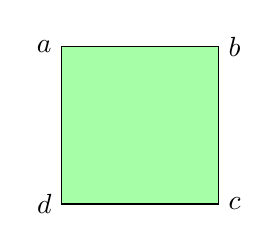
\begin{tikzpicture}[baseline=(current  bounding
				box.center)]
				\coordinate (A0) at (0,0);
				\coordinate (A1) at (0,2);
				\coordinate (A2) at (2,2);
				\coordinate (A3) at (2,0);
				\path[fill opacity=0.7, fill=green!50] (A0) -- (A3) -- (A2) -- (A1) -- cycle;
				\draw (A0) -- (A1);
				\draw (A1) -- (A2);
				\draw (A2) -- (A3);
				\draw (A0) -- (A3);
				\draw (A0) node[anchor=east] {$d$};
				\draw (A1) node[anchor=east] {$a$};
				\draw (A2) node[anchor=west] {$b$};
				\draw (A3) node[anchor=west] {$c$};
				\end{tikzpicture}
    \caption{Veranschaulichung der Wirkung von $G$}%
    \label{fig:square}
    \end{figure}
    veranschaulichen können, sowie die Relationen
    \begin{align}
        a^2c^2 & = 2\\
        b^2d^2 & = 2
    \end{align}
    korrespondierend zu den Diagonalen im Quadrat. Durch diese geometrische
    Veranschaulichung ist klar, dass nur die Permutationen in der Diedergruppe
    \[
        D_4 = \sk{ (1234), (12)(34) } \le S_4
    \]
    die speziellere Relationen erhalten, also $G(f) \le D_4$. Tatsächlich wird
    sich später zeigen, dass dies auch die Galoisgruppe des Polynoms $X^4 -2$
    ist. Mit der jetzigen Definition ist nicht direkt einzusehen, denn es ist
    unklar, ob es noch weitere algebraische Relationen gibt. Um dies effizient
    beantworten zu können, werden wir nun eine abstraktere Definition der
    Galoisgruppe geben.
\end{exa}

\section{Körpererweiterungen}%
\label{sec:korpererweiterungen}

\index{Unterkörper!Definition}Sei $L$ ein Körper. Ein \emph{Unterkörper} $K \subset L$ ist eine Teilmenge,
die $0$ und $1$ enthält und mit der von $L$ eingeschränkten Addition und
Multiplikation einen Körper bildet. Wir sagen für einen gegebenen Teilkörper $K
\subset L$ auch, dass $L/K$ eine \emph{Körpererweiterung} ist. Insbesondere ist
dann $L$ ein $K$-Vektorraum und wir nennen
\[
    [L:K] = \dim_K L
\]
den Grad von $L/K$.\index{Körpererweiterung!Grad} Eine Körpererweiterung $L/K$ heißt \emph{endlich}, falls
der Grad $[L:K]$ endlich ist.

\begin{lem}\index{Gradsatz für Körpertürme}
    \label{lem:grad}
    Seien $M/L$ und $L/K$ Körpererweiterungen. Dann ist $M/K$ endlich genau
    dann wenn $M/L$ und $L/K$ endlich sind, und in diesem Falle gilt
    \[
        [M:K] = [M:L][L:K].
    \]
\end{lem}
\begin{proof}
    Seien Teilmengen $P=\{m_1, ..., m_r\} \subset M$ und $Q=\{l_1, ..., l_s \} \subset L$ gegeben und betrachte die Teilmenge 
    \[
        QP = \{l_i m_j\; | \; 1 \le i \le s, 1 \le j \le r\}.
    \]
    Die Behauptungen folgen nun direkt aus den folgenden Aussagen. 
    \begin{enumerate}
        \item Sei $P$ linear unabhängig über $L$ und $Q$ linear unabhängig über
            $K$, dann ist $QP$ linear unabhängig über $K$.
        \item Sei $P$ erzeugend über $L$ und $Q$ erzeugend über
            $K$, dann ist $QP$ erzeugend über $K$.
    \end{enumerate}
    Diese folgen wiederum direkt aus der Umformung
    \[
        \sum_{i,j} \lambda_{i,j} l_i m_j = \sum_j ( \sum_{i} \lambda_{i,j} l_i ) m_j .
    \]
\end{proof}

\begin{exas}
    \label{exas:label}
    \begin{enumerate}
        \item $\CC/\RR$ ist eine Körpererweiterung vom Grad $2$.
        \item $\RR/\QQ$ ist eine Körpererweiterung von unendlichem Grad, z.B.
            ist $\{1,\pi, \pi^2, ... \} \subset \RR$ linear unabhängig über
            $\QQ$ (von Lindemann, 1882).
        \item Sei $K$ ein Körper und $K(X) = (K[X] \setminus \{0\})^{-1} K[X]$
            Körper der Brüche, genannt \emph{Körper der rationalen Funktionen}.\index{Körper der rationalen Funktionen!Definition}
            Dann ist $K(X)/K$ Körpererweiterung mit $[K(X):K] = \infty$. Z.B.
            ist die Menge $\{1,X,X^2, ... \}$ linear unabhängig über $K$. 
        \item Sei $f(X) \in \QQ[X]$ ein Polynom vom Grad $n \ge 1$ mit
            Nullstellen $\lambda_1, ..., \lambda_n \in \CC$. Sei $\QQ(f)$ das Bild
            des Ringhomomorphismus
            \[
                \phi: \QQ[X_1, ..., X_n] \to \CC,\; f(X_1, ..., X_n) \mapsto f(\lambda_1, ..., \lambda_n).
            \]
            Dann ist $\QQ(f)/\QQ$ eine endliche
            Körper(!)erweiterung (vom Grad $\le n^n$) (!).
    \end{enumerate}
\end{exas}

\section{Körperautomorphismen}%
\label{sec:korperautomorphismen}

\index{Körperautomorphismus!Definition}
Sei $L$ ein Körper. Einen bijektiven Ringhomomorphismus $\sigma: L \to L$
nennen wir auch \emph{Körperautomorphismus von $L$} und bezeichnen die Menge
der Körperautomorphismen von $L$ mit $\Aut(L)$. Für eine Körpererweiterung
$L/K$ bezeichnen wir
\[
    G(L/K) := \{ \sigma \in \Aut(L)\; |\; \forall x \in K: \sigma(x) = x \} \le
    \Aut(L).
\]

\begin{exa}
    \label{exa:galois}
    Sei $f \in \QQ[X]$ ein Polynom und $\QQ(f)/\QQ$ die Körpererweiterung aus
    Beispiel \ref{exas:label}. Dann gilt (!)
    \[
        G(\QQ(f)/\QQ) \cong G(f).
    \]
\end{exa}

\begin{thm}\blue{[Lemma von Artin]}\index{Lemma von Artin}
    \label{thm:galoisbound}
    Sei $L/K$ eine Körpererweiterung. Dann gilt
    \[
        | G(L/K) | \le [L:K].
    \]
\end{thm}

Für den Beweis des Satzes benötigen wir etwas Vorarbeit. 

\begin{lem}[Dedekind-Lemma]\index{Lemma von Dedekind}
    \label{lem:dedekind}
    Seien $L$ und $E$ Körper, 
    \[
        \sigma_i: L \to E  \quad , 1 \le i \le n
    \]
    paarweise verschiedene Ringhomomorphismen und $\lambda_i \in E$, $1 \le i \le n$, mit
    \begin{equation}
        \label{eq:linearchar}
        \sum_{i=1}^n \lambda_i \sigma_i = 0 \in \Abb(L,E).
    \end{equation}
    Dann gilt für alle $1 \le i \le n$: $\lambda_i = 0$. Hierbei ist die Formel
    \eqref{eq:linearchar} im $E$-Vektorraum $\Abb(L,E)$ aller Abbildungen von
    $L$ nach $E$ zu interpretieren.
\end{lem}
\begin{proof}
    Wir beweisen die Aussage durch Induktion nach $n$. Für $n =1$ folgt aus
    \eqref{eq:linearchar} direkt $0 = \lambda_1 \sigma_1(1) = \lambda_1$. Sei
    also $n >1$. Wir nehmen an, es gibt eine nichttriviale Linearkombination
    wie in \eqref{eq:linearchar} und führen die Aussage zum Widerspruch. Sei also 
    \[
        \sum_{i=1}^n \lambda_i \sigma_i = 0
    \]
    mit o.E. $\lambda_1 \ne 0$. Wir wählen $a \in L$ mit $\sigma_1(a) \ne
    \sigma_n(a)$. Dann gilt, für alle $x \in L$:
    \[
        0 = \sum_{i=1}^n \lambda_i \sigma_i(ax) - \sigma_n(a) \sum_{i=1}^n
        \lambda_i \sigma_i(x) = \sum_{i=1}^{n-1} \lambda_i(\sigma_i(a) -
        \sigma_n(a)) \sigma_i(x)
    \]
    also eine kürzere Linearkombination der $\sigma_1, ..., \sigma_{n-1}$ zu
    $0$, welche nichttrivial ist, denn $\lambda_1(\sigma_1(a) - \sigma_n(a))
    \ne 0$ per Konstruktion. Ein Widerspruch.
\end{proof}

\begin{thm}
    \label{thm:dedekind}
    Seien $L/K$ und $E/K$ Körpererweiterungen und $\sigma_1, ..., \sigma_n$
    paarweise verschiedene Ringhomomorphismen $\sigma_i: L \to E$ mit
    $\sigma_i|K = \id$. Dann gilt:
    \[
        n \le [L:K]
    \]
\end{thm}
\begin{proof}
    Für $[L:K] = \infty$ ist die Aussage inhaltslos, sei also $[L:K] =m$
    endlich und sei $l_1, ..., l_m \in L$ eine $K$-Basis von $L$. Falls $n > m$, dann existiert 
    \[
        0 \ne (\lambda_1, \lambda_2, ..., \lambda_n) \in E^n
    \]
    so dass
    \[
        \mat{ \sigma_1(l_1) & \cdots & \sigma_n(l_1)\\ \vdots & & \vdots \\ \sigma_1(l_m) & \cdots & \sigma_n(l_m) } \mat{ \lambda_1 \\ \vdots \\ \lambda_n } = 0
    \]
    Doch da $\{l_i\}$ eine Basis bildet, folgt daraus $\sum_{i=1}^n \lambda_i
    \sigma_i = 0$. Doch dies steht im Widerspruch zum Dedekind Lemma
    \ref{lem:dedekind}.
\end{proof}

Der Satz \ref{thm:galoisbound} folgt natürlich sofort aus Satz \ref{thm:dedekind} mit $L = E$. 

\section{Galoiserweiterungen}%
\label{sec:galoiserweiterungen}

\begin{defi}\index{Galoiserweiterung!Definition}
    \label{defi:galois}
    Eine endliche Körpererweiterung $L/K$ heißt \emph{Galoiserweiterung}, oder
    auch \emph{galoissch}, falls gilt:
    \[
        |G(L/K)| = [L:K].
    \]
\end{defi}

Sei $L$ ein Körper und $G \le \Aut(L)$ eine Gruppe von Körperautomorphismen von $L$. Wir nennen den Unterkörper (!)
\[
    L^G := \{ l \in L \; |\; \text{für alle $\sigma \in G$: $\sigma(l) = l$} \} \subset L
\]
den \emph{Fixkörper von $G$}.\index{Körperautomorphismus!Fixkörper}

\begin{thm}
    \label{thm:fix}
    Sei $L/K$ eine Galoiserweiterung mit Galoisgruppe $G = G(L/K)$. Dann gilt:
    \[
        L^G = K.
    \]
\end{thm}
\begin{proof}
    Es folgt aus den Definitionen, dass gilt $G(L/K) = G(L/L^G)$. Weiterhin gilt
    \[
        K \subset L^G \subset L
    \]
    Daher gilt einerseits, da $L/K$ galoissch, $|G| = [L:K]$ und andererseits,
    wegen Satz \ref{thm:galoisbound}, $|G| \le [L:L^G]$, also letztlich wegen
    Lemma \ref{lem:grad} auch $[L^G:K] = 1$. Daraus folgt (!) nun aber sofort
    $L^G = K$. 
\end{proof}

\begin{thm}[Artin]\index{Satz von Artin}
    \label{thm:artin} Sei $L$ ein Körper und $G \le \Aut(L)$. Dann gilt
    \[
        [L:L^G] = |G|.
    \]
    Insbesondere ist also, für $G$ endlich, die Körpererweiterung $L/L^G$
    galoissch mit Galoisgruppe $G$.  
\end{thm}
\begin{proof}
    Wir setzen $K = L^G$. Wegen $G \le G(L/L^G)$ gilt
    \[
        |G| \le |G(L/L^G)| \le [L:L^G]
    \]
    wobei die letzte Ungleichung aus Satz \ref{thm:galoisbound} folgt. Es
    genügt also zu zeigen: $[L:L^G] \le |G|$. Sei o.E. $|G| = n < \infty$, denn
    sonst ist die Aussage inhaltslos. Wir zeigen nun, dass je $n+1$ Elemente
    $x_1, ..., x_{n+1} \in L$ linear abhängig über $K$ sind. Betrachte dazu,
    für $G = \{\sigma_1, ..., \sigma_n\}$ das $L$-lineare Gleichungssystem
    \begin{equation}
        \label{eq:lgsgalois}
        \sum_{j=1}^{n+1} Y_j \sigma_i(x_j) = 0, \quad 1 \le i \le n
    \end{equation}
    in den Variablen $Y_1, ..., Y_{n+1}$. Dieses hat $n$ Gleichungen und $n+1$ Unbekannte, also gibt es eine nichttriviale Lösung
    \[
        0 \ne (\lambda_1, ..., \lambda_{n+1}) \in L^{n+1}
    \]
    wobei wir o.E. annehmen: $\lambda_1 \ne 0$. Für $1 \le i \le n$, wenden wir
    $\sigma_i^{-1}$ auf die $i$te Gleichung von \eqref{eq:lgsgalois} an und
    erhalten
    \[
        \sum_{j=1}^{n+1} \sigma_i^{-1}(\lambda_j) x_j = 0
    \]
    Eine Summation über alle so erhaltenen Gleichungen ergibt:
    \begin{equation}
        \label{eq:lineardep}
        \sum_{j=1}^{n+1} \alpha_j x_j = 0
    \end{equation}
    mit 
    \[
        \alpha_j = \sum_{i=1}^{n} \sigma_i^{-1}(\lambda_j) = \sum_{\sigma \in G} \sigma(\lambda_j) \in L^G = K.
    \]
    Wegen dem Dedekind Lemma gilt $\sum_{\sigma \in G} \sigma \ne 0$, so dass
    es also ein $0 \ne l \in L$ gibt mit $\sum_{\sigma \in G}\sigma(l) \ne 0$.
    Indem wir nun die Lösung $(\lambda_1, ..., \lambda_n)$ durch die Skalierung 
    \[
        (l\lambda_1^{-1} \lambda_1, ..., l\lambda_1^{-1} \lambda_{n+1})
    \]
    mit dem Skalarfaktor $l\lambda_1^{-1}$ ersetzen, erreichen wir $\alpha_1
    \ne 0$, so dass also \eqref{eq:lineardep} eine nichttriviale
    $K$-Linearkombination der Elemente $\{x_j\}$ ist. 
\end{proof}

\begin{cor}
    \label{cor:galdivides}
    Sei $L/K$ eine endliche Körpererweiterung. Dann gilt
    \[
        |G(L/K)| | [L:K].
    \]
\end{cor}
\begin{proof}
    Es gilt
    \[
        [L:K] = [L : L^G] [L^G:K]
    \]
    wobei nach dem Satz von Artin gilt: $[L:L^G] = |G|$. 
\end{proof}

\section{Die Galoiskorrespondenz}%
\label{sec:die_galoiskorrespondenz}

Für eine Körpererweiterung $L/K$ bezeichnen wir mit
\[
    \eU(G) := \{ H \; | H \le G\; \;\text{Untergruppe}\}
\]
die Menge der Untergruppen von $G$ sowie mit
\[
    \eZ(L/K) := \{ M \; | K \subset M \subset L\; \;\text{Zwischenkörper}\}
\]
die Menge der {\em Zwischenkörper von $L/K$} also Unterkörper $M \subset L$ mit $K \subset M$. 

\begin{thm}[Galoiskorrespondenz]\index{Hauptsatz der Galois-Theorie}
    \label{thm:hauptsatz}
    Sei $L/K$ eine Galoiserweiterung mit Galoisgruppe $G=G(L/K)$. Dann sind die Abbildungen
    \[
         \phi: \eU(G) \to \eZ(L/K), \; H \mapsto L^H
    \]
    und 
    \[
         \psi: \eZ(L/K) \to \eU(G), \; M \mapsto G(L/M)
    \]
    zueinander inverse Bijektionen.
\end{thm}

\begin{proof}
    Nach dem Satz von Artin (Satz \ref{thm:artin}) gilt $G(L/L^H) = H$, also
    $\psi \circ \phi = \id$, so dass insbesondere $\phi$ injektiv ist. Es
    verbleibt also zu zeigen, dass $\phi$ surjektiv ist. Dazu nehmen wir an, es
    gibt einen Zwischenkörper $K \subset M \subset L$, der nicht im Bild von
    $\phi$ liegt und führen dies zum Widerspruch.\\

    \noindent
    \emph{Schritt 1.} Zunächst wählen wir einen Zwischenkörper $K \subset M
    \subset L$ mit $M \notin \Bild(\phi)$ und $\dim_K(M)$ minimal. Insbesondere
    gilt also für jeden echten Teilkörper $K \subset M' \subsetneq M$, dass $M'
    \in \Bild(\phi)$.\\

    \noindent
    \emph{Schritt 2.} Wir wählen nun $H \le G$ minimal mit der Eigenschaft $L^H
    \subset M$, es gilt also für alle echten Untergruppen $H' \lneq H$: $L^{H'}
    \not \subset M$. Ein solches $H$ existiert, denn $L^G = K \subset M$. Indem
    wir nun $G$ durch $H$ und $K$ durch $L^H$ ersetzen, können wir ohne
    Einschränkung annehmen, dass $M/K$ keine echten Zwischenkörper enthält.\\

    \noindent
    \emph{Schritt 3.} Wir wählen weiter $\alpha \in M \setminus K$ und 
    betrachten das Bild $K[\alpha]$ des Evaluationshomomorphismus
    \[
        K[X] \to M,\; f(X) \mapsto f(\alpha).
    \]
    Dann ist $K[\alpha]$ ein endlich--dimensionaler $K$-Vektorraum und für
    jedes $0 \neq x \in K[\alpha]$ ist die Multiplikationsabbildung auf
    $K[\alpha]$ eine injektive $K$-lineare Abbildung (denn $M$ ist ein Körper),
    und daher aus Dimensionsgründen auch surjektiv. Demnach ist also $K[\alpha]
    \subset M$ ein Unterkörper so dass wegen unserer Annahme aus Schritt 2
    gilt: $K[\alpha] = M$.\\ 

    \noindent
    \emph{Schritt 4.} Wir betrachten den Stabilisator
    \[
        G_{\alpha} = \{ \sigma \in G \; | \; \sigma(\alpha) = \alpha \} \le G.
    \]
    Es gilt 
    \[
        K \subset K[\alpha] \subset L^{G_{\alpha}}
    \]
    und weiter
    \begin{equation}
        \label{eq:bahnartin}
        [L^{G_{\alpha}}:K] = \frac{[L:K]}{[L:L^{G_{\alpha}}]} = \frac{|G|}{|G_{\alpha}|} = |G.\alpha|
    \end{equation}
    wobei wir hier den Satz von Artin und die Bahnformel anwenden.\\

    \noindent
    \emph{Schritt 5.} Unter den Einschränkungen 
    \[
        \sigma|M : M \to L
    \]
    von Automorphismen $\sigma \in G(L/K)$ gibt es mindestens $|G.\alpha|$
    verschiedene Homomorphismen, denn diese bilden jeweils $\alpha$ auf
    $\sigma(\alpha)$ ab. Aus Satz \ref{thm:dedekind} folgt also
    \begin{equation}
        \label{eq:dedekindrest}
        |G.\alpha| \le [M:K].\\[1ex]
    \end{equation}

    \noindent
    \emph{Schritt 6.} Aus \eqref{eq:bahnartin} und \eqref{eq:dedekindrest}
    folgt nun aber $[L^{G_{\alpha}}:K] = [M:K]$ (denn $M \subset
    L^{G_{\alpha}}$) und daher $L^{G_{\alpha}} = M$, also $M \in \Bild(\phi)$. Ein Widerspruch.
\end{proof}

\begin{rem}
    \label{rem:galoisordnung}
    Die Mengen $\eU(G)$ und $\eZ(L/K)$ aus Satz \ref{thm:hauptsatz} sind
    partiell geordnete (gegeben durch $\subset$). Diese partielle Ordnung wird
    durch die Galoiskorrespondenz umgekehrt, es gilt also für Untergruppen
    $H_1,H_2 \le
    G$:
    \[
        H_1 \le H_2 \quad \iff \quad L^{H_2} \subset L^{H_1}.
    \]
\end{rem}

Wir untersuchen nun weitere Eigenschaften der Galoiskorrespondenz. 

\begin{thm}
    \label{thm:galoisnormal}
    Sei $L/K$ eine Galoiserweiterung mit Galoisgruppe $G=G(L/K)$ und sei $H \le
    G$ eine Untergruppe. Dann gelten:
    \begin{enumerate}
        \item Es gibt genau $(G:H)$ verschiedene Ringhomomorphismen (Körpereinbettungen) 
            \[
                \tau: L^H \to L
            \]
            mit der Eigenschaft $\tau|K = \id_K$. Für jede dieser Einbettungen
            gibt es einen Automorphismus $\sigma \in G$ so dass $\tau = \sigma|L^H$. 
        \item Für $\sigma \in G$ gilt
            \[
                \sigma(L^H) = L^{\sigma H \sigma^{-1}}, 
            \]
            der Bildkörper $\sigma(L^H)$ ist also der Fixkörper der zu $H$
            konjugierten Untergruppe $\sigma H \sigma^{-1}$. 
        \item Die Körpererweiterung $L^H/K$ ist galoissch genau dann wenn $H
            \no G$ eine normale Untergruppe ist. In diesem Falle definiert die
            Einschränkungsabbildung
            \[
                \rho: G \to G(L^H/K), \sigma \mapsto \sigma|L^H
            \]
            einen surjektiven Gruppenhomomorphismus mit Kern $H$, es gilt also insbesondere
            \[
                G(L^H/K) \cong G/H.
            \]
    \end{enumerate}
\end{thm}
\begin{proof}
    (1) Wir bezeichnen mit $\eE$ die Menge der Ringhomomorphismen $\tau: L^H \to L$
    mit $\tau|K = \id$. Die Galoisgruppe $G$ operiert auf $\eE$ via
    \[
        \sigma.\tau = \sigma \circ \tau.
    \]
    Der Stabilisator der Inklusionseinbettung $\iota: L^H \subset L$ ist, nach dem
    Satz von Artin, genau $H$. Daher gilt:
    \[
        (G:H) = |G.\iota| = |\{\tau \in \eE\; \left| \; \text{$\tau = \sigma|L^H$ für ein $\sigma \in G$} \right. \}| \le |\eE|
    \]
    Andererseits gilt nach Satz \ref{thm:dedekind} 
    \[
        |\eE| \le [L^H:K] = \frac{[L:K]}{[L:L^H]} = \frac{|G|}{|H|} = (G:H).
    \]

    \noindent
    (2) Für $\sigma \in G$, $\gamma \in H$ und $x \in L$ gilt
    \[
        \gamma(x) = x \quad \iff \quad \sigma\gamma\sigma^{-1}(\sigma(x)) = \sigma(x).
    \]

    \noindent
    (3) Nach (1) gilt
    \[
        |\eE| = [L^H:K].
    \]
    Die Abbildung
    \[
        \epsilon:  G(L^H/K) \to \eE, \alpha \mapsto \iota \circ \alpha
    \]
    definiert eine Injektion, so dass also gilt: $|G(L^H/K)| \le |\eE| = [L^H:K]$. Demnach ist die Erweiterung $L^H/K$
    galoissch genau dann wenn die Abbildung $\epsilon$ eine Bijektion
    ist, wenn also für jede der Einbettungen aus $\tau \in \eE$ gilt $\tau(L^H)
    = L^H$. Da nach (1) die Einschränkungsabbildung eine Surjektion $G \to \eE$
    definiert, ist dies wegen (2) und Satz \ref{thm:hauptsatz} äquivalent zur Bedingung
    \[
        \forall \sigma \in G: \sigma H \sigma^{-1} = H
    \]
    also $H \no G$ normal. In diesem Falle definiert also, für jedes $\sigma \in
    G$, die Einschränkung $\sigma|L^H$ einen Automorphismus von $L^H$, so dass
    wir einen wohldefinierten surjektiven Homomorphismus 
    \[
        G \to G(L^H/K), \; \sigma \mapsto \sigma|L^H
    \]
    mit Kern $G(L/L^H) = H$ erhalten.
\end{proof}

\begin{rem}\index{Hauptsatz der Galois-Theorie!Interpretation}
    \label{rem:galoisoperation}
    Die verfeinerten Eigenschaften der Galoiskorrespondenz aus Satz
    \ref{thm:galoisnormal} lassen sich sehr einprägsam wie folgt
    interpretieren: 

    Die Galoiskorrespondenz definiert eine kanonische Bijektion
    zwischen der Menge $\eU(G)$ der Untergruppen von $G$ und der Menge
    $\eZ(L/K)$ von Zwischenkörpern von $L/K$. Beide Mengen sind mit natürlichen
    Wirkungen der Gruppe $G$ ausgestattet: $G$ operiert auf $\eU(G)$ via
    Konjugation, also $\sigma.H = \sigma H \sigma^{-1}$, und auf $\eZ(L/M)$ via
    $\sigma.M = \sigma(M)$. 
    Satz \ref{thm:galoisnormal} impliziert nun, dass die Galoiskorrespondenz eine 
    \emph{$G$-äquivariante} Bijektion ist, die also die beiden $G$-Wirkungen
    ineinander überführt: 
    \[
        G \actson \eU(G) \quad \overset{\cong}{\longleftrightarrow} \quad \eZ(L/K) \actsonright G
    \]
    Die Fixpunkte dieser $G$-Wirkungen entsprechen
    einerseits den normalen Untergruppen von $G$ und andererseits den
    Galoiserweiterungen von $K$. Allgemeiner entsprechen die Bahnen der
    $G$-Wirkung auf $\eU(G)$ Konjugationsklassen von Untergruppen, welche über
    die Galoiskorrespondenz mit $G$-Bahnen in $\eZ(L/K)$ identifiziert werden.
    Diese entsprechen (!) Isomorphieklassen von Zwischenkörpern über $K$. 
\end{rem}

\begin{prob}\index{Untergruppe!Normalisator}
    \label{prob:verfeinerung}
    Sei $L/K$ eine Galoiserweiterung mit Galoisgruppe $G(L/K)$ und $H \le G$
    eine Untergruppe mit zugehörigem Zwischenkörper $M = L^H$. Wir definieren
    die Normalisatoruntergruppe 
    \[
        \N_G(H) = \{ \sigma \in G \; | \; \sigma H \sigma^{-1} = H \} \le G
    \]
    von $H$ in $G$. Dann gelten:
    \begin{enumerate}
        \item Die Inklusionsabbildung $G(M/K) \subset G(M/L^{\N_G(H)})$ ist ein Isomorphismus. 
        \item Die Untergruppe $H \le \N_G(H)$ ist normal und die
            Körpererweiterung $M/L^{\N_G(H)}$ ist galoissch mit Galoisgruppe
            $\N_G(H)/H$. 
        \item Sei $\eZ_M$ die Menge der zu $M$ über $K$ isomorphen
            Zwischenkörper von $L/K$. Dann gilt: 
            \[
                |\eZ_M| = (G:\N_G(H)).
            \]
        \item Folgere, dass insbesondere gilt
            \[
                (G:H) = |\eZ_M| |G(M/K)|.
            \]
    \end{enumerate}
\end{prob}

\begin{exa}
    \label{exa:label}
    Sei $L/K$ eine Galoiserweiterung mit Galoisgruppe $G(L/K) \cong S_3$. In \S
    \ref{sub:zerfallungskorper} werden wir sehen, dass die Erweiterung
    $\QQ(f)/\QQ$ für $f(X) = X^3 - 2$ ein Beispiel für eine solche
    Erweiterung ist. Nach der Galoiskorrespondenz entspricht der partiell
    geordneten Menge von Untergruppen
    \[
    \begin{tikzcd}
        & &S_3  & & \\
        & & & & A_3 \ar[ull,dash]\\
        C \ar[uurr,dash] & C'\ar[uur,dash] & C''\ar[uu,dash] &   \\
        & & \{ (1) \}\ar[ull,dash]\ar[ul,dash]\ar[u,dash]\ar[uurr,dash]&  & 
    \end{tikzcd}
    \]
    von $S_3$, mit $C = \sk{(12)}$, $C' = \sk{(23)}$, $C'' = \sk{(13)}$, die Menge von Zwischenkörpern
    \[
    \begin{tikzcd}
        & &K  & & \\
        & & & & L^{A_3} \ar[ull,dash]\\
        L^{C}\ar[uurr,dash] & L^{C'}\ar[uur,dash] & L^{C''} \ar[uu,dash] &   \\
        & & L\ar[ull,dash]\ar[ul,dash]\ar[u,dash]\ar[uurr,dash]&  & 
    \end{tikzcd}
    \]
    von $L/K$. Dabei ist die Erweiterung $L^{A_3}/K$ galoissch mit Galoisgruppe
    $S_3/A_3 \cong C_2$. Die restlichen Zwischenkörper $L^C$, $L^{C'}$ und
    $L^{C''}$ sind nicht galoissch: Die zugehörigen Gruppen $C$, $C'$ und
    $C''$ sind kongugiert so dass die Zwischenkörper $L^C$, $L^{C'}$ und
    $L^{C''}$ also isomorph über $K$ sind. Vom Standpunkt der $G$-Wirkungen aus
    Bemerkung \ref{rem:galoisoperation} wirkt die Gruppe $S_3$ mit Fixpunkt
    $A_3$ (bzw. $L^{A_3}$) und durch zyklische Permutation der Untergruppen
    Gruppen $C$, $C'$ und $C''$ (bzw. $L^C$, $L^{C'}$ und $L^{C''}$).
\end{exa}

\section{Zerfällungskörper}%
\label{sub:zerfallungskorper}

\begin{defi}\index{Zerfällungskörper!Definition}
    \label{defi:zerfällung}
    Sei $K$ ein Körper und $f \in K[X]$ ein Polynom. Ein Körper $E$ mit $K \subset E$ heißt {\em Zerfällungskörper} von $f$ falls
    \begin{enumerate}
        \item $f = c (X - \alpha_1)(X- \alpha_2) \cdots (X - \alpha_n) \in E[X]$,
        \item $E = K(\alpha_1, ..., \alpha_n)$,
    \end{enumerate}
    wobei 
    \[
        K(\alpha_1, ..., \alpha_n) := \bigcap_{ \substack{ L \in \eZ(E/K)\\ \{\alpha_1, ..., \alpha_n \} \subset L } } L.
    \]
\end{defi}

\begin{thm}\index{Zerfällungskörper!Existenz und Eindeutigkeit}
    \label{thm:zerfexun}
    Sei $K$ ein Körper und $f \in K[X]$ ein Polynom. Dann existiert ein
    Zerfällungskörper von $f$ und ist bis auf Körperisomorphie über $K$
    eindeutig bestimmt.
\end{thm}
\begin{proof}
    Wir zeigen zunächst die Existenz. Für eine Körpererweiterung $L/K$, die eine Nullstelle $\alpha \in L$ von $f$ enthält, gilt
    \[
        f(X) = (X-\alpha) g(X) \in L[X]
    \]
    für $g(X) \in L[X]$ mit $\grad(g(X)) < \grad(f(X))$. Es genügt also für
    allgemeines $K$ und $f$ einen Körper $L/K$ zu konstruieren der eine
    Nullstelle von $f$ enthält (denn dann kann diese Konstruktion iteriert
    werden, bis $f$ vollständig in Linearfaktoren zerfällt). Ohne Einschränkung
    können wir hierbei annehmen, dass $f$ irreduzibel ist (indem wir die
    Konstruktion auf einen Primfaktor von $f$ anwenden). In diesem Fall erhalten wir mit
    \begin{equation}
        \label{eq:primitiv}
        L := K[T]/(f(T))
    \end{equation}
    einen Körper der die Nullstelle $\alpha = [T]$ von $f$ enthält.
    Körpererweiterungen der Form $L/K$ wie in \eqref{eq:primitiv} nennen wir
    auch {\em primitive} Erweiterungen. Durch die oben angedeutete sukzessive
    Anwendung dieser Konstruktion ergibt sich also ein Turm
    \[
        K \hra L_1 \hra L_2 \hra ... \hra L_m
    \]
    von primitiven Körpererweiterungen wobei $L_m$ ein Zerfällungskörper ist
    (!). Zum Beweis der Eindeutigkeit benötigen wir noch ein vorbereitendes Lemma.
\end{proof}

Für eine Körpereinbettung $\phi: L \hra E$ und
\[
    f(X) = a_n X^n + a_{n-1} X^{n-1} + ... + a_0 \in L[X]
\]
definieren wir
\begin{equation}
    \label{eq:hochphi}
    f^{\phi}(X) := \phi(a_n) X^n + \phi(a_{n-1}) X^{n-1} + ... + \phi(a_n) \in E[X].
\end{equation}
Durch direktes Nachrechnen folgt, dass die Abbildung
\begin{equation}\label{eq:koeff}
    L[X] \to E[X], f(X) \mapsto f^{\phi}(X)
\end{equation}
ein Ringhomomorphismus ist. 

\begin{lem}
    \label{lem:primitive}
    Sei $\phi: L \hra E$ eine Körpereinbettung, $f(X) \in L[X]$ irreduzibel,
    und $\alpha \in E$ eine Nullstelle von $f^{\phi}(X)$. Dann gibt es eine
    eindeutig bestimmte Körpereinbettung
        \[
        \begin{tikzcd}
            L[X]/(f(X)) \ar[hook]{rr}{\psi} & &E\\
                                                 & L\ar{ul}{\subset} \ar{ur}{\phi} & 
        \end{tikzcd}
        \]
        so dass $\phi(X) = \alpha$. 
\end{lem}
\begin{proof}
    Betrachte zunächst den Ringhomomorphismus
    \[
       {\xi}: L[X] \to E, g \mapsto g^\phi(\alpha)
    \]
    definiert als die Komposition von \eqref{eq:koeff} mit dem
    Evaluationshomomorphismus. Dann gilt 
    \[
        (f(X)) \subset \Kern(\xi) \subsetneq L[X]
    \]
    Da aber $\widetilde{f(X)}$ irreduzibel ist, ist $(f(X))$ maximal so dass
    also gilt $(f(X)) =  \Kern(\widetilde{\psi})$. Daher erhalten wir den
    gewünschten Homomorphismus als
    \[
        \phi := \bar{\xi}: L[X]/(f(X)) \to E.
    \]
\end{proof}

\begin{proof}[Beweis der Eindeutigkeit des Zerfällungskörpers.]
    Sei 
    \[
        K \hra L_1 \hra L_2 \hra \cdots \hra L_m
    \]
    der im Existenzbeweis konstruierte Zerfällungskörper von $f(X)$ und $E/K$
    ein beliebiger Zerfällungskörper mit $L_{i+1} = L_i[X]/(f_i(X))$ für
    $f_i(X) \in L_i[X]$ irreduzibel. Wir behaupten, dass sich die
    Inklusionsabbildung $\phi_0: K \to E$ zu einer Folge $\phi_i: L_i \hra E$
    von Einbettungen fortsetzen lässt, so dass gilt: $\phi_{i+1}|L_i = \phi_i$.
    Wir beweisen dies induktiv, mit folgendem Induktionsschritt: 
    \[
        \begin{tikzcd}
            L_i[X]/(f_i(X)) \ar[hook, dashed]{rr}{\phi_{i+1}} & &E\\
            & L_i\ar{ul}{\subset} \ar{ur}{\phi_i} & 
        \end{tikzcd}
    \]
    wobei es für die Existenz von $\phi_{i+1}$ nach Lemma \ref{lem:primitive}
    ausreicht zu zeigen, dass das Polynom $f_i^{\phi_i}(X) \in E[X]$ eine
    Nullstelle besitzt. Es gilt
    \[
        f(X) = f_i(X) g(X) \in L_i[X]
    \]
    mit $f_i(X)$ irreduzibel und demnach auch 
    \[
        f(X) = f^{\phi_i}(X) = f_i^{\phi_i}(X) g^{\phi_i}(X) \in E[X].
    \]
    Da $E$ ein Zerfällungskörper ist, zerfällt $f(X)$ in Linearfaktoren
    (Primfaktoren) und daher auch $f_i^{\phi_i}(X)$ (und auch $g^{\phi_i}(X)$), also
    \[
        f_i^{\phi_i}(X) = b (X-\beta_1) \cdots (X - \beta_k)
    \]
    so dass die Elemente $\beta_1, ..., \beta_k \in E$ Nullstellen von
    $f_i^{\phi_i}(X)$ sind.  Schließlich gilt zudem, dass die Inklusion
    $\phi_n: L_n \hra E$ surjektiv ist, denn in $L_m[X]$ gilt
    \[
        f(X) = c (X - \alpha_1) (X-\alpha_2) \cdots (X-\alpha_m)  \in L_n[X]
    \]
    und somit 
    \[
        f(X) = f^{\phi_m}(X) = \phi_m(c) (X - \phi_m(\alpha_1)) (X- \phi_m(\alpha_2)) \cdots (X- \phi_m(\alpha_n)) \in E[X].
    \]
    Daher enthält das Bild von $\phi_m$ alle Nullstellen $\phi_m(\alpha_1), ..., \phi_m(\alpha_n) \in E$ von $f(X)$ in $E$, und daher 
    \[
        E = K(\phi_m(\alpha_1), ..., \phi_m(\alpha_n)) \subset \Bild(\phi_n). 
    \]
\end{proof}

\begin{exa}
    \label{exa:x42}
    Sei $f(X) = X^4 - 2 \in \QQ[X]$. Ein Zerfällungskörper von $f$ lässt sich
    durch einen Turm von zwei primitiven Erweiterungen konstruieren: Zunächst
    ist 
    \[
        L = \QQ(\sqrt[4]{2}) \cong \QQ[T]/(f_1(T))
    \]
    eine primitive Erweiterung für das irreduzible Polynom $f$
    (Eisenstein Kriterium), wobei $\sqrt[4]{2} \in \CC$ die eindeutige reelle
    positive $4$te Wurzel in $\RR$ bezeichnet. Über $L$ zerlegt sich $f$ in 
    \[
        f(X) = (X - \sqrt[4]{2})(X + \sqrt[4]{2}) (X^{2} + \sqrt{2}).
    \]
    Das Polynom 
    \[
        f_1(X) = X^{2} + \sqrt{2} \in L[X] \subset \RR[X]
    \]
    ist irreduzibel, denn es hat keine reellen Nullstellen. Es definiert daher die primitive Erweiterung
    \[
        E = L[T]/(f_1(T)) \cong \QQ(\sqrt[4]{2}, i\sqrt[4]{2})
    \]
    Alternativ können wir 
    \[
        \QQ(\sqrt[4]{2}, i\sqrt[4]{2}) = \QQ(\sqrt[4]{2}, i)
    \]
    als primitive Erweiterung 
    \[
        L[S]/(S^2 + 1) 
    \]
    bezüglich des irreduziblen Polynoms $S^2 + 1 \in L[S]$ mit
    Nullstellen $\pm i \in \CC$ beschreiben. Es gilt in $E[X]$:
    \[
        f(X) = (X - \sqrt[4]{2})(X + \sqrt[4]{2}) (X - i\sqrt[4]{2})(X + i\sqrt[4]{2})
    \]
    so dass $E$ also ein Zerfällungskörper von $f$ ist. 

    Wir erhalten 
    \[
        [E: \QQ] = [E: L][L:\QQ] = 2 \cdot 4 = 8.
    \]
    Durch jeweils zweimaliges Anwenden von Lemma \ref{lem:primitive}
    konstruieren wir die folgenden Automorphismen
    $\sigma,\tau \in G := G(E, \QQ)$:
    \[
        \tau: E \to E, \begin{cases} \sqrt[4]{2} & \mapsto \sqrt[4]{2}\\ i & \mapsto -i \end{cases}
    \]

    \[
        \sigma: E \to E, \begin{cases} \sqrt[4]{2} & \mapsto i\sqrt[4]{2}\\ i & \mapsto i \end{cases}
    \]
    Zum Beispiel unter Zuhilfenahme der Veranschaulichung in Figur \ref{fig:square} sieht man ein, dass gilt
    \[
        D_4 \cong \sk{\sigma,\tau} \le G.
    \]
    Wegen Satz \ref{thm:galoisbound} gilt $|G| \le [E:\QQ] = 8$, so dass also gelten muss 
    \[
            \sk{\sigma,\tau} = G.
    \]
    Die Menge der Untergruppen $\eU(G)$ sieht wie folgt (!) aus
    \[
    \begin{tikzcd}
        8  &  & & \color{purple}G \ar[dl,dash]\ar[d,dash]\ar[dr,dash]& &\\
        4  &   & \color{purple} \sk{\sigma^2\tau,  \tau} \ar[dl,dash]\ar[d,dash]\ar[dr,dash] &\color{purple} \sk{\sigma}\ar[d,dash] & \ar[dl,dash]\ar[d,dash]\ar[dr,dash]\color{purple}\sk{\sigma\tau,  \sigma^3\tau} & \\
        2  & \sk{\sigma^2\tau} & \sk{\tau}  &\color{purple} \sk{\sigma^2} & \sk{\sigma\tau} & \sk{\sigma^3\tau}  \\
        1  &                & &\color{purple} \{1 \}\ar[ull,dash] \ar[ul,dash]\ar[u,dash]\ar[ur,dash] \ar[urr,dash]& & 
    \end{tikzcd}
    \]
    wobei in der linken Spalte die Ordnungen angegeben sind und die farbigen
    Gruppen die normalen Untergruppen kennzeichnen. Die korrespondierende Menge
    der Zwischenkörper von $E/K$ lässt sich wie folgt (!) beschreiben
    \[
    \begin{tikzcd}
        1  &  & & \color{purple}\QQ \ar[dl,dash]\ar[d,dash]\ar[dr,dash]& &\\
        2  &   &\color{purple} \QQ(\sqrt{2}) \ar[dl,dash]\ar[d,dash]\ar[dr,dash] &\color{purple} \QQ(i) \ar[d,dash] & \ar[dl,dash]\ar[d,dash]\ar[dr,dash]\color{purple}\QQ(\sqrt{-2}) & \\
        4  & \QQ(\sqrt[4]{2}) & \QQ(i\sqrt[4]{2})  &\color{purple} \QQ(\sqrt{2},i)  & \QQ(\sqrt[4]{-2}) & \QQ(i\sqrt[4]{-2})  \\
        8  &                & &\color{purple} \QQ(\sqrt[4]{2},i) \ar[ull,dash] \ar[ul,dash]\ar[u,dash]\ar[ur,dash] \ar[urr,dash]& & 
    \end{tikzcd}
    \]
    wobei in der linken Spalte der Grad der Körpererweiterungen über $\QQ$
    angegeben ist und die farbig gekennzeichneten Körper die
    Galoiserweiterungen von $\QQ$ sind. Um zu überprüfen, dass ein angegebener
    Zwischenkörper $M$ tatsächlich der Fixkörper der korrespondierenden
    Untergruppe $H$ ist zeigt man jeweils
    \begin{enumerate}[label = \arabic *.]
        \item $M \subset E^H$, und
        \item $[K:M] = (G:H)$.
    \end{enumerate}
    Diese Bedingungen implizieren $M = E^H$. Hierbei bedeuten genauer:
    \begin{align*}
        \sqrt{-2} & := i \sqrt{2}\\
        \sqrt[4]{-2} & := \frac{1+i}{\sqrt{2}}\sqrt[4]{2},
    \end{align*}
    wobei wir bemerken, dass $\zeta := \frac{1+i}{\sqrt{2}}$ eine primitive
    $8$te Einheitswurzel ist (deren Potenzen also alle $8$ten Einheitswurzeln
    durchläuft), insbesondere gilt $\zeta^4 = -1$. Es gilt weiter
    \[
        \QQ(\sqrt{2}, i) = \QQ(\zeta) 
    \]
    so dass dieser Körper also der Zerfällungskörper des Polynoms $X^8 - 1$
    ist. Unter der Galoiskorrespondenz korrespondiert $\QQ(\zeta)$ zum Zentrum
    $\sk{\sigma^2}$ von $G$. Die Galoisgruppe $G(\QQ(\zeta)/\QQ)$ ist demnach
    isomorph zu
    \[
        G/\sk{\sigma^2} \cong C_2 \times C_2.
    \]
    Die Galoisgruppen der Zerfällungskörper der Polynome $X^n -1$, der
    sogenannten {\em Kreisteilungskörper} werden wir im nachfolgenden Abschnitt
    systematischer untersuchen.
\end{exa}

\begin{defi}\index{Polynom!Separabilität}
    \label{defi:sep}
    Sei $K$ ein Körper. Ein irreduzibles Polynom $f \in K[X]$ heißt \emph{separabel}, falls in seinem Zerfällungskörper $E/K$ gilt:
    \[
        f = c (X-\alpha_1)(X-\alpha_2) \cdots (X-\alpha_k) \in E[X]
    \]
    mit paarweise verschiedenen $\alpha_i \in E$, falls also $f$ in $E$ nur
    \emph{einfache Nullstellen} hat. Im allgemeinen heißt ein Polynom in $K[X]$ \emph{separabel},
    falls jeder seiner Primfaktoren separabel ist. 
\end{defi}

\begin{thm}
    \label{thm:sepgalois}
    Sei $K$ ein Körper, $f \in K[X]$ ein separables Polynom, und $E$ ein
    Zerfällungskörper von $f$. Dann ist $E/K$ eine Galoiserweiterung. 
\end{thm}
\begin{proof}
    Der Beweis von Satz \ref{thm:zerfexun} zeigt, dass es eine Kette von
    primitiven Körpererweiterungen der Form 
    \[
        K \subset L_1 \subset L_2 \subset \cdots \subset L_n = E
    \]
    gibt. Es gilt also $L_{i+1} \cong L_i[X]/(f_i)$ für $f_i \in L_i[X]$
    irreduzibel. Zu einer gegebenen Einbettung $\phi_i: L_i \hra E$ betrachten
    wir
    \[
    \begin{tikzcd}
        L_{i+1}\ar[dashed]{r}{\phi_{i+1}} & E \\
        L_i \ar{ur}{\phi_i} \ar{u}{\subset}& .
    \end{tikzcd}
    \]
    Nach Lemma \ref{lem:primitive} gibt es für jede Nullstelle $\alpha$ von
    $f_i^{\phi_i}$ in $E$ eine Einbettung $\phi_{i+1}$ mit $\phi_{i+1}(X) =
    \alpha$. Doch $f_i$ ist Primfaktor des Polynoms $f \in L_i[X]$ und teilt
    daher (!) einen Primfaktor von $f \in K[X]$. Das Polynom $f_i$ (und damit
    auch $f_i^{\phi_i}$ besitzt also genau $\grad(f_i)$ verschiedene Nullstellen
    in $E$, so dass es daher auch genau $\grad(f_i) = [L_{i+1}:L_i]$
    verschiedene Fortsetzungen $\phi_{i+1}$ der vorgegebenen Einbettung
    $\phi_i$ gibt. 

    Sukzessive erhalten wir durch diese Konstruktion also 
    \[
        [E:L_{n-1}] [L_{n-1}:L_{n-2}] \cdots [L_1:K] = [E:K]
    \]
    verschiedene Einbettungen $L_n \hra L_n = E$, die, mit dem Argument im
    Eindeutigkeitsbeweis von Satz \ref{thm:zerfexun} auch surjektiv sind. Also gilt
    wegen Satz \ref{thm:galoisbound}
    \[
           [E:K] = |G(E/K)| 
    \]
    so dass $E/K$ galoissch ist. 
\end{proof}

Es gilt auch umgekehrt:

\begin{prob}
    \label{prob:galois}
    Jede Galoiserweiterung $E/K$ ist Zerfällungskörper eines separablen Polynoms in $K[X]$. 
\end{prob}

\index{Algebraische Ableitung!Definition}
Wir stellen nun noch ein einfaches Kriterium zum Testen der Separabilität eines Polynoms bereit. Dazu definieren wir für 
\[
    f(X) = a_n X^n + a_{n-1} X^{n-1} + ... + a_0 \in K[X]
\]
die \emph{algebraische Ableitung}
\[
    \partial f = \diff{f}{X} = n a_n X^{n-1} + (n-1) a_{n-1} X^{n-2} + ... + a_1 \in K[X].
\]
Man verifiziert durch direkte Rechnung: Für $\lambda \in K$ und $f,g \in K[X]$ gelten
\begin{align}
    \partial(\lambda f + g) & = \lambda \partial(f) + \partial(g) & \text{$K$-Linearität}\\
    \partial(fg) &= f \partial(g) + \partial(f)g & \text{Leibnizregel} \label{eq:leibniz}
\end{align}


\begin{lem}
    \label{lem:kritsimp}
    Sei $f \in K[X]$ ein Polynom, $L/K$ Körpererweiterung und $\alpha \in L$
    Nullstelle von $f$. Dann sind äquivalent:
    \begin{enumerate}[label=(\roman{*})]
        \item $\alpha$ einfach,
        \item $\partial f (\alpha) \neq 0$.
    \end{enumerate}
\end{lem}
\begin{proof}
    Die Nullstelle $\alpha$ ist einfach genau dann wenn gilt
    \[
        f(X) = (X-\alpha)g(X)
    \]
    mit $(X-\alpha) \nmid g(X)$, so dass die Behauptung sofort aus \eqref{eq:leibniz}
    \begin{equation}
        \label{eq:leibnizformel}
            \partial f = g(X) + (X-\alpha) \partial g
    \end{equation}
    folgt. 
\end{proof}

\begin{prop} \label{prop:irredsep} Sei $K$ ein Körper und sei $f \in K[X]$ ein
    irreduzibles Polynom. Dann sind äquivalent:
    \begin{enumerate}[label=(\roman *)]
        \item $f$ ist separabel.
        \item $\ggT(f, \partial f) = 1$.
        \item $\partial f \neq 0$.
    \end{enumerate}
\end{prop}
\begin{proof}
    Wir zeigen zunächst die Äquivalenz von (i) und (ii): 
    Sei $E/K$ ein Zerfällungskörper von $f$. Falls $f$ separabel ist, dann
    folgt aus \eqref{eq:leibnizformel}, dass keiner der Primfaktoren
    $(X-\alpha)$ von $f$ in $E[X]$ ein Teiler von $\partial f$ ist, also sind
    $f$ und $\partial f$ coprim.
    Seien umgekehrt $\ggT(f, \partial f) = 1$, dann gibt es also $r,s \in K[X]$ mit
    \begin{equation}
        \label{eq:ggtsep}
        rf + s\partial f = 1
    \end{equation}
    Für eine Nullstelle $\alpha \in E$ von $f$ muss dann aber $\partial f (\alpha) \neq 0$
    gelten, denn sonst impliziert Evaluation von \eqref{eq:ggtsep} bei $\alpha$
    die Gleichung $0 = 1$. 

    Nun zur Äquivalenz von (ii) und (iii): Falls (ii) gilt, dann folgt aus
    \eqref{eq:ggtsep} sofort (iii) denn sonst wäre $f$ eine Einheit in $K[X]$.
    Falls umgekehrt $\partial f \neq 0$ dann folgt, wegen $\grad(\partial f)
    < \grad(f)$ und $f$ irreduzibel, dass die einzigen gemeinsamen Teiler von
    $f$ und $\partial f$ Einheiten sind. 
\end{proof}

\begin{cor} Sei $K$ ein Körper. 
    \label{cor:charsep}
    \begin{enumerate}
        \item Falls $\charac(K) = 0$ so ist jedes Polynom $f \in K[X]$ separabel.
        \item Falls $\charac(K) = p$ so sind für ein irreduzibles Polynom $f \in K[X]$ äquivalent:
            \begin{enumerate}[label=(\roman *)]
                \item $f$ inseparabel.
                \item Es gibt $g \in K[X]$ mit $f(X) = g(X^p)$. 
            \end{enumerate}
    \end{enumerate}
\end{cor}

\begin{exa}
    \label{exa:insep}
    Sei $K$ ein Körper der Charakteristik $p > 0$ und sei $f = X^p - a \in
    K[X]$. Im Zerfällungskörper $E/K$ besitzt $f$ eine Nullstelle $\alpha \in
    E$ es gilt also $\alpha^p = a$. Dann gilt in $E[X]$:
    \[
        (X-\alpha)^p = X^p + \sum_{k=1}^{p-1} {p \choose k} X^{p-k} (-\alpha)^{k} + (- \alpha)^p = X^p - a 
    \]
    wobei $(-\alpha)^p = - \alpha^p = -a$ da $p$ entweder ungerade ist, oder $1 = -1$ in $K$. 
    Insbesondere ist also $\alpha$ eine Nullstelle mit Vielfachheit $p$ so dass
    $f$, in Übereinstimmung mit der Aussage von Korollar \ref{cor:charsep}
    inseparabel ist. 
\end{exa}


\section{Permutationsdarstellung der Galoisgruppe}%
\label{sub:permutationsdarstellung_der_galoisgruppe}

In diesem Abschnitt studieren wir die Galoisgruppe eines Polynoms über ihre
Wirkung auf den Nullstellen in einem Zerfällungskörper. 

\begin{thm}
    \label{thm:galop}
        Sei $K$ Körper, $f \in K[X]$ irreduzibel und separabel mit Leitkoeffizient $1$ und $\grad(f)
        = n$. Über dem Zerfällungskörper $E$ von $f$ gilt also
        \[
            f = (X-\alpha_1)(X-\alpha_2)\cdots (X-\alpha_n)
        \]
        wobei $A = \{ \alpha_1, ..., \alpha_n \}$ die Menge der (paarweise
        verschiedenen) Nullstellen von $f$ in $E$ bezeichnet. Sei weiter $G =
        G(E/K)$ die Galoisgruppe. Dann gelten:
        \begin{enumerate}
            \item Die Operation $G \actson E$ schränkt sich ein auf eine Operation $G \actson A$. 
            \item \index{Wirkung!treu}Die Operation $G \actson A$ ist \emph{treu}, d.h. falls für
                ein $\sigma \in G$ und für alle $\alpha_i \in A$ gilt:
                $\sigma(\alpha_i) = \alpha_i$ dann folgt schon $\sigma = \id$. 
            \item Die Operation $G \actson A$ ist \emph{transitiv}, d.h. für
                $\alpha_i \neq \alpha_j$ gibt es $\sigma \in G$ mit
                $\sigma(\alpha_i) = \alpha_j$.
        \end{enumerate}
\end{thm}
\begin{proof}
    (1) Die Galoisgruppe $G$ operiert via Ringhomomorphismen auf $E[X]$ via 
    \[
        \sigma.g(X) = g^{\sigma}(X), \quad \sigma \in G, g \in E[X]
    \]
    wobei wir die Notation \ref{eq:hochphi} verwenden. Es gilt in $E[X]$:
    \[
        \prod_{i=1}^n (X - \alpha_i) = f(X) = \sigma.f(X) = \prod_{i=1}^n (X - \sigma(\alpha_i))
    \]
    so dass $\sigma$ die Nullstellen $\alpha_1, \alpha_2, ..., \alpha_n$ wegen
    der Eindeutigkeit der Primfaktorzerlegung in $E[X]$ permutieren muss.\\

    \noindent
    (2) Jedes Element in $E$ lässt sich als ein $K$-polynomialer Ausdruck in
    den Nullstellen $\alpha_1, \alpha_2, ..., \alpha_n$ schreiben. Wenn $\sigma
    \in G$ also alle $\alpha_i$ festhält, dann gilt $\sigma = \id_E$.\\

    \noindent
    (3) Es gilt $E[X]^G = K[X]$. Falls $G \actson A$ nicht transitiv ist, dann
    zerlegt sich $A$ in Bahnen
    \[
        A = A_1 \dot{\cup} A_2 \dot{\cup} \cdots \dot{\cup} A_k
    \]
    und es gilt entsprechend
    \begin{equation}
        \label{eq:widerspruchzerlegung}
        f = f_1 f_2 \cdots f_k \in E[X]
    \end{equation}
    mit 
    \[
        f_i(X) = \prod_{\alpha \in A_i} (X - \alpha).
    \]
    Da die Wirkung von $G$ für jedes $1 \le i \le k$ die Teilmenge $A_i$
    erhält, gilt $f_i \in E[X]^G = K[X]$. Damit gilt die Zerlegung
    \eqref{eq:widerspruchzerlegung} schon in $K[X]$, ein Widerspruch zur
    Irreduzibilität von $f$. 
\end{proof}

\begin{rem}
    \label{rem:allgemeinpermutation}
    Für ein allgemeines separables Polynom $f \in K[X]$ betrachten wir die
    Primfaktorzerlegung
    \[
        f(X) = \lambda f_1(X) f_2(X) \cdots f_k(X)
    \]
    mit $f_i(X)$ irreduzbel und Leitkoeffizient $1$. Sei $E$ ein
    Zerfällungskörper von $f$. Das Argument im Beweis von Satz \ref{thm:galop} (1) 
    zeigt, dass sich die Wirkung $G \actson E$ auf eine Wirkung auf jeder der
    Nullstellenmengen $A_i$ der irreduziblen Polynome $f_i(X)$ einschränkt. Für
    $n = \grad(f)$ und $n_i = \grad(f_i)$ (also $\sum n_i = n$) erhalten wir so einen Homomorphismus
    \[
        G(E/K) \hra S_{A_1} \times S_{A_2} \times  \cdots S_{A_k} \cong S_{n_1}
        \times S_{n_2} \times \cdots \times S_{n_k} \hra S_n
    \]
    der nach dem Argument im Beweis von Satz \ref{thm:galop} (2) injektiv ist.
    Wir können also $G(E/K)$ mit einer Untergruppe von $S_n$ identifizieren und
    es gilt (Argument von Satz \ref{thm:galop} (3)) dass $f$ irreduzibel in
    $K[X]$ ist, genau dann wenn die Operation $G(E/K) \actson \{1,
    ..., n\}$ transitiv ist. 
\end{rem}

Für die Bestimmung der Galoisgruppe $G$ eines irreduziblen, separablen Polynoms
$f$ ergibt sich folgende Strategie:
\begin{enumerate}
    \item Bestimme alle transitiven Untergruppen von $S_n$.
    \item Finde für jede transitive Untergruppe $H \le S_n$ ein Kriterium um zu
        entscheiden ob $G \le H$. 
\end{enumerate}
Wir illustrieren dies am Beispiel der transitiven Untergruppe 
\[
    A_n \le S_n.
\]

\begin{defi}\index{Polynom!Diskriminante}
    \label{defi:diskriminante}
    Sei $K$ ein Körper und $f \in K[X]$ ein irreduzibles separables Polynom vom Grad $n$. Sei $E$ der Zerfällungskörper von $f$, so dass also
    \[
        f(X) = \lambda \prod_{i=1}^n (X - \alpha_i)
    \]
    für $\alpha_1, ..., \alpha_n \in E$ paarweise verschieden. Das Element
    \[
        D := \prod_{i < j } (\alpha_i - \alpha_j)^2 \in E
    \]
    wird von $G(E/K)$ festgehalten. Es liegt demnach in $K = E^{G(E/K)}$ und
    heißt die \emph{Diskriminante} von $f$. 
\end{defi}

\begin{rem}
    \label{rem:diskroot}
    Im Zerfällungskörper $E$ besitzt die Diskriminante eine Quadratwurzel, nämlich
    \[
        \delta = \prod_{i < j} (\alpha_i - \alpha_j) \in E.
    \]
\end{rem}

\begin{thm}
    \label{thm:diskan}
    Sei $K$ ein Körper mit $\charac(K) \ne 2$, $f \in K[X]$ ein irreduzibles separables Polynom vom
    Grad $n$, $E$ der Zerfällungskörper von $f$ mit Galoisgruppe $G = G(E/K)$.
    Über die Einbettung $G \hra S_n$ aus Bemerkung
    \ref{rem:allgemeinpermutation} identifizieren wir $G$ mit seiner
    Bilduntergruppe in $S_n$, schreiben also einfach $G \le S_n$. Dann sind äquivalent:
    \begin{enumerate}[label=(\roman *)]
        \item $G$ ist eine Untergruppe der alternierenden Gruppe $A_n \le S_n$.
        \item Die Diskriminante $D$ hat eine Quadratwurzel in $K$. 
    \end{enumerate}
\end{thm}
\begin{proof}
    Für $\sigma \in S_n$ gilt
    \[
        \sign(\sigma) = (-1)^{f_\sigma}
    \]
    wobei $f_\sigma$ die Anzahl der Fehlstände von $\sigma$ bezeichnet, also
    der Paare $(i,j)$ mit $1 \le i < j \le n$ mit $\sigma(i) > \sigma(j)$.
    Daher gilt also für $\sigma \in G \subset S_n$:
    \begin{equation}\label{eq:anfix}
            \sigma(\delta) = \prod_{i < j} (\alpha_{\sigma(i)} - \alpha_{\sigma(j)}) = \sign(\sigma) \delta
    \end{equation}
    Sei nun $G \subset A_n$. Dann folgt $\delta \in E^G  = K$ mit $\delta^2 =
    D$. Sei umgekehrt $\alpha \in K$ mit $\alpha^2 = D$, dann gilt in $E$: $\alpha =
    \pm \delta$, also $\delta \in K$. Aus \eqref{eq:anfix} folgt nun $G \subset
    A_n$ (hier verwenden wir die Annahme $\charac(K) \ne 2$ sowie $\delta \ne
    0$, da $f$ irreduzibel und separabel ist). 
\end{proof}

\begin{exa}
    \label{exa:cubedisc}
    Sei $K$ ein Körper mit $\charac(K) \notin \{2,3\}$ und $f(X) = X^3 + a X^2
    + bX + c \in K[X]$ irreduzibel. Durch die Substitution $X \mapsto X -
    \frac{a}{3}$ reduzieren wir auf die Form $f(X) = X^3 + p X + q$. Sei $E$ der Zerfällungskörper von $f$, so dass also
    \[
        f(X) = (X - \alpha_1) (X - \alpha_2) (X - \alpha_3) \in E[X]
    \]
    und daher
    \begin{align*}
        \alpha_1 + \alpha_2 + \alpha_3 & = 0\\
        \alpha_1\alpha_2 + \alpha_1\alpha_3 + \alpha_2\alpha_3 & = p\\
        \alpha_1\alpha_2\alpha_3 & = -q
    \end{align*}
    Eine explizite Rechnung unter Verwendung dieser Relationen zeigt
    \[
        D = (\alpha_1 - \alpha_2)^2(\alpha_1 - \alpha_3)^2(\alpha_2 - \alpha_3)^2 = -4 p^3 - 27 q^2.
    \]
    Später werden wir sehen, dass sich die Diskriminante $D$ immer (auch für
    Polynome von höherem Grad) als polynomialer Ausdruck in den Koeffizienten
    des Polynoms schreiben lässt. Die transitiven Untergruppen von $S_3$ sind
    $S_3$ und $A_3$. Es gilt also
    \[
        G(E/K) \cong \begin{cases} A_3 & \text{falls $D$ Quadrat in $K$,} \\ S_3 & \text{sonst.} \end{cases}
    \]
\end{exa}

\section{Die allgemeine Gleichung $n$ten Grades}%
\label{sub:die_allgemeine_gleichung_n_ten_grades}

Sei $K$ Körper und $S_n$ die symmetrische Gruppe. Wir betrachten die
Operation (!) von $S_n$ via Ringhomomorphismen auf dem Polynomring $K[X_1, ..., X_n]$, gegeben durch 
\begin{equation}\label{eq:snwirkung}
        (\sigma.f)(X_1, ..., X_n) = f(X_{\sigma^{-1}(1)},..., X_{\sigma^{-1}(n)}), \quad \text{, $\sigma \in S_n$, $f \in K[X_1,...,X_n]$.}
\end{equation}
Die Fixpunkte dieser Wirkung heißen \emph{symmetrische Polynome}.\index{Symmetrische Polynome!Definition}

\begin{exa}
    \label{exa:sym}
    Die Diskriminante $D = \prod_{i<j} (X_i - X_j)^2$ aus \eqref{defi:diskriminante} ist ein symmetrisches Polynom. Ebenso sind zum Beispiel die Polynome
    \[
        X_1 + X_2 + \cdots + X_n 
    \]
    sowie
    \[
        X_1 X_2 \cdots X_n
    \]
    symmetrisch.
\end{exa}

Wir betrachten nun das Polynom 
\begin{equation}
    \label{eq:elsym}
    g(X) = \prod_{i =1}^n (X-X_i) =: \sum_{j = 0}^n (-1)^j e_j(X_1, ..., X_n) X^{n-j}
\end{equation}
mit Koeffizienten in $K[X_1,...,X_n]$. Da $g$ ein Fixpunkt der induzierten
(koeffizientenweisen) Operation von $S_n$ auf $(K[X_1,...,X_n])[X]$ ist, gilt für
$1 \le j n$:
\[
    e_j(X_1,...,X_n) \in K[X_1, ..., X_n]^{S_n}.
\]

\begin{defi}\index{Symmetrische Polynome!elementarsymmetrische Polynome}
    \label{defi:elsym}
    Die Polynome $e_j(X_1, ..., X_n)$, $j = 1, ..., n$, heißen die {\em elementar symmetrischen Polynome}. Es gilt explizit:
    \begin{align*}
        e_1 & = X_1 + X_2 + \ldots + X_n \\
        e_2 & = \sum_{i<j} X_iX_j\\
            & \vdots \\
        e_n & = X_1 X_2 \cdots X_n
    \end{align*}
\end{defi}

\begin{thm}[Hauptsatz über symmetrische Polynome]\index{Hauptsatz über symmetrische Polynome}
    \label{thm:elsym}
    Der Einsetzungshomomorphismus 
    \[
        \phi: K[Y_1, ..., Y_n] \to K[X_1, ..., X_n],\; p(Y_1, ..., Y_n) \mapsto p(e_1, ..., e_n)
    \]
    ist injektiv und induziert einen Isomorphismus
    \[
        K[Y_1, ..., Y_n] \overset{\cong}{\to} \Bild(\phi) = K[X_1, ..., X_n]^{S_n}.
    \]
    In Worten: Jedes symmetrische Polynom in den Variablen $X_1, ..., X_n$
    lässt sich auf eindeutige Weise als polynomialer Ausdruck in den elementar
    symmetrischen Polynomen schreiben. 
\end{thm}
\begin{proof}
    Wir zeigen zunächst $\Bild(\phi) = K[X_1, ..., X_n]^{S_n}$. Die Inklusion $\subseteq$ ist klar, wir müssen also $\supseteq$ zeigen.
    Für $f \in K[X_1, ..., X_n]$ definieren wir den \emph{(totalen) Grad} von $f$ als Grad des
    Polynoms $f(X,X,...,X) \in K[X]$.

    Wir definieren weiter die \emph{grad-lexikographische Ordnung} auf der Menge 
    \[
        M = \{ X_1^{m_1}X_2^{m_2} \cdots X_n^{m_n} | m_i \in \NN \}
    \]
    der Monome indem wir setzen: $X_1^{m_1}X_2^{m_2} \cdots X_n^{m_n} < X_1^{l_1}X_2^{l_2} \cdots X_n^{l_n}$ genau dann wenn 
    \begin{enumerate}[label=(\alph*)]
        \item $\sum_i m_i < \sum_i l_i$, oder
        \item $\sum_i m_i = \sum_i l_i$ und es gibt $1 \le j \le n$ so dass
    \begin{enumerate}
        \item Für $1 \le i < j$ gilt: $m_i = l_i$.
        \item Es gilt $m_j < l_j$. 
    \end{enumerate}
    \end{enumerate}
    Diese Ordnung definiert eine Totalordnung auf der Menge $M$, so dass sich
    also jedes $f \in K[X_1, ..., X_n]$ eindeutig schreiben lässt als
    \[
        f(X_1, ..., X_n) = \lambda X_1^{m_1}X_2^{m_2} \cdots X_n^{m_n} + r(X_1, ..., X_n)
    \]
    mit \emph{Leitmonom} $\LM(f) = X_1^{m_1}X_2^{m_2} \cdots X_n^{m_n}$, das heißt $r$
    ist eine $K$-Linearkombination von Monomen die, bezüglich der
    grad-lexikographischen Ordnung, kleiner als das Leitmonom  sind. Zudem gibt
    es eine (eindeutige) ordnungserhaltende Bijektion $M \cong \NN$ (Es gibt
    endlich viele Monome mit einem vorgegebenen totalen Grad $n$, wir können
    $M$ also Grad für Grad abzählen). Dies ermöglicht es uns die gewünschte
    Aussage per Induktion nach der grad-lexikographischen Ordnung von $\LM(f)$
    zu zeigen. Wir betrachten also genauer $f \in K[X_1, ..., X_n]^{S_n}$ und
    nehmen an (IA), dass für alle Polynome in $g \in K[X_1, ..., X_n]^{S_n}$
    mit $\LM(g) < \LM(f)$ gilt: $g \in \Bild(\phi)$. 

    Wie schreiben $f \in K[X_1,...,X_n]^{S_n}$ als
    \[
        f = \lambda X_1^{m_1}X_2^{m_2} \cdots X_n^{m_n} + \text{Terme niederer Ordnung}
    \]
    wobei $\lambda \ne 0$ und $X_1^{m_1}X_2^{m_2} \cdots X_n^{m_n}$ das Monom
    mit der maximalen Ordnung in $f$ ist. Es gilt (!) dann $m_1 \ge m_2 \ge ...
    \ge m_n$. Dann gilt weiter
    \begin{align*}
        g & := \lambda e_n^{m_n} e_{n-1}^{m_{n-1} - m_n} \cdots e_1^{m_1 - m_2}\\
          & = \lambda X_1^{m_1}X_2^{m_2} \cdots X_n^{m_n} + \text{Terme niederer Ordnung}
    \end{align*}
    also $\LM(g) = \LM(f)$ (Verwende um dies zu zeigen, dass $\LM$ multiplikativ ist, da die
    grad-lexikographische Ordnung multiplikativ ist). Das Polynom $f - g$ ist
    symmetrisch und hat ein grad-lexikographisch kleineres Leitmonom als $f$,
    so dass es per Induktionsannahme im Bild von $\phi$ liegt. Doch damit
    liegt, per Konstruktion von $g$, auch $f$ im Bild von $\phi$.

    Es bleibt zu zeigen, dass $\phi$ injektiv ist. Dazu betrachten wir den Einsetzungshomomorphismus
    \[
        \psi: K[X_1, ..., X_n] \to K[X_1, ..., X_{n-1}], \; p(X_1, ..., X_n) \mapsto p(X_1, ..., X_{n-1}, 0).
    \]
    Es gilt dann $\psi(e_n) = 0$ und, für $j = 1, ..., n-1$, $\psi(e_j) = e_j'$
    wobei $e_j'$ das $j$te elementar symmetrische Polynom in den Variablen
    $X_1, ..., X_{n-1}$ bezeichnet. Nun zeigen wir die Implikation
    \[
        p(e_1, e_2, ..., e_n) = 0 \Rightarrow p(X_1, X_2, ..., X_n) = 0 
    \]
    per Induktion nach $n + \grad(p)$ wobei $\grad(p)$ den totalen Grad
    bezeichnet. Falls $p(e_1, ..., e_n) = 0$, dann gilt auch
    \[
        0 = \psi(p(e_1, ..., e_n)) = p(e_1', ..., e_{n-1}',0).
    \]
    Daher gilt per Induktion $p(X_1, ..., X_{n-1},0) = 0$, so dass es ein
    Polynom $h \in K[X_1,...,X_n]$ gibt mit $p = X_n h$. 
    Also gilt
    \begin{align*}
        p(e_1, ..., e_n) & = e_n h(e_1, ..., e_n)\\
                         & = X_1 \cdots X_n h(e_1, ..., e_n) = 0.
    \end{align*}
    Das $K[X_1, ..., X_n]$ nullteilerfrei ist, folgt also $h(e_1, ..., e_n) =
    0$ so dass per Induktion $h(X_1, ..., X_n) = 0$ folgt. 
\end{proof}

\begin{cor}
    \label{cor:allgemein}
    Sei $K$ ein Körper und $K(X_1, ..., X_n)$ der Körper der Brüche des Polynomrings $K[X_1, ..., X_n]$. Wir betrachten die $S_n$-Wirkung
    \[
        \sigma.\frac{f}{g} := \frac{\sigma.f}{\sigma.g} 
    \]
    auf $K(X_1,...,X_n)$ induziert durch die $S_n$-Wirkung \eqref{eq:snwirkung}. Dann gilt
    \[
        K(X_1, ..., X_n)^{S_n} = K(e_1, .., e_n).
    \]
    Insbesondere ist die Körpererweiterung $K(X_1, ..., X_n)/K(e_1, ..., e_n)$
    galoissch mit Galoisgruppe $S_n$. 
\end{cor}
\begin{proof}
    Es ist klar, dass gilt $K(e_1, ..., e_n) \subset K(X_1, ..., X_n)^{S_n}$.
    Für die umgekehrte Inklusion sei $\frac{f}{g} \in K(X_1, ..., X_n^{S_n}$. Dann gilt
    \[
        \frac{f}{g}  = \frac{f \prod_{\sigma \ne \id} \sigma.g}{\prod_{\sigma \in S_n} \sigma.g} .
    \]
    Weiter gilt für den Nenner $v := \prod_{\sigma \in S_n} \sigma.g$, dass $v \in K[X_1, ..., X_n]^{S_n}$ und damit für $u := f \prod_{\sigma \ne \id} \sigma.g$
    \[
        \sigma.u v = u v
    \]
    also $\sigma.u = u$. Die restlichen Aussagen folgen sofort. 
\end{proof}

\begin{cor}
    \label{cor:jede_endliche} Jede endliche Gruppe tritt als Galoisgruppe einer Körpererweiterung auf. 
\end{cor}
\begin{proof}
    Dies folgt direkt aus Korollar \ref{cor:allgemein} und der Galoiskorrespondenz.
\end{proof}

\begin{rem}
    \label{rem:galoisq}
    Die Frage ob jede endliche Gruppe als Galoisgruppe {\em über $\QQ$} auftritt ist nicht geklärt. 
\end{rem}


\begin{rem}\index{Allgemeine Gleichung $n$-ten Grades!Definition}
    \label{rem:allgemein}
    Die Galoiserweiterung aus Korollar \ref{cor:allgemein} lässt sich wegen dem
    Hauptsatz über symmetrische Polynome beschreiben als
    \[
        K(Y_1, ..., Y_n) \hra K(X_1, ..., X_n), f(Y_1, ..., Y_n) \mapsto f(e_1, ..., e_n)
    \]
    und ist damit der Zerfällungskörper der Polynoms
    \[
        X^n - Y_1 X^{n-1} + Y_2 X^{n-2} + ... + (-1)^n Y_n
    \]
    mit Koeffizienten im Körper $K(Y_1, ..., Y_n)$. Dieses Polynom nennen wir
    auch das {\em allgemeine Polynom $n$ten Grades} dessen Koeffizienten also durch 
    algebraisch unabhängige Variablen gegeben sind. Die Variablen $X_i$ sind damit die Lösungen der Gleichung
    \[
        X^n - Y_1 X^{n-1} + Y_2 X^{n-2} + ... + (-1)^n Y_n = 0, 
    \]
    genannt {\em allgemeine Gleichung $n$ten Grades}. 
\end{rem}

\subsection{Kreisteilungskörper}%
\label{sub:kreisteilungskorper}

Sei $K$ ein Körper und $n \ge 1$. Wir bezeichnen mit 
\[
    \mu_n(K) := \{ \xi \in K | \xi^n = 1\}
\]
die Menge der {\em $n$ten Einheitswurzeln} in $K$. Es ist
\[
    \mu_n(K) \le K^*
\]
eine endliche Untergruppe der multiplikativen Gruppe des Körpers $K$. 

\begin{exa}
    \label{exa:ewqc}
    \begin{enumerate}
        \item Es gilt
            \[
                \mu_n(\QQ) = 
                \begin{cases} 
                    \{1\} & \text{für $n$ ungerade,}\\
                    \{ \pm 1 \} & \text{für $n$ gerade.} 
                \end{cases}
            \]
        \item Es ist
            \[
                \mu_n(\CC) = \{ \exp(2 \pi i \frac{k}{n}) | 0 \le k \ne n\} .
            \]
    \end{enumerate}
\end{exa}

\begin{prop}
    \label{prop:ewzyklisch}
    Sei $K$ ein Körper. Dann ist die Gruppe $\mu_n(K)$ zyklisch. 
\end{prop}
\begin{proof}
    
    \emph{Schritt 1.}
    Sei zunächst $n = p^k$ eine Primpotenz. Da $\mu_n(K)$ eine endliche abelsche Gruppe ist, die von $p^k$ annihiliert wird, muss nach Beispiel \ref{exa:klass} gelten:
    \begin{equation}\label{eq:klassend}
            \mu_n(K) \cong \ZZ/(p^{e_1})  \times \ZZ/(p^{e_2}) \times ... \times \ZZ/(p^{e_k})
        \end{equation}
    mit ohne Einschränkung $e_1 \ge e_2 \ge ... \ge e_k$. Damit gibt es also
    ein $\zeta \in \mu_n(K)$ der Ordnung $m := p^{e_1}$ und es gilt
    \[
        \{1, \zeta, \zeta^2, ..., \zeta^{m-1} \} \le \mu_n(K)
    \]
    so dass $|\mu_n(K)| \ge m$. Andererseits gilt wegen \eqref{eq:klassend} für
    jedes $\xi \in \mu_n(K)$: $\xi^m = 1$. Umformuliert heißt dies, dass alle
    Elemente in $\mu_n(K)$ Nullstellen des Polynoms $X^m -1$ sind. Doch dieses hat höchstens $m$ verschiedene Nullstellen in $K$, so dass also $|\mu_n(K)| = n$ und damit
    \[
        \mu_n(K) = \sk{\zeta}.
    \]

    \emph{Schritt 2.} Sei nun $n = ab$ mit $a,b$ teilerfremd. Dann gibt es $u,v \in \ZZ$ mit $ua + v b = 1$ und die Abbildung
    \[
        \mu_n(K) \lra \mu_a(K) \times \mu_b(K), \xi \mapsto (\xi^b, \xi^a)
    \]
    ist ein Isomorphismus (mit Inversem $(\xi_1, \xi_2) \mapsto \xi_1^v\xi_2^u$). 

    \emph{Schritt 3.} Induktiv folgt nun für allgemeines $n = p_1^{n_1} p_2^{n_2} ... p_k^{n_k}$:
        \[
            \mu_n(K) \cong \ZZ/(p_1^{e_1}) \times \ZZ/(p_2^{e_2}) \times ... \ZZ/(p_k^{e_k}) \cong \ZZ/(p_1^{n_1} p_2^{n_2} ... p_k^{n_k}).
        \]
\end{proof}

\begin{term}\index{Primitive $n$-te Einheitswurzel!Definition}
    \label{term:primew}
    Ein Erzeuger $\zeta$ der Gruppe $\mu_n(K)$ heißt {\em primitive $n$te Einheitswurzel in $K$}, falls $\zeta$ Ordnung $n$ hat. 
\end{term}

\begin{prop}
    \label{prop:galoisew}
    Sei $n \ge 1$ und $K$ ein Körper mit $\charac(K) \nmid n$. Sei $L/K$ ein Zerfällungskörper von $X^n -1 \in K[X]$. Dann gelten:
    \begin{enumerate}
        \item Es gibt eine primitive $n$te Einheitswurzel $\zeta \in L$ mit $L = K(\zeta)$. 
        \item Die Erweiterung $L/K$ ist galoissch und es gibt einen injektiven Homomorphismus
            \[
                \rho: G(L/K) \hra (\ZZ/n\ZZ)^{\times}
            \]
            in die Gruppe der Einheiten des Restklassenrings modulo $n$. Die
            Abbildung $\rho$ ist eindeutig bestimmt durch die Formel
            $\sigma(\zeta) = \zeta^{\rho(\sigma)}$. 
    \end{enumerate}
\end{prop}
\begin{proof}
    Die Menge der Nullstellen von $X^n-1$ in $L$ ist genau $\mu_n(L)$. Da
    $\partial(X^n - 1) = nX^{n-1}$ hat das Polynom $X^n - 1$ keine mehrfachen
    Nullstellen, also $|\mu_n(L)| = n$. Der Erzeuger von $\mu_n(L)$ ist also
    eine primitive $n$te Einheitswurzel und $L = K(\zeta)$. Die restlichen
    Aussagen folgen sofort aus der Einsicht (!), dass $\zeta^k$, für $k \in
    \ZZ/n\ZZ$ eine {\em primitive} $n$te Einheitswurzel ist, genau dann, wenn
    $k$ eine Einheit in $\ZZ/n\ZZ$ ist. 
\end{proof}

\index{Kreisteilungspolynom!Definition}
Sei $n \ge 1$ und sei $L/\QQ$ der Zerfällungskörper des Polynoms $X^n -1$. Da $G(L/\QQ)$ die
primitiven $n$-ten Einheitswurzeln permutiert, gilt
\[
	\Phi_n(X) = \prod_{\substack{\zeta \in \mu_n(L) \\ \zeta \text{primitiv}}} (X- \zeta) \in
	\QQ[X].
\]
Das Polynom $\Phi_n(X)$ heißt das {\em $n$-te Kreisteilungspolynom}. 

\begin{rem} Da das Polynom $X^n -1$ primitiv ist, $\Phi_n(X)|(X^n-1)$, und $\Phi_n(X)$ Leitkoeffizient
	$1$ hat, folgt mit dem Gauß-Lemma, dass $\Phi_n(X)$ sogar Koeffizienten in $\ZZ$ hat und
	primitiv ist. 
\end{rem}

Für eine Primzahl $p$ gilt ist jede $p$-te Einheitswurzel $\zeta \ne 1$ primitiv, so dass also gilt
\[
	\Phi_p(X) = X^{p-1} + X^{p-2} + \dots + 1.
\]
Wir haben in den Übungen gesehen, dass dieses Polynom irreduzibel ist (Eisenstein-Kriterium). Wir
zeigen nun die folgende allgemeinere Aussage: 

\begin{thm}\index{Kreisteilungspolynom!Irreduzibilität}
Für jedes $n \ge 1$, ist das Kreisteilungspolynom $\Phi_n(X) \in \QQ[X]$ irreduzibel. 
\end{thm}
\begin{proof}
	Nach dem Gauß-Lemma genügt es zu zeigen, dass $\Phi_n(X)$ irreduzibel in $\ZZ[X]$ ist. Sei
	also $\Phi_n(X) = f(X) g(X)$ wobei wir ohne Einschränkung annehmen, dass $f(X)$ irreduzibel
	und primitiv ist, sowie $g(X)$ primitiv (Gauß-Lemma). Wir zeigen nun die folgende Aussage:
	\begin{itemize}
		\item[(*)] Für jede Primzahl $p$ mit $\ggT(p,n) =1$ und jede primitive $n$-te
			Einheitswurzel $\zeta \in L$ gilt die Implikation $f(\zeta) = 0 \Rightarrow
			f(\zeta^p) = 0$. 
	\end{itemize}
	Angenommen (*) gilt nicht. Dann gibt es also eine primitive $n$-te Einheitswurzel $\zeta$,
	so dass $f(\zeta) = 0$, aber $f(\zeta^p) \ne 0$. Da $\zeta^p$ selbst eine primitive
	Einheitswurzel und damit eine Nullstelle von $\Phi_n(X)$ ist, folgt $g(\zeta^p) = 0$.
	Demnach ist $\zeta$ eine Nullstelle von $g(X^p)$. Da $f(X)$ irreduzibel ist mit $f(\zeta) =
	0$ gilt $g(X^p) = f(X)h(X)$. Wir betrachten nun den Restklassenhomomorphismus
	\[
		\ZZ[X] \lra \FF_p[X],\; r(X) \mapsto \overline{r}(X)
	\]
	und rechnen
	\[
		\overline{g}(X)^p = \overline{g}(X^p) = \overline{f}(X)\overline{h}(X).
	\]
	Damit gilt auch 
	\begin{equation}\label{eq:factor}
			\overline{\Phi_n}(X)^p = \overline{f}(X)^p\overline{g}(X)^p =
			\overline{f}(X)^{p+1}\overline{h}(X).
	\end{equation}
	Sei nun $M/\FF_p$ ein Zerfällungskörper des Polynoms $\overline{\Phi_n}(X) \in \FF_p[X]$.
	Wegen der Annahme $\ggT(p,n) = 1$ gilt $\frac{d}{dX}\overline{\Phi_n}(X) \ne 0$, so dass also
	$\overline{\Phi_n}(X)$ in $M$ nur einfache Nullstellen hat. Da $\overline{f}(X)$ ein Teiler
	von $\overline{\Phi_n}(X)$ ist, zerfällt auch $\overline{f}(X)$ in $M[X]$ in Linearfaktoren,
	hat also insbesondere eine Nullstelle. Sei $\xi$ eine solche Nullstelle. Dann impliziert
	\eqref{eq:factor} nach dem Schubladenprinzip jedoch, dass $\xi$ eine mehrfache Nullstelle von
	$\overline{\Phi_n}(X)$ sein muss. Ein Widerspruch, mit dem also (*) gezeigt ist. 

	Wir schließen nun den Beweis wie folgt: Die primitiven $n$-ten Einheitswurzeln in $L$ sind
	genau die Zahlen $\zeta^m$ mit $m \in (\ZZ/n\ZZ )^*$, also $\ggT(m,n) = 1$. In der
	Primzerlegung eines Vertreters eines solchen $m$ in $\NN$ kommen also nur Primzahlen $p$ vor
	mit $\ggT(p,n) = 1$. Da $f(X)$ irreduzibel ist, besitzt $f(X)$ in $L$ eine Nullstelle
	$\zeta$. Durch iterative Anwendung von (*) auf alle Primfaktoren $p_1, p_2, \dots, p_r$ des Vertreters von $m$
	schliessen wir nun, dass auch 
	\[
		\zeta^{p_1}, (\zeta^{p_1})^{p_2}, \dots ,\zeta^m 
	\]
	Nullstellen von $f$ sein müssen. Also sind alle primitiven $n$-ten Einheitswurzeln in $L$
	Null\-stellen von
	$f$. Dann muss aber $f = \Phi_n(X)$ gelten, so dass $\Phi_n(X)$ insbesondere irreduzibel
	ist.  
\end{proof}

\begin{cor}\label{cor:factor} Die Primzerlegung von $X^n -1 \in \QQ[X]$ in irreduzible Faktoren ist gegeben durch
	\begin{equation}\label{eq:primefactor}
			X^n-1 = \prod_{d|n} \Phi_d(X).
	\end{equation}
\end{cor}
\begin{proof}[Beweis]
	Dies ist nun klar, denn die Nullstellen von $X^n -1$ in einem Zerfällungskörper sind genau die
	$n$-ten Einheitswurzeln. Doch jede $n$-te Einheitswurzel $\xi$ ist eine primitive $d$-te
	Einheitswurzel für $d = \ord(\xi)$ und es gilt $d|n$. 
\end{proof}

\begin{exa}\index{Kreisteilungspolynom!Algorithmus}
	Mit Formel \eqref{eq:primefactor} aus Korollar \ref{cor:factor} können wir die
	Kreisteilungspolynome rekursiv durch Polynomdivision berechnen. Die ersten Polynome sind:
	\[
		\begin{aligned}
			\Phi_1(X) &= X - 1\\
			\Phi_2(X) &= X + 1\\
			\Phi_3(X) &= X^2 + X + 1\\
			\Phi_4(X) &= X^2 + 1\\
			\Phi_5(X) &= X^4 + X^3 + x^2 + 1\\
			\Phi_6(X) &= X^2 - X + 1\\
			\Phi_7(X) &= X^6 + X^5 + X^4 + X^3 + X^2 + X + 1\\
			\Phi_8(X) &= X^4 + 1\\
			\vdots
		\end{aligned}
	\]
	Wir erhalten also zum Beispiel
	\[
		X^8 - 1 = \Phi_1(X)\Phi_2(X)\Phi_4(X)\Phi_8(X) = (X-1)(X+1)(X^2+1)(X^4+1).
	\]
	Es gibt aber auch effizientere Methoden, die Kreisteilungspolynome zu bestimmen, zum
	Beispiel durch die sogenannte Möbius-Inversion. 
\end{exa}

\begin{cor}
    \label{cor:galewprim}
    Sei $L$ der Zerfällungskörper von $X^n -1 \in \QQ[X]$. Dann ist $L$ auch der Zerfällungskörper von $\Phi_n(X)$ und es gilt
    \[
        G(L/\QQ) \cong (\ZZ/n\ZZ)^*.
    \]
\end{cor}
\begin{proof}
    Es ist klar, dass $L = \QQ(\zeta)$ mit $\zeta \in \mu_n(K)$ primitiv und $\Phi_n(\zeta) = 0$. Da $\Phi_n(X) \in \QQ[X]$ irreduzibel ist, gilt
    \[
        [L:\QQ] = |\{\text{primitive $n$te Einheitswurzeln in $L$}\}| = |(\ZZ/n\ZZ)^*|.
    \]
    Da $L/\QQ$ galoissch ist folgt nun aus Kardinalitätsgründen, dass die Injektion $\rho$ aus Proposition \ref{prop:galoisew} eine Bijektion sein muss.
\end{proof}

\begin{rem}
    \label{rem:rest}
    Sei $n = p_1^{n_1} p_2^{n_2} .. p_k^{n_k}$ Primfaktorzerlegung. Der chinesische Restsatz liefert einen Isomorphismus 
    \[
        \ZZ/n\ZZ \cong \ZZ/p_1^{n_1}\ZZ \times \ZZ/p_2^{n_2}\ZZ \times ... \times  \ZZ/p_k^{n_k}\ZZ
    \]
    und nach Übergang zu Einheiten auch 
    \[
        (\ZZ/n\ZZ)^{\times} \cong (\ZZ/p_1^{n_1}\ZZ)^{\times} \times (\ZZ/p_2^{n_2}\ZZ)^{\times} \times ... \times  (\ZZ/p_k^{n_k}\ZZ)^{\times}.
    \]
    Man kann weiterhin für $p$ prim zeigen:
    \[
        (\ZZ/p^l\ZZ)^{\times} \cong \begin{cases} \ZZ/(p-1)\ZZ \times \ZZ/p^{l-1}\ZZ & \text{für $p \ne 2$,}\\
        \ZZ/2\ZZ \times \ZZ/2^{l-2}\ZZ & \text{für $p = 2$ und $l \ge 2$.} \end{cases}
    \]
    Wir führen den Beweis hier nicht. 
\end{rem}

\begin{exa}
    \label{exa:kreis}
    Sei $L = \QQ(\zeta)/\QQ$ der Zerfällungskörper von $X^9 -1 \in \QQ[X]$. Dann gilt
    \[
        G(L/\QQ) \cong \ZZ/2\ZZ \times \ZZ/3\ZZ \cong \ZZ/6\ZZ.
    \]
    Nach der Galoiskorrespondenz gibt es also einen Körper $M \subset L$ so
    dass $M/\QQ$ eine Galoiserweiterung mit Galoisgruppe $A_3$ ist. 
\end{exa}

\section{Radikalerweiterungen}%
\label{sec:radikalpolynome}


Sei $K$ ein Körper und $n \ge 1$ mit $\charac(K) \nmid n$. Wir betrachten zu $0
\ne a \in K$ das Polynom
\[
    f(X) = X^n - a \in K[X]
\]
und seinen Zerfällungskörper $L$. 

\begin{prop}
    \label{prop:radgalois} Unter den obigen Voraussetzungen gelten:
    \begin{enumerate}
        \item Es gilt $L = K(\zeta, \alpha)$ wobei $\alpha \in L$ eine
            Nullstelle von $f(X)$ und $\zeta \in L$ eine primitive $n$te
            Einheitswurzel ist. 
        \item Für den Turm
            \[
            \begin{tikzcd}
                L \ar[dash]{d} \\
                K(\zeta)\ar[dash]{d}\\
                K
            \end{tikzcd}
            \]
            von Körpererweiterungen gibt es injektive Gruppenhomomorphismen
            \[
                \gamma: G(L/K(\zeta)) \hra \ZZ/n\ZZ
            \]
            und
            \[
                \rho: G(K(\zeta)/K) \hra (\ZZ/n\ZZ)^{\times},
            \]
            welche eindeutig bestimmt sind durch die Formeln
            \[
                \tau(\alpha) = \zeta^{\gamma(\tau)} \alpha
            \]
            und
            \[
                \sigma(\zeta) = \zeta^{\rho(\sigma)}.
            \]
    \end{enumerate}
\end{prop}
\begin{proof}
    (1) Das Polynom $f$ besitzt in $L$ paarweise verschiedene Nullstellen
    $\alpha_1, ..., \alpha_n$ ($f$ hat einfache Nullstellen, wegen $\partial(f)
    = n X^{n-1}$). Wir setzen $\alpha = \alpha_1$, dann sind die Elemente
    $\alpha^{-1} \alpha_1, ..., \alpha^{-1} \alpha_n$ paarweise verschiedene
    $n$te Einheitswurzeln, und demnach {\em alle} $n$ten Einheitswurzeln in
    $L$. Wir können also für eine primitive $n$te Einheitswurzel $\zeta \in
    \mu_n(L)$ schreiben
    \[
        f(X) = \prod_{i = 0}^{n-1} (X - \zeta^i \alpha).
    \]
    Insbesondere gilt $L = K(\zeta,\alpha)$. 

    (2) Der injektive Homomorphismus $\rho$ wurde schon in Proposition
    \ref{prop:galoisew} konstruiert. Die Formel für $\tau$ ergibt sich sofort
    aus der Tatsache, dass $G(L/K(\zeta))$ die Nullstellen des Polynoms $X^n -
    a$ permutiert. 
\end{proof}

\begin{cor}
    \label{cor:galzyklisch}
    Die Galoisgruppe $G(L/K(\zeta))$ ist zyklisch.  
\end{cor}
\begin{proof}
    Die Galoisgruppe ist eine Untergruppe einer endlichen zyklischen Gruppe, also selbst
    zyklisch (todo: include proof!)
\end{proof}
\red{include proof}
\begin{thm}
    \label{thm:radikalzyklisch}
    Sei $n \ge 1$, $M$ ein Körper mit $\charac(M) \nmid n$, der eine primitive
    $n$te Einheitswurzel enthalte. Sei $L/M$ eine Galoiserweiterung mit
    $G(L/M) \cong \ZZ/n\ZZ$. Dann gibt es $b \in M$, so dass $L$ der
    Zerfällungskörper von $X^n - b$ ist. 
\end{thm}
\begin{proof}
    Sei $\zeta \in \mu_n(M)$ primitiv und sei $G(L/M) \cong \sk{\tau}$. Wir
    setzen 
    \[
        \alpha : = \sum_{i = 0}^{n-1} \zeta^{-i} \tau^i(y)
    \]
    wobei $y \in L$ so gewählt ist, dass $\alpha \ne 0$. Ein solches $y$
    existiert nach dem Dedekind Lemma \ref{lem:dedekind}. Wir rechnen:
    \begin{align*}
        \tau(\alpha) & = \sum_{i = 0}^{n-1} \zeta^{-i} \tau^{i+1}(y)\\ 
                     & = \zeta \sum_{i = 0}^{n-1} \zeta^{-i-1} \tau^{i+1}(y)\\
                     & = \zeta \alpha
    \end{align*}
    Daher gilt also $\tau(b) = b$ und die paarweise verschiedenen Elemente
    $\zeta^i\alpha$, $0 \le i \le n-1$ sind die Nullstellen von $X^n - b$. Da
    $G(L/M)$ transitiv auf diesen Nullstellen operiert, ist das Polynom $X^n -
    b$ irreduzibel in $M[X]$. Daher gilt
    \[
        [M(\alpha):M] = n = |G(L/M)| = [L:M]
    \]
    also $L = M(\alpha)$ so dass $L$ also der Zerfällungskörper von $X^n - b$ ist. 
\end{proof}

\begin{defi}\index{Radikalerweiterung!Definition}
    \label{defi:radikal}
    Sei $K$ ein Körper. 
    \begin{enumerate}
        \item Eine Körpererweiterung $L/K$ heißt {\em einfache
            Radikalerweiterung} falls es $\alpha \in L$ und $n \ge 1$ gibt so
            dass $\alpha^n \in K$. 
        \item Eine Körpererweiterung $L/K$ heißt {\em Radikalerweiterung} falls es einen Turm
            \[
                K = K_0 \subset K_1 \subset \cdots \subset K_m = L
            \]
            von Körpererweiterungen gibt, so dass für $1 \le i \le m$ die
            Erweiterung $K_i/K_{i-1}$ eine einfache Radikalerweiterung ist. 
    \end{enumerate}
\end{defi}

\begin{lem}
    \label{lem:galoisradikal}
    Sei $K$ ein Körper der Charakteristik $0$ und sei $L/K$ eine
    Radikalerweiterung. Dann existiert eine Körpererweiterung $E/L$ so dass
    $E/K$ eine galoissche Radikalerweiterung ist. 
\end{lem}
\begin{proof}
    Da $L/K$ Radikalerweiterung ist, gibt es $\alpha_1, ..., \alpha_m \in L$,
    so dass $L = K(\alpha_1, ..., \alpha_m)$ und mit $K_i = K(\alpha_1,
    ..., \alpha_i)$ gilt: $\alpha_i^{n_i} \in K_{i-1}$, $1 \le i \le n$. Seien
    $f_1, ..., f_m$ die Minimalpolynome von $\alpha_1, ..., \alpha_m$ über $K$
    und sei $E/L$ der Zerfällungskörper von $f = f_1 f_2 \cdots f_m$ über $L$.
    Dann ist $E$ auch der Zerfällungskörper von $f$ über $K$, denn $\alpha_1,
    ..., \alpha_m$ sind Nullstellen von $f$. Also ist $E/K$ galoissch. Sei $G =
    G(E/K)$ die Galoisgruppe. Dann gilt
    \[
        E = K( \{\sigma(\alpha_1)\}_{\sigma \in G}, \{\sigma(\alpha_2)\}_{\sigma \in G}, ..., \{\sigma(\alpha_m)\}_{\sigma \in G} )
    \]
    denn der Zerfällungskörper $E_i$ eines jeden irreduziblen Faktors $f_i$ ist galoissch
    über $K$, so dass $G$ per Einschränkung auf $E_i$ operiert und die
    Nullstellen von $f_i$ transitiv permutiert. Aus 
    \[
        \alpha_i^{n_i} \in K_{i-1}
    \]
    folgt für jedes $\sigma \in G$: 
    \[
        \sigma(\alpha_i)^{n_i} \in K(\{\sigma(\alpha_1)\}_{\sigma \in G},
        \{\sigma(\alpha_2)\}_{\sigma \in G}, ...,
        \{\sigma(\alpha_{i-1})\}_{\sigma \in G})
    \]
    so dass also $E/K$ eine Radikalerweiterung ist (wobei es für
    fixiertes $1 \le i \le n$ irrelevant ist, in welcher Reihenfolge die
    Elemente $\{\sigma(\alpha_i)\}_{\sigma \in G}$ hinzu adjungiert werden). 
\end{proof}

\section{Auflösbarkeit}%
\label{sec:auflosbarkeit}

\begin{defi}\index{Gruppe!Auflösbarkeit}
    \label{defi:auflösbar}
    Eine endliche Gruppe $G$ heißt auflösbar, falls es eine Kette 
    \begin{equation}\label{eq:kette}
        \{1\} = U_0 \le U_1  \le U_2 \le \cdots \le U_n = G
    \end{equation}
    von Untergruppen $U_i \le G$ gibt, so dass für $1 \le i \le n$ gelten:
    \begin{enumerate}
        \item $U_{i-1} \no U_i$ ist eine normale Untergruppe, 
        \item $U_i/U_{i-1}$ ist zyklisch. 
    \end{enumerate}
\end{defi}

\begin{exas}
    \label{exas:auflösbar}
    \begin{enumerate}
        \item Jede endliche abelsche Gruppe ist auflösbar. Dies ist eine
            direkte Konsequenz aus unserem Klassifikationssatz für endlich
            erzeugte abelsche Gruppen (Satz \ref{exa:klass}). Insbesondere ist
            also, für jedes $n \ge 1$, Gruppe $(\ZZ/n\ZZ)^{\times}$ von
            Einheiten des Restklassenrings modulo $n$ auflösbar. 
        \item Die Gruppe $S_3$ ist auflösbar mit
            \[
                \{1\} \le A_3 \le S_3.
            \]
        \item Die Gruppe $S_4$ ist auflösbar mit
            \[
                \{1\} \le C_2 \le V_4 \le A_4 \le S_4.
            \]
    \end{enumerate}
\end{exas}

\index{Untergruppe!Kommutator}
Für eine Gruppe $G$ definieren wir die {\em Kommutatoruntergruppe}
\[
    [G,G] := \{aba^{-1}b^{-1} | a,b \in G\} \le G. 
\]

\begin{lem}
    \label{lem:auf}
    Sei $G$ eine endliche auflösbare Gruppe. Dann ist $[G,G] \lneq G$ eine
    echte Untergruppe. 
\end{lem}
\begin{proof}
    Es existiert eine Kette der Form \eqref{eq:kette}, wobei alle Inklusionen
    oE echte Inklusionen sind. Wir betrachten die Quotientenabbildung
    \[
        \pi: G \to G/U_{n-1}.
    \]
    Da $G/U_{n-1}$ als zyklische Gruppe insbesondere abelsch ist, gilt $\pi([G,G])
    = \{1\}$. Doch daraus folgt $[G,G] \subset \Kern(\pi) = U_{n-1} \lneq G$. 
\end{proof}

\begin{thm}\index{Symmetrische Gruppe!Alternierende Gruppe!Auflösbarkeit}
    \label{thm:annot}
    Sei $n \ge 5$. Dann ist die alternierende Gruppe $A_n$ nicht auflösbar. 
\end{thm}
\begin{proof}
    Wir zeigen, dass gilt: $[A_n,A_n] = A_n$. Da sich jedes Element von $A_n$
    als ein Produkt einer geraden Anzahl von Transpotitionen schreiben lässt,
    genügt es für $a \neq b$ und $c \neq d$ zu zeigen:
    \[
        (ab)(cd) \in [A_n,A_n].
    \]
    Wir unterscheiden die Fälle
    \begin{enumerate}[label= \arabic *.]
        \item $b = c$: Dann gilt $(ab)(bd) = (abd)$. 
        \item $a,b,c,d$ paarweise verschieden: Dann gilt $(ab)(bd) = (abc)(bcd)$. 
    \end{enumerate}
    Um alle Fälle abzudecken genügt es also für paarweise verschiedene $a,b,c$
    zu zeigen: $(abc) \in [A_n,A_n]$. Es gilt für $1 \le d < e \le n$ so dass
    $a,b,c,d,e$ paarweise verschieden sind: 
    \[
        (abc) = [(ac)(de),(cb)(de)].
    \]
\end{proof}

\begin{lem}
    \label{lem:auflösbar} Sei $G$ eine endliche Gruppe und $H \le G$ eine Untergruppe. 
    \begin{enumerate}
        \item Falls $G$ auflösbar ist, dann ist auch $H$ auflösbar. 
        \item Falls zusätzlich $H \no G$ eine normale Untergruppe ist, dann sind äquivalent
            \begin{enumerate}[label=(\roman *)]
                \item $G$ ist auflösbar.
                \item $H$ und $G/H$ sind auflösbar. 
            \end{enumerate}
    \end{enumerate}
\end{lem}
\begin{proof}
    Sei $G$ auflösbar mit Kette
    \[
        \{1\} = U_0 \le U_1  \le U_2 \le \cdots \le U_n = G
    \]
    und sei $H$ eine Untergruppe von $G$. 
    Dann setzen wir, für $0 \le i \le n$:
    \[
        V_i := H \cap U_i.
    \]
    Dann folgt $V_{i-1} \no V_{i}$ und nach dem Homomorphiesatz
    \[
        V_i/V_{i-1} \hra U_i/U_{i-1} 
    \]
    so dass sich $V_i/V_{i-1}$ mit einer Untergruppe der zyklischen Gruppe
    $U_i/U_{i-1}$ identifiziert, also selbst zyklisch ist. Somit ist $H$
    auflösbar. Sei nun $H \no G$ zusätzliche normal. Dann setzen wir
    \[
        W_i = \pi(U_i)
    \]
    wobei $\pi: G \to G/H$ die Quotientenabbildung ist. Dann gilt $W_{i-1} \no
    W_i$ und der Homomorphiesatz liefert einen surjektiven Homomorphismus
    \[
        U_i/U_{i-1} \to W_i/W_{i-1}.
    \]
    Damit ist $W_i/W_{i-1}$ als Quotient einer zyklischen Gruppe zyklisch. 

    Sei nun umgekehrt $H \no G$ normale Untergruppe und $H$ sowie $G/H$ auflösbar mit Ketten
    \[
        \{1\} = V_0 \le V_1  \le V_2 \le \cdots \le V_r = H
    \]
    und
    \[
        \{1\} = W_0 \le W_1  \le W_2 \le \cdots \le W_s = G/H.
    \]
    Dann setzen wir 
    \[
        U_i := \begin{cases} V_i & \text{für $0 \le i \le r$,}\\
        \pi^{-1}(W_{i-r}) & \text{für $r < i \le r+s$.} \end{cases}
    \]
    Dies definiert eine Kette mit den gewünschten Eigenschaften (!), so dass $G$
    auflösbar ist. 
\end{proof}

\begin{defi}\index{Radikalerweiterung!Radikalauflösbarkeit}
    \label{defi:radikaleauf}
        Sei $f \in K[X]$ ein Polynom. Wir sagen $f$ ist {\em durch
        Radikale auflösbar}, wenn es eine Radikalerweiterung $L/K$ gibt, so
        dass $f \in L[X]$ in Linearfaktoren zerfällt ($L$ enthält also
        einen Zerfällungskörper von $f$). 
\end{defi}

\begin{thm}
    \label{thm:main}
    Sei $K$ ein Körper der Charakteristik $0$ und sei $f \in K[X]$ ein Polynom
    mit Zerfällungskörper $L/K$. Dann sind äquivalent:
    \begin{enumerate}[label= (\roman *)]
        \item $f$ ist durch Radikale auflösbar. 
        \item Die Galoisgruppe $G(L/K)$ ist auflösbar. 
    \end{enumerate}
\end{thm}
\begin{proof}
    Sei $f$ durch Radikale auflösbar. Dann gibt es also eine Radikalerweiterung $E/K$, nach 
    Lemma \ref{lem:galoisradikal} ohne Einschränkung galoissch, so dass $E$
    einen Zerfällungskörper $L$ von $f$ über $K$ enthält. Es gilt also 
    \[
        K = K_0 \subset K_1 \subset ... \subset K_m = E
    \]
    und $K_i = K_{i-1}(\alpha_i)$ mit $\alpha_i^{n_i} \in K_{i-1}$. Sei $n$ das
    kleinste gemeinsame Vielfache der Zahlen $n_1, ..., n_m$ und sei $E'/E$ der
    Zerfällungskörper des Polynoms $X^n - 1$. Dann ist auch $E'/K$ galoissch:
    Sei $E$ Zerfällungskörper von $g \in K[X]$, dann ist $E'$ Zerfällungskörper
    von $g (X^n -1)$. Per Konstruktion enthält $E'$ nun eine primitive $n$te
    Einheitswurzel $\zeta$ und es gilt $E' = E(\zeta)$. Wir betrachten nun das Diagramm von Körpereinbettungeen
    \[
    \begin{tikzcd}
        & E(\zeta)\\
     L\ar[dash]{ur}    & K_{m-1}(\zeta) \ar[dash]{u}\\
                &  \vdots\ar[dash]{u}\\
                & K_2(\zeta) \ar[dash]{u}\\
                & K_1(\zeta) \ar[dash]{u}\\
     &  K(\zeta) \ar[dash]{u}\\
    K \ar[dash]{ur}\ar[dash]{uuuuu} & 
    \end{tikzcd}
    \]
    Für jedes $1 \le i \le n$ teilt $n_i$ die Zahl $n$, mit $n = n_i k_i$ ist
    also $\zeta^{k_i}$ eine primitive $n_i$te Einheitswurzel. Nach Satz
    \ref{prop:radgalois} und Korollar \ref{cor:galzyklisch} sind die einfachen
    Radikalerweiterungen also galoissch mit zyklischer Galoisgruppe.
    Desweiteren ist die Kreisteilungserweiterung $K(\zeta)/K$ galoissch mit
    zyklischer Galoisgruppe. Per Galoiskorrespondenz ist die Galoisgruppe
    $G(E(\zeta)/K)$ also auflösbar mit Kette:
    \[
        \{1\} \no G(E(\zeta)/K_{m-1}(\zeta)) \no G(E(\zeta)/K_{m-2}(\zeta)) \no ... \no G(E(\zeta)/K(\zeta)) \no G(E(\zeta)/K)
    \]
    Doch damit ist, nach Lemma \ref{lem:auflösbar} auch die Galoisgruppe
    $G(L/K) \cong G(E(\zeta)/K)/G(E(\zeta)/L)$ auflösbar.\\

    Sei nun umgekehrt die Galoisgruppe $G(L/K)$ auflösbar und sei $n = [L:K]$.
    Sei $F$ der Zerfällungskörper von $X^n -1 $ über $L$ (der auch
    galoissch über $K$ ist, siehe Argument oben). Es gilt $F = L(\zeta)$ und
    wir betrachten das Diagram von Körpererweiterungen
    \[
    \begin{tikzcd}
            & L(\zeta)\\
         L\ar[dash]{ur}    & \\
         &  K(\zeta) \ar[dash]{uu}\\
        K \ar[dash]{ur}\ar[dash]{uu} & 
    \end{tikzcd}
    \]
    Die Galoisgruppen $G(L(\zeta)/L)$ und $G(L/K)$ sind auflösbar, so dass nach
    Lemma \ref{lem:auflösbar} auch $G(L(\zeta)/K)$ auflösbar ist. Durch
    nochmalige Anwendung von Lemma \ref{lem:auflösbar} ist die Untergruppe
    $G(L(\zeta)/K(\zeta)) \le G(L(\zeta)/K)$ auflösbar. 

    Per Galoiskorrespondenz erhalten wir einen Turm
    \[
        K(\zeta) \subset K_1 \subset K_2 \subset ... \subset K_m = L(\zeta)
    \]
    wobei $K_i/K_{i-1}$ für $1 \le i \le n$ eine Galoiserweiterung mit
    zyklischer Galoisgruppe ist. Wir setzen $n_i = |G(K_i/K_{i-1})|$. 

    Desweiteren definiert die Einschränkungsabbildung $G(L(\zeta)/K(\zeta)) \to
    G(L/K), \sigma \mapsto \sigma|L$ einen injektiven (!) Gruppenhomomorphismus. Es gilt also 
    \[
        |G(L(\zeta)/K(\zeta))| \mid |G(L/K)| = [L:K] = n.
    \]
    Daher gilt für alle $1 \le i \le n$: $n_i | n$, so dass mit $n = n_i k_i$
    also $\zeta^{k_i}$ eine primitive $n_i$te Einheitswurzel ist. 

    Nach Satz \ref{thm:radikalzyklisch} sind damit alle Erweiterungen
    $K_i/K_{i-1}$ einfache Radikalerweiterungen. Auch die
    Kreisteilungserweiterung $K(\zeta)$ ist eine einfache Radikalerweiterung,
    so dass also $E(\zeta)/K$ eine Radikalerweiterung ist und somit $f$ durch Radikale auflösbar. 
\end{proof}

\begin{cor}\index{Unlösbarkeit des Kreisteilungsproblems}
    \label{cor:allg}
    Für $n \ge 5$ ist das allgemeine Polynom $n$-ten Grades aus Bemerkung
    \ref{rem:allgemein} nicht durch Radikale auflösbar. 
\end{cor}
\begin{proof}
    Das allgemeine Polynom $n$ten Grades hat die Galoisgruppe $S_n$ welche, für
    $n \ge 5$, nach Lemma \ref{lem:auflösbar} nicht auflösbar ist, denn $S_n$
    enthält die nicht auflösbare Gruppe $A_n$ (Satz \ref{thm:annot}).
\end{proof}

\printindex
\end{document}
